\documentclass[oneside]{book}

\usepackage{amsmath, amsthm, amssymb, amsfonts}
\usepackage{thmtools}
\usepackage{graphicx}
\usepackage{setspace}
\usepackage{geometry}
\usepackage{float}
\usepackage{hyperref}
\usepackage[utf8]{inputenc}
\usepackage[english]{babel}
\usepackage{framed}
\usepackage[dvipsnames]{xcolor}
\usepackage{environ}
\usepackage{enumitem}
\usepackage{tcolorbox}
\newcommand{\bA}{\mathbf{A}}
\newcommand{\bB}{\mathbf{B}}
\newcommand{\bC}{\mathbf{C}}
\newcommand{\bD}{\mathbf{D}}
\newcommand{\bE}{\mathbf{E}}
\newcommand{\bF}{\mathbf{F}}
\newcommand{\bG}{\mathbf{G}}
\newcommand{\bH}{\mathbf{H}}
\newcommand{\bI}{\mathbf{I}}
\newcommand{\bJ}{\mathbf{J}}
\newcommand{\bK}{\mathbf{K}}
\newcommand{\bL}{\mathbf{L}}
\newcommand{\bM}{\mathbf{M}}
\newcommand{\bN}{\mathbf{N}}
\newcommand{\bO}{\mathbf{O}}
\newcommand{\bP}{\mathbf{P}}
\newcommand{\bQ}{\mathbf{Q}}
\newcommand{\bR}{\mathbf{R}}
\newcommand{\bS}{\mathbf{S}}
\newcommand{\bT}{\mathbf{T}}
\newcommand{\bU}{\mathbf{U}}
\newcommand{\bV}{\mathbf{V}}
\newcommand{\bW}{\mathbf{W}}
\newcommand{\bX}{\mathbf{X}}
\newcommand{\bY}{\mathbf{Y}}
\newcommand{\bZ}{\mathbf{Z}}

%% blackboard bold math capitals
\newcommand{\bbA}{\mathbb{A}}
\newcommand{\bbB}{\mathbb{B}}
\newcommand{\bbC}{\mathbb{C}}
\newcommand{\bbD}{\mathbb{D}}
\newcommand{\bbE}{\mathbb{E}}
\newcommand{\bbF}{\mathbb{F}}
\newcommand{\bbG}{\mathbb{G}}
\newcommand{\bbH}{\mathbb{H}}
\newcommand{\bbI}{\mathbb{I}}
\newcommand{\bbJ}{\mathbb{J}}
\newcommand{\bbK}{\mathbb{K}}
\newcommand{\bbL}{\mathbb{L}}
\newcommand{\bbM}{\mathbb{M}}
\newcommand{\bbN}{\mathbb{N}}
\newcommand{\bbO}{\mathbb{O}}
\newcommand{\bbP}{\mathbb{P}}
\newcommand{\bbQ}{\mathbb{Q}}
\newcommand{\bbR}{\mathbb{R}}
\newcommand{\bbS}{\mathbb{S}}
\newcommand{\bbT}{\mathbb{T}}
\newcommand{\bbU}{\mathbb{U}}
\newcommand{\bbV}{\mathbb{V}}
\newcommand{\bbW}{\mathbb{W}}
\newcommand{\bbX}{\mathbb{X}}
\newcommand{\bbY}{\mathbb{Y}}
\newcommand{\bbZ}{\mathbb{Z}}

%% script math capitals
\newcommand{\sA}{\mathscr{A}}
\newcommand{\sB}{\mathscr{B}}
\newcommand{\sC}{\mathscr{C}}
\newcommand{\sD}{\mathscr{D}}
\newcommand{\sE}{\mathscr{E}}
\newcommand{\sF}{\mathscr{F}}
\newcommand{\sG}{\mathscr{G}}
\newcommand{\sH}{\mathscr{H}}
\newcommand{\sI}{\mathscr{I}}
\newcommand{\sJ}{\mathscr{J}}
\newcommand{\sK}{\mathscr{K}}
\newcommand{\sL}{\mathscr{L}}
\newcommand{\sM}{\mathscr{M}}
\newcommand{\sN}{\mathscr{N}}
\newcommand{\sO}{\mathscr{O}}
\newcommand{\sP}{\mathscr{P}}
\newcommand{\sQ}{\mathscr{Q}}
\newcommand{\sR}{\mathscr{R}}
\newcommand{\sS}{\mathscr{S}}
\newcommand{\sT}{\mathscr{T}}
\newcommand{\sU}{\mathscr{U}}
\newcommand{\sV}{\mathscr{V}}
\newcommand{\sW}{\mathscr{W}}
\newcommand{\sX}{\mathscr{X}}
\newcommand{\sY}{\mathscr{Y}}
\newcommand{\sZ}{\mathscr{Z}}


\renewcommand{\emptyset}{\O}

\newcommand{\abs}[1]{\lvert #1 \rvert}
\newcommand{\norm}[1]{\lVert #1 \rVert}
\newcommand{\sm}{\setminus}


\newcommand{\sarr}{\rightarrow}
\newcommand{\arr}{\longrightarrow}

\newcommand{\hide}[1]{{\color{red} #1}} % for instructor version
%\newcommand{\hide}[1]{} % for student version
\newcommand{\com}[1]{{\color{blue} #1}} % for instructor version
%\newcommand{\com}[1]{} % for student version
\newcommand{\meta}[1]{{\color{green} #1}} % for making notes about the script that are not intended to end up in the script
%\newcommand{\meta}[1]{} % for removing meta comments in the script

\DeclareMathOperator{\ext}{ext}
\DeclareMathOperator{\ho}{hole}
\tcbuselibrary{theorems,skins,breakable}

\setstretch{1.2}
\geometry{
    textheight=9in,
    textwidth=5.5in,
    top=1in,
    headheight=12pt,
    headsep=25pt,
    footskip=30pt
}

% Variables
\def\notetitle{Real Analysis for Graduate
 Students}
\def\noteauthor{
    \textbf{Richard Bass} \\ 
    {\LaTeX} by Agustin Esteva}
\def\notedate{\today}

% The theorem system and user-defined commands
% Theorem System
% The following boxes are provided:
%   Definition:     \defn 
%   Theorem:        \thm 
%   Lemma:          \lem
%   Corollary:      \cor
%   Proposition:    \prop   
%   Claim:          \clm
%   Fact:           \fact
%   Proof:          \pf
%   Example:        \ex
%   Remark:         \rmk (sentence), \rmkb (block)
% Suffix
%   r:              Allow Theorem/Definition to be referenced, e.g. thmr
%   p:              Add a short proof block for Lemma, Corollary, Proposition or Claim, e.g. lemp
%                   For theorems, use \pf for proof blocks

% Definition
\newtcbtheorem[number within=section]{mydefinition}{Definition}
{
    enhanced,
    frame hidden,
    titlerule=0mm,
    toptitle=1mm,
    bottomtitle=1mm,
    fonttitle=\bfseries\large,
    coltitle=black,
    colbacktitle=green!20!white,
    colback=green!10!white,
}{defn}

\NewDocumentCommand{\defn}{m+m}{
    \begin{mydefinition}{#1}{}
        #2
    \end{mydefinition}
}

\NewDocumentCommand{\defnr}{mm+m}{
    \begin{mydefinition}{#1}{#2}
        #3
    \end{mydefinition}
}

% Theorem
\newtcbtheorem[use counter from=mydefinition]{mytheorem}{Theorem}
{
    enhanced,
    frame hidden,
    titlerule=0mm,
    toptitle=1mm,
    bottomtitle=1mm,
    fonttitle=\bfseries\large,
    coltitle=black,
    colbacktitle=cyan!20!white,
    colback=cyan!10!white,
}{thm}

\NewDocumentCommand{\thm}{m+m}{
    \begin{mytheorem}{#1}{}
        #2
    \end{mytheorem}
}

\NewDocumentCommand{\thmr}{mm+m}{
    \begin{mytheorem}{#1}{#2}
        #3
    \end{mytheorem}
}

% Lemma
\newtcbtheorem[use counter from=mydefinition]{mylemma}{Lemma}
{
    enhanced,
    frame hidden,
    titlerule=0mm,
    toptitle=1mm,
    bottomtitle=1mm,
    fonttitle=\bfseries\large,
    coltitle=black,
    colbacktitle=violet!20!white,
    colback=violet!10!white,
}{lem}

\NewDocumentCommand{\lem}{m+m}{
    \begin{mylemma}{#1}{}
        #2
    \end{mylemma}
}

\newenvironment{lempf}{
	{\noindent{\it \textbf{Proof for Lemma}}}
	\tcolorbox[blanker,breakable,left=5mm,parbox=false,
    before upper={\parindent15pt},
    after skip=10pt,
	borderline west={1mm}{0pt}{violet!20!white}]
}{
    \textcolor{violet!20!white}{\hbox{}\nobreak\hfill$\blacksquare$} 
    \endtcolorbox
}

\NewDocumentCommand{\lemp}{m+m+m}{
    \begin{mylemma}{#1}{}
        #2
    \end{mylemma}

    \begin{lempf}
        #3
    \end{lempf}
}

% Corollary
\newtcbtheorem[use counter from=mydefinition]{mycorollary}{Corollary}
{
    enhanced,
    frame hidden,
    titlerule=0mm,
    toptitle=1mm,
    bottomtitle=1mm,
    fonttitle=\bfseries\large,
    coltitle=black,
    colbacktitle=orange!20!white,
    colback=orange!10!white,
}{cor}

\NewDocumentCommand{\cor}{+m}{
    \begin{mycorollary}{}{}
        #1
    \end{mycorollary}
}

\newenvironment{corpf}{
	{\noindent{\it \textbf{Proof for Corollary.}}}
	\tcolorbox[blanker,breakable,left=5mm,parbox=false,
    before upper={\parindent15pt},
    after skip=10pt,
	borderline west={1mm}{0pt}{orange!20!white}]
}{
    \textcolor{orange!20!white}{\hbox{}\nobreak\hfill$\blacksquare$} 
    \endtcolorbox
}

\NewDocumentCommand{\corp}{m+m+m}{
    \begin{mycorollary}{}{}
        #1
    \end{mycorollary}

    \begin{corpf}
        #2
    \end{corpf}
}

% Proposition
\newtcbtheorem[use counter from=mydefinition]{myproposition}{Proposition}
{
    enhanced,
    frame hidden,
    titlerule=0mm,
    toptitle=1mm,
    bottomtitle=1mm,
    fonttitle=\bfseries\large,
    coltitle=black,
    colbacktitle=yellow!30!white,
    colback=yellow!20!white,
}{prop}

\NewDocumentCommand{\prop}{+m}{
    \begin{myproposition}{}{}
        #1
    \end{myproposition}
}

\newenvironment{proppf}{
	{\noindent{\it \textbf{Proof for Proposition.}}}
	\tcolorbox[blanker,breakable,left=5mm,parbox=false,
    before upper={\parindent15pt},
    after skip=10pt,
	borderline west={1mm}{0pt}{yellow!30!white}]
}{
    \textcolor{yellow!30!white}{\hbox{}\nobreak\hfill$\blacksquare$} 
    \endtcolorbox
}

\NewDocumentCommand{\propp}{+m+m}{
    \begin{myproposition}{}{}
        #1
    \end{myproposition}

    \begin{proppf}
        #2
    \end{proppf}
}

% Claim
\newtcbtheorem[use counter from=mydefinition]{myclaim}{Claim}
{
    enhanced,
    frame hidden,
    titlerule=0mm,
    toptitle=1mm,
    bottomtitle=1mm,
    fonttitle=\bfseries\large,
    coltitle=black,
    colbacktitle=pink!30!white,
    colback=pink!20!white,
}{clm}


\NewDocumentCommand{\clm}{m+m}{
    \begin{myclaim*}{#1}{}
        #2
    \end{myclaim*}
}

\newenvironment{clmpf}{
	{\noindent{\it \textbf{Proof for Claim.}}}
	\tcolorbox[blanker,breakable,left=5mm,parbox=false,
    before upper={\parindent15pt},
    after skip=10pt,
	borderline west={1mm}{0pt}{pink!30!white}]
}{
    \textcolor{pink!30!white}{\hbox{}\nobreak\hfill$\blacksquare$} 
    \endtcolorbox
}

\NewDocumentCommand{\clmp}{m+m+m}{
    \begin{myclaim*}{#1}{}
        #2
    \end{myclaim*}

    \begin{clmpf}
        #3
    \end{clmpf}
}

% Fact
\newtcbtheorem[use counter from=mydefinition]{myfact}{Fact}
{
    enhanced,
    frame hidden,
    titlerule=0mm,
    toptitle=1mm,
    bottomtitle=1mm,
    fonttitle=\bfseries\large,
    coltitle=black,
    colbacktitle=purple!20!white,
    colback=purple!10!white,
}{fact}

\NewDocumentCommand{\fact}{+m}{
    \begin{myfact}{}{}
        #1
    \end{myfact}
}


% Proof
\NewDocumentCommand{\pf}{+m}{
    \begin{proof}
        [\noindent\textbf{Proof.}]
        #1
    \end{proof}
}

% Example
\newenvironment{example}{%
    \par
    \vspace{5pt}
	\begin{minipage}{\textwidth}
		\noindent\textbf{Example.}
		\tcolorbox[blanker,breakable,left=5mm,parbox=false,
	    before upper={\parindent15pt},
	    after skip=10pt,
		borderline west={1mm}{0pt}{cyan!10!white}]
}{%
		\endtcolorbox
	\end{minipage}
    \vspace{5pt}
}

\NewDocumentCommand{\ex}{+m}{
    \begin{example}
        #1
    \end{example}
}


% Remark
\NewDocumentCommand{\rmk}{+m}{
    {\it \color{blue!50!white}#1}
}

\newenvironment{remark}{
    \par
    \vspace{5pt}
    \begin{minipage}{\textwidth}
        {\par\noindent{\textbf{Remark.}}}
        \tcolorbox[blanker,breakable,left=5mm,
        before skip=10pt,after skip=10pt,
        borderline west={1mm}{0pt}{cyan!10!white}]
}{
        \endtcolorbox
    \end{minipage}
    \vspace{5pt}
}

\NewDocumentCommand{\rmkb}{+m}{
    \begin{remark}
        #1
    \end{remark}
}


\newcommand{\lcm}{\operatorname{lcm}}



% ------------------------------------------------------------------------------

\begin{document}
\title{\textbf{
    \LARGE{\notetitle} \vspace*{10\baselineskip}}
    }
\author{\noteauthor}
\date{\notedate}

\maketitle
\newpage

\tableofcontents
\newpage

% ------------------------------------------------------------------------------

\chapter{Preliminaries}
\section{Notation and Terminology}
The following notation will be established:
\begin{enumerate}
    \item $A_i\uparrow$ is $A_1 \subseteq A_2 \subseteq \dots$ and $A_i \uparrow A$ if $A = \displaystyle\bigcup_i^\infty A.$ $A_i \downarrow$ is notation for supersets.
    \item $x\wedge y = \min(x,y)$ and $w \vee y = \max(x,y).$ Therefore, we can write any $x \in \bbR$ as a sum of its positive parts, $x^+ = x \vee 0$ and its negative parts $x^- = x \wedge 0.$
    \item $\overline{z}$ is the complex conjugate of $z.$
    \item A function is monotone if $f$ is either increasing or decreasing.
    \item \[\lim_{n\to \infty}\sup(a_n) = \inf_n\sup_{m\geq n}(a_m)\]
    \[\lim_{n\to \infty}\inf(a_n) = \sup_n\inf_{m\geq n}(a_m)\]
    For example, given $a_n = \begin{cases}
        1 \qquad n = 2k\\
        \frac{1}{n} \qquad n = 2k+1
    \end{cases},$ then:
    \[\lim_{n\to \infty}\sup(a_n) = 1\qquad \lim_{n\to \infty}\inf(a_n) = 0\] Moreover, we say that the limit of a sequence exists if those two limits exist and equal each other.
\end{enumerate}

\section{Undergraduate Mathematics}
\defn{Metric Space (Hausdorff Space)}{A set $X$ is a \textit{metric space} if there exists a function $d: X \times X \to \bbR,$ called a \textit{metric}, such that:
\begin{enumerate}
    \item $d(x,y) = d(y,x)$ for all $x,y \in X.$
    \item $d(x,y)\geq 0$ for all $x,y\in X$ and $d(x,y) = 0$ if $x = y.$
    \item $d(x,z) \leq d(x,y) + d(y,z)$ (triangle inequality).
\end{enumerate}}
\vspace{4pt}     \hrule   \vspace{4pt}
In probability, we most often use $X = \Omega,$ or a set of points $\omega,$ where $\Omega$ consists of all the possible results or outcomes, $\omega,$ of an experiment. 
\defn{Event and Sample points}{We say that a subset of $\Omega$ is an \textit{event} and an element $\omega \in \Omega$ is a \textit{sample point}.}
\vspace{4pt}     \hrule   \vspace{4pt}

\defn{Open Ball}{Given a metric space $X,$ we define the \textit{open ball} of radius $r$ centered at $x$ to be:
\[B(x,r) = \{y \in X | d(x,y) < r\}\]}

\defn{Interiors and Closures}{The \textit{interior} of $A$ is the set $A^o \subset X,$ such that for all $x\in X,$ there exists an $r_x >0$ such that $B(x,r_x) \subset A$. The \textit{closure} of $A$ is the set $\overline{A}$ such that every open ball centered at $x$ contains at least one point of $A.$}

\defn{Continuity}{$f: X \to \bbR$ is continuous at some $x \in X$ if for all $\epsilon>0,$ there exists a $\delta>0$ such that if $d(x,y) < \delta,$ then $|f(x) - f(y)|< \epsilon.$ $f$ is continuos if it's continuous for all $x\in X.$}
\rmkb{This is equivalent to stating that for every open set, $U,$ $f^{-1}(U)$ is open in $X.$}

\defn{Convergence and Completeness}{We say that a series, $a_n,$ \textit{converges} to some $a$, if for all $\epsilon>0,$ there exists an $N \in \bbN$ such that if $n\geq N,$ then $d(a_n, a)< \epsilon.$ We say that a series is \textit{Cauchy Convergent} if for all $\epsilon>0,$ there exists an $N \in \bbN$ such that if $n,m\geq N,$ then $d(a_n,a_m)< \epsilon.$ $X$ is \textit{complete} if every Cauchy sequence in $X$ converges to a point in $X.$}

\newcommand{\calG}{\mathcal{G}}

\defn{Covers and Compactness}{An open cover, $\mathcal{G},$ of $X,$ is a collection of open sets, $\calG = \{G_\beta\}_{\beta \in V},$ such that $X \subset \bigcup_{V} G_\beta.$ We say that $X$ is compact if every open cover has a finite open subcover, i.e, there exist $G_1, G_2, \dots, G_n \in \calG$ such that $X \subset \bigcup_{i = 0}^n G_i.$}

\prop{If $X$ is compact and $F \subset X$ is closed, then $F$ is compact.}
\pf{
Let $\calG$ be an open cover of $F$. Consider some $\calG' = \calG \cup (\bbR \sm F)$. For all $x\in X$:
\begin{enumerate}
\item If $x\in F$, then because $\calG$ is a cover of $F$, $F\subset \bigcup_{G\in \calG'}G$.
\item If $x\in (X\sm F)$, then because $x\in (\bbR \sm F)$, then $X\subset \bigcup_{G\in \calG'}G$
\end{enumerate}
Therefore, $\calG'$ is a cover of $X$. Because $F$ is closed, then $\bbR\sm F$ and $\calG$ are open, then $\calG'$ is an open cover of $X$. Because $X$ is compact, then there exists some finite open cover, $\calG''\subset \calG'$ of $X$. Consider the set $\calG''' = \calG'' \sm \{\bbR \sm F\}$. For all $y\in F$, because $F\subset X \subset \bigcup_{G\in G''}G \cup \{\bbR\sm F\}$, then $y\in G''$ for some $G'' \in \calG''$. Because $y\notin \{\bbR \sm F\}$, then $G'' \neq \{\bbR \sm F\}$. Thus, $G'' \in \calG'''$. Therefore, $\calG'''$ is an open finite cover of $F$, and therefore $F$ is compact.}

\prop{(EVT): If $X$ is compact and $f: X \to \bbR$ is continuous, then there exist $x_1, x_2 \in X$ such that \[f(x_1) = \underset{x\in X}{\inf}f(x)\qquad f(x_2) = \underset{x\in X}{\sup}f(x)\]}

\defn{Normed Linear Space}{We say that $X$ is a \textit{normed linear space} if there exists a map $x \to ||x||$ such that:
\begin{enumerate}
    \item $||x||\geq 0$ for all $x \in X$ and $||x|| = 0$ iff $x = 0.$
    \item $||cx|| = |c|||x||$ for all $c\in \bbF,$ $x\in X.$
    \item $||x + y||\leq ||x|| + ||y||$ for all $x,y \in X.$
\end{enumerate}}

\rmkb{Given $X,$ a normed linear space, one can set $||x-y|| = d(x,y)$ to turn $X$ into a metric space.}

\defn{Partial Order}{We say that a set $X$ has a \textit{partial order}, $"\leq"$ if:
\begin{enumerate}
    \item $x\leq x$ for all $x\in X.$
    \item If $x\leq y$ and $y\leq x,$ then $x = y.$
    \item If $x\leq y$ and $y\leq z,$ then $x\leq z.$
\end{enumerate}}
\rmkb{Note that this does not imply that for all $x,y \in X,$ either $x\leq y$ or $y\leq x.$}

\prop{If $X$ is closed and bounded, then $X$ is compact.}
\prop{If $U\subset \bbR$ is open, then $U$ can be written as the countable union of disjoint open intervals.}
\prop{If $f: \bbR \to \bbR$ is an increasing function, then both the left and right hand limits exists for every $x.$ Moreover, the set of discontinuities is countable. }
\chapter{Families of Sets}
\section{Algebras and $\sigma-$algebras}
\newcommand{\calA}{\mathcal{A}}
\defn{$\sigma-$algebra}{An \textit{algebra} is a collection, $\mathcal{A},$ of subsets of $X$ such that:
\begin{enumerate}
    \item $\emptyset, X \in \calA.$
    \item If $A \in \calA,$ then $X\sm A \in \calA.$
    \item If $A_1, A_2, \dots, A_n \in \calA,$ then $\displaystyle\bigcap_{i  = 0}^n A_i$ and $\displaystyle\bigcup_{i  = 0}^n A_i$ are in $\calA.$
\end{enumerate}
Moreover, a $\sigma-$\textit{algebra} is defined to be an algebra with the added condition that:
\begin{enumerate}[resume*]
    \item If $A_1, A_2, \dots \in \calA,$ (COUNTABLE) then $\displaystyle\bigcap_{i  = 0}^\infty A_i$ and $\displaystyle\bigcup_{i  = 0}^\infty A_i$ are in $\calA.$
\end{enumerate}
}
\newcommand{\calF}{\mathcal{F}}
\vspace{4pt}     \hrule   \vspace{4pt}
\defn{Probability Fields}{Consider a nonempty space $\Omega,$ a class, $\calF$ of subsets of $\Omega$ is a \textit{field} if:
\begin{enumerate}
    \item $\Omega \in \calF;$
    \item $A\in \calF$ and $A^c \in \calF;$
    \item $A,B \in \calF$ imply $A\cup B \in \calF.$
\end{enumerate}
with $\sigma-$field constructed the same as above.
}
\rmkb{(3) ensures that $\calF$ is closed under finite intersections, as by DeMorgan's Law:
\[A\cup B = (A^c \cap B^c)^c\qquad A\cap B = (A^c \cup B^c)^c\]}
\rmkb{If $A \in \calF,$ we say that $A$ is \textit{measurable} $\calF$ or an $\calF-$set.}
\ex{Let $\calF$ consist of the finite and the cofinite sets ($A$ is cofinite if $A^c$ is finite). Then $\calF$ is a field. If $\Omega$ is finite, then $\calF$ contains all subsets of $\Omega,$ and is thus a $\sigma-$field. If it is infinite, then it is simply a field}
\vspace{4pt}     \hrule   \vspace{4pt}
\defn{Measurable Space}{A \textit{measurable space} is denoted by the pair $(X, \calA).$ Note that a set $A$ is measurable only if $A \in \calA$}
\rmkb{By definition, $\emptyset,X$ are measurable}
\ex{
\begin{enumerate}
    \item Let $X = \bbR$ and $\calA$ be the collection of all the sets in $\bbR,$ then $\calA$ is a $\sigma-$algebra.
    \begin{enumerate}
        \item $1$ is trivial.
        \item $2$ comes with the definition of a power set.
        \item $3$ comes because $\bbR$ is infinite.
    \end{enumerate}
    \item Let $X = \bbR$ and $\calA = \{A\subset \bbR | A \text{is countable or} A^C \text{is countable}\}$
    \begin{enumerate}
        \item $1$ is true because $\emptyset$ is countable.
        \item $2$ is trivial.
        \item Let $A_1, A_2, \dots\in \calA$ be countable, then $\bigcup_{i}^\infty A_i$ is countable. Similar for complement, but using that the complement of unions is the intersection of complements which is contained in a complement. 
    \end{enumerate}
    \item Let $X = [0,1]$ and $\calA = \{\emptyset, X, [0,\frac{1}{2}), (\frac{1}{2}, 1]\}$ is a $\sigma-$algebra.
    \begin{enumerate}
        \item Duh.
        \item Duh.
        \item Duh.
    \end{enumerate}
    \item Let $X = [0,3]$ and $\calA = \{\emptyset, X, \{1\}, \{2,3\}\}$ is a $\sigma-$algebra.
\end{enumerate}
}

\lem{Intersection of $\sigma-$algebras}{If $\calA_\alpha$ is a $\sigma-$algebra for each $\alpha$ in a collection of $\alpha \subset I,$ where $I$ is a nonempty index set, then $\bigcap_{\alpha\in I}\calA_\alpha$is a $\sigma-$algebra}

\vspace{4pt}     \hrule   \vspace{4pt}
\rmkb{$calF$ is closed under any countable set-theoretic operations}
\vspace{4pt}     \hrule   \vspace{4pt}

\defn{$\sigma$-algebra generated by a collection of sets}{If we have a collection, $\mathcal{C}$ of subsets of $X,$ we define \[\sigma(\mathcal{C} =\cap\{\calA_\alpha | \calA_\alpha \text{is a $\sigma-$algebra}, \mathcal{C}\subset \calA_\alpha\})\]}
\rmkb{By Lemma 2.1.3, $\sigma(\mathcal{C})$ is a $\sigma-$algebra. Note also that this is not an intersection of empty classes, as there always exists $\calA_X,$ since any collection of subsets of $X$ will be a subset to this collection.}
\rmkb{If $\mathcal{C}_1 \subset \mathcal{C}_2,$ then $\sigma(\mathcal{C}_1) \subset \sigma(\mathcal{C}_2)$ and $\sigma(\sigma(\mathcal{C})) = \sigma(\mathbf{C}).$}

\vspace{4pt}     \hrule   \vspace{4pt}
Consider some small class, $\calA.$ Set operations usually lead to sets outside of $\calA,$ and thus we need to consider the class of sets such that:
\begin{enumerate}
    \item $\calA$ is contained in this new class.
    \item This new class is a $\sigma$ field.
    \item This new class is as small as possible
\end{enumerate}
We define this to be the intersection of all the $\sigma-$fields containing $\calA,$ and is denoted $\sigma(\calA).$ Note that $\sigma(\calA)$ has the following properties:
\begin{enumerate}
    \item $\calA \subset \sigma(\calA).$
    \item $\sigma(\calA)$ is a $\sigma-$field.
    \item If $\calA \subset \calG$ and $\calG$ is a $\sigma-$field, then $\sigma(\calA)\subset \calG.$
\end{enumerate}
\vspace{4pt}     \hrule   \vspace{4pt}

\newcommand{\calB}{\mathcal{B}}
\newcommand{\calC}{\mathcal{C}}

\defn{Borel $\sigma$ Algebras and Borel Sets}{If $X$ is a metric space and $\calG$ is the collection of open sets of $X,$ then $\calB = \sigma(\calG)$ is a \textit{Borel $\sigma-$algebra} on $X.$ Elements of $\calB$ are \textit{Borel sets} and are said to be Borel measurable.}
\vspace{4pt}     \hrule   \vspace{4pt}
Let $\calG$ be the class of subintervals of $\Omega = (0,1],$ and definite $\calB = \sigma(\calG).$ The elements of $\calB$ are the \textit{Borel sets} on the unit interval.  
\vspace{4pt}     \hrule   \vspace{4pt}

\prop{If $X = \bbR,$ then the Borel $\sigma-$algebra on $\bbR$, $\calB,$ is generated by each of the following collections of sets:
\begin{enumerate}
    \item $\calC_1 = \{(a,b) | a,b \in \bbR\}.$
    \item $\calC_2 = \{[a,b] | a,b \in \bbR\}.$
    \item $\calC_3 = \{(a,b] | a,b \in \bbR\}.$
    \item $\calC_4 = \{(a,\infty) | a \in \bbR\}.$
\end{enumerate}}
\pf{Let $\calG$ be the collection of open sets:\\
\begin{enumerate}
    \item Since every element of $\calC_1$ is open, then $\calC_1 \subset \calG,$ and thus $\sigma(\calC_1) \subset \sigma(\calG).$ If $G$ is open, then $G$ is a finite union of open sets. By definition, every finite open interval is in $\calC_1.$ Consider then $(a,\infty).$ But this is again just $\bigcup_{n=0}^\infty(a, a + n).$ Therefore, $G \in \sigma(\calC_1)$, and so by the previous remark, $\sigma(\calG) \subset (\sigma(\calC_1)).$ Therefore, $\calB = \sigma(G) = \sigma(\calC_1).$
    \item One can use the fact that \[[a,b] = \displaystyle\bigcap_{n = 0}^\infty(a - \frac{1}{n}, b  + \frac{1}{n}) \in \sigma(\calG)\] to show that if $[a,b] \in \calC_2,$ then $\sigma(\calC_2)\subset \calB.$ Then note that $\calC_1 \subset \calC_2$ since $(a,b) = \displaystyle\bigcup_{n = n_0}^\infty[a + \frac{1}{n}, b-\frac{1}{n}] \in \sigma(\calC_2).$
\end{enumerate}
}

\section{The Monotone Class Theorem}
\newcommand{\calM}{\mathcal{M}}
\defn{Monotone Class}{A \textit{monotone class}, is a collection of subsets $\calM$ of $X$ such that:
\begin{enumerate}
    \item If $A_i \uparrow A$ and each $A_i \in \calM,$ then $A \in \calM.$
    \item If $A_i \downarrow A$ and each $A_i \in \calM,$ then $A \in \calM.$
\end{enumerate}}

\thm{Monotone Class Theorem}{Suppose $\calA$ is an algebra, and $\calA, \calM$ are the smallest $\sigma-$algebra and monotone class containing $\calA$ (respectively), then $\calM = \calA.$ }

\chapter{Measures}
\defn{Measure}{Let $X$ be a set and $\calA$ be a $\sigma-$algebra consisting of subsets of $X,$ then a \textit{measure} on $(X,\calA)$ is a function $\mu: \calA \to [0,\infty],$ such that:
\begin{enumerate}
    \item $\mu(\emptyset) = 0.$
    \item If $A_i \in \calA$ and $i = 1,2,\dots$ are pairwise (mutually) disjoint, then:
    \[\mu(\bigcup_{n=0}^\infty A_i)\ = \sum_{n = 0}^\infty \mu(A_i)\]
\end{enumerate}
}
\vspace{4pt}     \hrule   \vspace{4pt}
A set function $P$ on a field $\calF$ is a \textit{probability measure} if it satisfies:
\begin{enumerate}
    \item $0\leq P(A) \leq 1$ for $A \in \calF$
    \item $P(\emptyset) = 0,$ $P(\Omega) = 1.$
    \item If $A_1, A_2, \dots$ is a disjoint sequence of $\calF$ sets and $\displaystyle\bigcup_{k=1}^\infty A_k \in \calF,$ then \[P(\bigcup_{k=1}^\infty) A_k = \sum_{k=1}^\infty P(A_k).\]
\end{enumerate}
\vspace{4pt}     \hrule   \vspace{4pt}

\rmkb{The second property is called \textit{countable additivity}.}
\rmkb{A \textit{measure space} is the triple $(X,\calA, \mu ).$ A \textit{probability measure space}, or simply a \textit{probability space}, is the triple $(\Omega, \calF, P).$}

\ex{Let $X$ be a set, $\calA$ the collection of all subsets of $X,$ and $\mu(A)$ be the number of elements in $A.$ We call $\mu$ the \textit{counting measure}.}

\ex{Let $X = \bbR,$ $\calA$ be the collection of all subsets of $\bbR,$ $x_1, x_2, \dots \in \bbR$ and $a_1, a_2, \dots \geq 0.$ Then, set \[\mu(A) = \sum_{i| x_i \in A}a_i.\]}

\ex{Let $\delta_x = 1$ if $x\in A$ and $0$ otherwise. We call this measure the \textit{point mass at $x$}.}

\vspace{4pt}     \hrule   \vspace{4pt}
\defn{Discrete Probability Space}{Let $\calF$ be the $\sigma-$field of all subsets of a countable space $\Omega,$ and let $p(\omega)$ be a nonnegative function on $\Omega.$ Suppose that $\displaystyle\sum_{\omega\in \Omega}p(\omega) = 1,$ and define $P(A) = \displaystyle\sum_{\omega\in A}p(\omega).$ Suppose $A - \displaystyle\bigcup_{i = 1}^\infty A_i,$ where $A_i$ are disjoint and $\omega_{i1}, \omega_{i2}, \dots \in A_i$ Therefore:
\[P(A) = \sum_{ij}p(w_{}ij) = \sum_i\sum_jp(\omega_{ij}) = \sum_iP(A_i).\]
Let $A,B \in \calF$ with $A\subset B,$ then we have that $P(A) + P(A-B) = P(B),$ and thus:
\[P(A)\leq P(B)\] as a special case of the above,
\[P(A^c) = 1 - P(A)\]
\[P(A\cup B) = P(A) + P(B) - P(A\cap C)\] If $A_k \in \cal A$ not necessarily disjoint, then \textit{Boole's} inequality yields: \[P(\bigcup_{k=1}^n A_k) \leq \sum_{k=1}^n P(A_k)\]}
\vspace{4pt}     \hrule   \vspace{4pt}

\prop{The following statements hold:
\begin{enumerate}
    \item If $A,B \in \calA$ and $A\subset B,$ then $\mu(A)\leq \mu(B).$
    \item If $A_i \in \calA$ and $A = \displaystyle\bigcup_{i=1}^\infty A_i,$ then $\mu(A)\leq \displaystyle\sum_{i=1}^\infty\mu(A_i).$
    \item Suppose $A_i \in \calA$ and $A_i \uparrow A.$ Then $\mu(A) = \displaystyle\lim_{n\to \infty}\mu(A_n)$
    \item Suppose $A_i \in \calA$ with $A_i \downarrow A.$ If $\mu(A_1)< \infty,$ then we have that $\mu(A) = \displaystyle\lim_{n\to \infty}(A_n).$ 
\end{enumerate}}
\pf{:\\
\begin{enumerate}
    \item Consider that $B = A \cup (B\sm(A)),$ and thus $\mu(B) = \mu(A \cup (B\sm(A))) = \mu(A) + \mu(B\sm(A))\geq \mu(A).$
    \item Let $B_i = A_i \sm (\displaystyle\bigcup_{j=1}^{i-1}A_i),$ then all $B_i$ are pairwise disjoint and $\displaystyle\sum_{i=1}^\infty\mu(A_i) = \displaystyle\sum_{i=1}^\infty\mu(B_i).$ Therefore, $\mu(A) = \displaystyle\sum_{i=1}^\infty\mu(B_i)\leq \displaystyle\sum_{i=1}^\infty\mu(A_i),$ where the last inequality holds because $B_i \subset A_i$ for any $i.$
    \item With $B_i$ defined as before, we get that:
    \[\mu(A) = \mu(\bigcup_{i = 1}^\infty A_i) = \mu(\bigcup_{i = 1}^\infty B_i) = \lim_{n\to \infty}\sum_{i = 1}^n\mu(B_i)  = \mu(\lim_{n\to \infty}\bigcup_{i=1}^nB_i) = \mu(\lim_{n\to \infty}\bigcup_{i=1}^nA_i).\]
    \item Apply (3) to the sets $A_1 \sm A_i.$
\end{enumerate}
}
\ex{To see why the $A_1 < \infty$ condition is necessary in 3.0.2-(4), consider $X = \bbN,$ $A_i = \{i,i+1, \dots\}$ and $\mu$ the counting measure. Then $\mu(A_i) = \infty$ for all $i,$ but $\mu(\bigcap A_i) = \mu(\emptyset) = 0.$}

\defn{Finite measures}{A measure, $\mu,$ is called a \textit{finite measure} if $\mu(X)< \infty.$ A measure is \textit{$\sigma-$finite} if there exists sets $E_1, E_2, \dots \in \calA$ such that $\mu(E_i)< \infty$ for all $i$ and also $X = \displaystyle\bigcup_{i=1}^\infty E_i.$\newline\newline If $\mu$ is a finite measure, then $(X,\calA, \mu)$ is a finite measurable space, and if $\mu$ is $\sigma-$finite, then $(x,\calA, \mu)$ is a$\sigma-$finite measurable space. }

\defn{Null Sets, Complete Measure Sets, Completion}{Let $(X,\calA, \mu)$ be a measurable space. We say that $B\in \calA$ is a \textit{null set} if there exists an $A\subset B$ ($A$ is not necessarily in $\calA$) and $\mu(B) = 0.$\newline\newline If $\calA$ contains all the null sets, we say that $(X,\calA, \mu)$ is a \textit{complete measurable set}.\newline\newline
The \textit{completion} of $\calA$ is the smallest $\sigma-$algebra, $\overline{\calA}$ containing $\calA,$ such that $(X,\overline{\calA}, \overline{\mu}$ is a complete measurable space, where $\overline{\mu}$ is an extension of $\mu$ such that $\overline{\mu}(B) = \mu(B)$ if $B \in \calA.$}

\defn{Probability Measure}{A \textit{probability,} or a \textit{probability measure,} is a measure $\mu$ such that $\mu(X) = 1.$ We usually denote the probability measure space by $(\Omega, \mathcal{F}, \mu),$ where $\mathcal{F}$ is a $\sigma-$field (same thing as a $\sigma-$algebra).}

\chapter{Construction of Measures}
\section{Outer Measures}
\defn{Outer Measure}{Let $X$ be a set. An \textit{outer measure} is a function $\mu^*$ defined on the collection of subsets of $X$ satisfying:
\begin{enumerate}
    \item $\mu^*(\emptyset) = 0.$
    \item If $A\subset B,$ then $\mu^*(A)\leq \mu^*(B).$
    \item Whenever $A_i \subset X,$ we have that $\mu^*(\displaystyle\bigcup_{i = 1}^\infty A_i) \leq \displaystyle\sum_{i = 1}^\infty \mu^*(A_i)$
\end{enumerate}
}

A common way to generate outer measures is as follows:
\prop{Suppose $\calC$ is a collection of sets of $X$  such that $\emptyset \in \calC$ and $D_1, D_2, \dots \in \calC$ such that $\displaystyle\bigcup_{i = 1}^\infty D_i = X.$ Furthermore, suppose that $\ell: \calC \to [0,\infty]$ and $\ell(\emptyset) = 0.$ Define:
\[\mu^*(E) = \inf\{\sum_{i = 1}^\infty \ell(A_i) | A_i \in \calC \quad \text{and} \quad E \subset \bigcup_{i=1}^\infty A_i\}\] then $\mu^*$ is an outer measure}

\ex{Let $X = \bbR$ and let $\calC$ be the collection of intervals of the form $(a,b].$ Let $\ell(I) = b-a$ if $i = (a,b].$ Define $\mu^*$ by the above proposition. If we restrict $\mu^*$ to a $\sigma-$algebra $\mathcal{L}$ which is smaller than the collection of all subsets of $\bbR,$ then $\mu^*$ will be a measure on $\mathcal{L}.$ Such measure is known as the \textit{Lebesgue measure}, and such $\sigma-$algebra is the \textit{Lebesgue $\sigma-$algebra.}}

\ex{Let $X = \bbR$ and let $\calC$ be the collection of intervals of the form $(a,b].$ Let $\alpha: \bbR \to \bbR$ be such that $\displaystyle\lim_{y\to x^+}\alpha(y)= \alpha(x)$ (right continuous) and for $x<y,$ we have that $\alpha(x)\leq \alpha(y)$ (increasing). Let $\ell(I) = \alpha(b) - \alpha(a)$ if $I = (a,b].$ Define $\mu*$ by the above, and so restricting $\mu^*$ to a smaller $\sigma-$algebra yields the \textit{Lebesgue-Stieltjes measure} corresponding to $\alpha.$ A special case is when $\alpha(x) = x$ for all $x$ (Lebesgue measure).}

\defn{$\mu^*$ measurable}{Let $\mu^*$ be an outer measure. A set $A\subset X$ is $\mu^*$-\textit{measurable} if
\[\mu^*(E) = \mu^*(E\cap A) + \mu^*(E \cap A^c)\] for all $E\subset X.$}

\thm{Caratheodory Theorem}{If $v$ is an outer measure on $X,$ then the collection $\calA$ of $\mu^*-$measurable sets is a $\sigma-$algebra. If $\mu$ is the restriction of $\mu^*$ to $\calA,$ then $\mu$ is a measure. Moreover, $\calA$ contains all the null sets.}

\section{Lebesgue-Stieltjes measures}
Let $X = \bbR$ and let $\calC$ be the collection of intervals of the form $(a,b].$ Let $\alpha: \bbR \to \bbR$ be such that $\displaystyle\lim_{y\to x^+}\alpha(y)= \alpha(x)$ (right continuous) and for $x<y,$ we have that $\alpha(x)\leq \alpha(y)$ (increasing). Let $\ell(I) = \alpha(b) - \alpha(a)$ if $I = (a,b].$ Define
\[m^*(E) = \inf\{\sum_{i = 1}^\infty \ell(A_i) | A_i \in \calC \quad \text{and} \quad E \subset \bigcup_{i=1}^\infty A_i\}\] By an Proposition 4.1.2, $m^*$ is an outer measure. By Theorem 4.1.4, if $m^*$ is a measure on the collection of $m^*-$measurable sets. Therefore, if $K  = (a,b]$ and $L = (b,C],$ then $K \cup L = (a,c]$ and
\begin{align}
    \ell(K)+ \ell(L) &= [\alpha(b) - \alpha(a)]+ [\alpha(c) - \alpha(b)]\\
    &= \alpha(c) - \alpha(a) = \ell(K\cup L).
\end{align}

\lem{}{Let $J_k = (a_k, b_k), k \in [n]$ be a finite collection of finite open intervals covering a finite closed interval $[C,D].$ Then \[\sum_{k=1}^n[\alpha(b_k) - \alpha(a_k) \geq \alpha(D) - \alpha(C)]\]}
\pf{Since $\{J_k\}$ is a cover of $[C,D],$ without loss of generality, there exists intervals $J_{k_1}, \dots, J_{k_m}$ that cover $[C,D]$ such that $C \in J_{k_1}$ and $D \in J_{k_m}.$ By construction:
\[a_{k_1} < C < b_{k_1}, \qquad a_{k_m} < D < b_{k_m}, \qquad a_{k_j} < b_{k_{}j-1} < b_{k_j} (2\leq j\leq m).\]}
Thus, \[\alpha(D) - \alpha(C)\leq \alpha(b_{k_m}- \alpha(a_{k_1}))\]

\prop{If$e$ and $f$ are finite and $I = (e,f]$, then $m^*(I) = \ell(I)$.}

\pf{First, to show $m^*(I) \leq \ell(I),$ consider letting $A_1 = I,$ $A_2 = A_2 = \dots = \empty$. Then $I\subset\displaystyle\bigcup_{i=1}^\infty A_i$ and so by definition
\[m^*(I) \leq \sum_{i=1}^\infty \ell(A_i) = \ell(A_1) = \ell(I)\] The other direction involves creating a cover with $C$ $\epsilon-$close to $e$ (right continuous) and $f = D$ and then using the above Lemma to conclude that \[\ell(I)\leq \alpha(D) - \alpha(C) + \frac{\epsilon}{2} \leq \sum_{k=1}^n(\alpha(d_{k'}) - \alpha(c_k)) + \frac{\epsilon}{2} \leq \sum_{i=1}^\infty \ell(A_i) + \epsilon.\]

Taking the infimum over all countable collections $\{A_i\}$, we obtain \[\ell(I)\leq m^*(I) + \epsilon.\]}

\prop{Every set in the Borel $\sigma-$algebra on $\bbR$ is $m^*-$measurable.}

\rmkb{Therefore, we can drop the asterisk from $m^*$ because we are usually in the Borel $\sigma-$algebra and call $m$ the \textit{Lebesgue-Stieltjes measure}, and when $\alpha(x) = x,$ $m$ is simply the \textit{Lebesgue measure}, where the collection of $m$ measurable sets is a \textit{Lebesgue $\sigma-$algebra.}}

\section{Examples and related results}
\ex{Let $m$ be Lebesgue measure. If $x\in \bbR,$ then $\{x\}$ is a closed set and hence is Borel measurable. Moreover
\[m(\{x\}) = \lim_{n\to \infty}m((x-(\frac{1}{n}), x]) = \lim_{n\to\infty}[x-(x-\frac{1}{n}))] = 0.\]}
Therefore, 
\[m([a,b]) = m((a,b]) + m(\{a\}) = b - a + 0 = b-a\]
\[m((a,b)) = m((a,b]) - m(\{b\}) = b - a - 0 = b-a\]
Since $\sigma-$algebras are closed under countable unions, then countable sets are Borel measurable, and the Lebesgue measure of a countable set is $0.$
\ex{The Lebesgue measure of $C,$ the cantor set, is $0,$ since the measure of $F_n,$ that which remains after the $nth$ cut, is $\frac{2}{3}^n$ \newline\newline Instead, if $f_0 = \frac{1}{2}$ is defined on $(\frac{1}{3}, \frac{2}{3},)$ $f_0 = \frac{1}{4}$ on $(\frac{1}{9}, \frac{2}{9}),$ $f_0 = \frac{3}{4}$ on $(\frac{7}{9}, \frac{8}{9}),$  and we define \[f(x) = \inf\{f_0(y) | y\geq x, y\notin C\}\] Note that $f$ is continuous, and is called the \textit{Cantor function}, and $f$ increases only on the Cantor set}
\begin{figure}
    \centering
    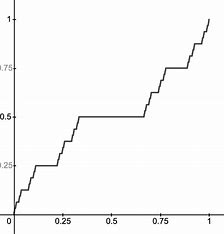
\includegraphics[width=0.5\linewidth]{REU-2024//Images/Cantor function.png}
    \caption{Cantor function}
\end{figure}

\prop{Suppose $A\subset [0,1]$ is a Lebesgue measurable set. Let $m$ be Lebesgue measure:
\begin{enumerate}
    \item For all $\epsilon>0,$ there exists an open set $G$ such that $m(G - A) < \epsilon$ and $A\subset G.$
    \item For all $\epsilon>0,$ there exists a closed set $F$ such that $m(A-F)< \epsilon$ and $F\subset A.$
    \item There exists a set $H$ which contains $A$ that is the countable intersection of a decreasing sequence of open sets and $m(H-A) = 0.$
    \item There exists a set $F$ which is contained in $A$ that is the countable union of an increasing sequence of closed sets which is contained in $A$ and $m(A - F) = 0.$
    \cor{Let $\mu$ be a Lebesgue-Stietljes measure on the real line. The conclusion of the above proposition holds with $m$ replaced by $\mu.$}
\end{enumerate}}

\section{Nonmeasurable Sets}
\thm{Nonmeasurable sets}{Let \[m^* = \inf\{\sum_{i = 1}^\infty \ell(A_i) | A_i \in \calC \quad \text{and} \quad E \subset \bigcup_{i=1}^\infty A_i\}\], where $\calC$ is the collection of intervals that are open on the left and closed on the right and $\ell((a,b]) = b-a.$ $M^*$ is not a measure on the collection of all subsets of $\bbR.$}
\pf{Suppose $m^*$ is a measure, and define $x\sim y$ if $x-y$ is rational. For each equivalence class, pick an element out of that class and call the collection of these points $A.$ Given a set $B,$ define $B+x = \{y + x | y \in B\}.$ Note that $\ell((a + q, b+q]) = b-a = \ell((a,b])$ for all $a,b q,$ and thus $m^*(A + q) = m^*(A)$ for each $A$ and $q.$ Moreover, $A+q$ are disjoint for different rationals $q.$ Now, consider that \[[0,1]\subset \bigcup_{q\in [-1,1]\cap \bbQ}(A+q),\] and thus $1\leq \sum_{q\in [-1,1]\cap \bbQ}m^*(A+q),$ and thus $m*(A)>0.$ Consider now that \[ \bigcup_{q\in [-1,1]\cap \bbQ}(A+q)\subset [-1,2],\] and thus $3\geq \sum_{q\in [-1,1]\cap \bbQ}m^*(A+q),$ implying that $m*(A) = 0,$ a contradiction.}

\section{The Caratheodory Extension Theorem}
Let $\calA_0$ be an algebra. Saying that $\ell$ is a measure means that: $\ell(\emptyset) = 0$ and if $A_i \in \calA_0$ pairwise disjoint and their union is in $\calA_0,$ then (2) of the definition of a measure holds. A measure on an algebra is often referred to as a \textit{premeasure}. 
\thm{The Caratheodory Extension Theorem}{Suppose $\calA_0$ is an algebra and $\ell: \calA_0 \to [0,\infty]$ is a measure on $\calA_0.$ Define \[\mu^*(E) = \inf\{\sum_{i = 1}^\infty \ell(A_i) | \text{each} A_i \in \calA_0, E \subset \bigcup_{i=1}^\infty A_i\}\] for $E\subset X.$ Then:
\begin{enumerate}
    \item $\mu*$ is an outer measure;
    \item $\mu*(A) = \ell(A)$ if $A \in \cal(A_0);$
    \item Every set in $\calA_0$ and every $\mu^*-$null set is $\mu^*-$measurable;
    \item If $\ell$ is $\sigma-$finite, then there is a unique extension to $\sigma(\calA_0).$
\end{enumerate}}

\chapter{Measurable functions}

\section{Measurability}
Suppose we have a measurable space $(X,\calA).$
\defn{Measurable function}{A function $f: X\to \bbR$ is \textit{measurable} or $\calA $ measurable if $\{x | f(x) >a\}\in \calA$ for all $a\in \bbR.$ A complex-valued function is measurable if both the real and imaginary are measurable.}
\rmk{The preimage of $(a, \infty]$ is measurable under $f.$}

\rmkb{In other words, if $(\Omega_1, \calA_1)$ and $(\Omega_2, \calA_2)$ are measurable sets, $f: \Omega_1 \to \Omega_2$ is measurable if $f^{-1}(A_2) \in \calA_1$ for all $A_2 \in \calA_2.$}

\ex{
Suppose $f$ is a real valued function and identically constant, then the set $\{x | f(x)> \alpha\}$ is either empty or all of $X,$ so $f$ is measurable.
}

\ex{Define
\[f(x) := \begin{cases}
    1, \qquad x \in A\\
    0 \qquad x\notin A
\end{cases},\] then $\{x | f(x)>a\}$ is either $\emptyset, A, X,$ and thus $f$ is measurable if and only if $A \in \calA.$}

\ex{Suppose $X\in \bbR$ with $\calB$ measure, then $f(x) = x$ yields $\{x |f(x)>a\} = (a,\infty)$ is measurable. }

\prop{Suppose $f$ is real valued. The following are equivalents:
\begin{enumerate}
    \item $\{x | f(x)>a\}$ for all $a\in \bbR.$
    \item $\{x | f(x)<a\}$ for all $a\in \bbR.$
    \item $\{x | f(x)\leq a\}$ for all $a\in \bbR.$
    \item $\{x | f(x) \geq a\}$ for all $a\in \bbR.$
\end{enumerate}
}
\pf{
\[\{x | f(x)\leq a\} = \{x | f(x)>a\}^c\] and thus if the latter is $\calA$ measurable, then the former will be. Moreover, note that \[\{x | f(x)\geq a\} = \bigcap_{i= 1}^\infty\{x | f(x)> a - \frac{1}{n}\}\]
}

\prop{If $X$ is a metric space, $f$ is continuous, and $\calA$ contains all the open sets, then $f$ is measurable}
\pf{$\{x | f(x)>a\} = (a,\infty)$ is open, and thus in $\calA.$}

\prop{Let $c\in \bbR.$ If $f,g$ are measurable, then:
\begin{enumerate}
    \item $f + g;$
    \item $f - g;$
    \item $cf;$
    \item $fg;$
    \item $f \wedge g;$
    \item $f \vee g,$
\end{enumerate} are all measurable}

\pf{:\\
\begin{enumerate}
    \item Consider that if $f(x)  + g(x)< a,$ then there exists an $r\in \bbQ$ such that $f(x)<r< a + r,$ and thus:
    \[\{x | f(x) + g(x) < r\} \qquad \bigcup_{r\in \bbQ}(\{x | f(x) < r\} \cap \{x | g(x)< a + r\}\] and thus $f + g$ is measurable.
    \item Bootleg using Prop 5.1.3.
    \item If $c>0,$ then $\{x | cf(x) < a\} = \{x | f(x) < \frac{a}{c}\},$ and thus $cf$ is measurable. If $c = 0,$ use Example 1. If $c<0,$ bootleg as before.
    \item Notice first that
    \[\{x  | fg>a\} = \{x | \frac{1}{2}[(f + g)^2 - f^2 - g^2\}\] and thus it suffices to show that $f^2$ is measurable if $f$ is measurable. Consider that $\{x | f^2(x)>a\} = \{x | f(x)>\sqrt{a}\}\cup \{x | f(x)< -\sqrt{a}\}.$
    \item Obvious
\end{enumerate}
}

\prop{
If $f_i$ is a measurable function for each $i,$ then:
\begin{enumerate}
    \item $\sup(f_i)$
    \item $\inf(f_i)$
    \item $\lim_{i\to \infty}\sup(f_i)$
    \item $\lim_{i\to \infty}\inf(f_i)$
\end{enumerate}
}
\pf{
$\{x | \sup(f_i(x))>a\}  = \bigcup_{i = 1}^\infty\{x | f_i(x)>a\},$ and is therefore measurable.
}

\defn{Almost Everywhere}{We say $f=g$ \textit{almost everywhere} written $f = g$ a.e. if $\{x | f(x)\neq g(x)\}$ has measure zero.\newline Similarly, we write that $f_i \to f$ a.e if the set of $x$ where $f_i(x)$ does not converge to $f(x)$ has measure zero.}

\rmkb{If $X$ is a metric space and $\calB$ is the Borel $\sigma-$algebra and $f: X \to \bbR$ is measurable with respect to $\calB,$ we say $f$ is Borel measurable. Similarly, we would say something similar with respect to lebesgue measure.}

\prop{If $f: \bbR \to \bbR$ is monotone, then $f$ is Borel measurable.}
\pf{Suppose $f$ is increasing. Let $a\in \bbR$ and define $x_0 = \sup\{y | f(y)\leq a\}.$ If $f(x_0)\leq a,$ then $\{x | f(x)>a\} = (a,\infty).$ If $f(x_0)>a,$ then $\{x | f(x)>a\} = [x,\infty).$ Either case is Borel measurable.}

The following proposition states that if $f$ is measurable, then the inverse of a borel set is measurable:
\prop{Let $(X,\calA)$ be a measurable space and let $f: X \to \bbR$ be an $\calA$ measurable function. If $A\in \calB$ on $\bbR,$ then $f^{-1}(A)\in \calA.$ }
\pf{
Let $\calB$ be a Borel $\sigma-$algebra and $\calC = \{A \subset \bbR | f^{-1}(A)\in \calA\}.$ Note that \[f^{-1}\bigcup_{i=1}^\infty A =\bigcup_{i=1}^\infty f^{-1}(A)\in \calA,\] and thus $\calC$ is closed under unions (and by a similar proof, complements). Thus, $\calC$ is a $\sigma-$algebra. Since $f$ is measurable, $\calC$ contains $(a,\infty)$ for all $a.$ Therefore, $\calC$ contains $\calB.$ 
}

\ex{Constructing a set that is Lebesgue measurable but not Borel measurable:
\newline\newline
Let $f$ be the Cantor-Lebesgue function, and define \[F(x) = \inf\{y| f(y)\geq x\}\] Note that $F$ is increasing (but not continuous), and is defined to go from $[0,1]$ to $C,$ the Cantor set. By Proposition 5.1.7, $F^{-1}$ maps Borel sets back to Borel sets. Let $m$ be the Lebesgue measure and $A$ be the nonmeasurable set constructed at the end of the previous chapter. Let $B = F(A).$ Consider that because $F(A)\subset C,$ and $m(C) = 0,$ then $B$ is a null set, and thus $m$ measurable. However, $B$ is not Borel measurable, for if it where, then by the previous reasoning, $F^{-1}(F(A)) = A$ would be Borel measurable.
}

\section{Approximating Functions}

\defn{Characteristic Functions}{Let $(X, \calA)$ be a measurable space. If $E\in \calA,$ then the \textit{characteristic function} of $E$ is defined by \[\chi_E(x) = \begin{cases}
    1, x \in E\\
    0, x\notin E
\end{cases}\]}
\defn{Simple Function}{A \textit{simple function}, $s,$ is a function of the form
\[s(x) = \sum_{i=1}^na_i\chi_{E_i}(x)\] for real numbers $a_i$ and measurable sets $E_i.$}

\prop{Suppose $f$ is a non-negative and measurable function. Then there exists a sequence of non-negative measurable simple functions, $s_n,$ increasing to $f.$}
\pf{Let $A_{in} = \{x | \frac{i-1}{2^n}\leq f(x) < \frac{i}{2^n}\}$ and 
\[B_n  = \{x | f(x)\geq n\}\]. Then define \[s_n = \sum_{i=1}^{n2^n}\frac{i-1}{2^n}\chi_{A_{in}}+ n\chi_{B_n}\]
}

\section{Lusin's Theorem}
Recall that the \textit{support} of a function $f$ is the closure of the set $\{x | f(x)\neq 0\}$
\thm{Lusin's Theorem}{Suppose $f: [0,1]\to \bbR$ is Lebesgue measurable, $m$ is Lebesgue measure, and $\epsilon>0.$ There exists a closed set $F\subset [0,1]$ such that $m([0,1] - F)< \epsilon$ and the restriction of $f$ to $F$ is a continuous function on $F.$}
\rmk{Loosely, this means that every measurable function is almost continuous}

\chapter{The Lebesgue Integral}

\defn{The Lebesgue Integral}{Let $(X,\calA, \mu)$ be a measure space. If \[s = \sum_{i=1}^na_i\chi_{E_i}\] is a non-negative measurable simple function, then define the \textit{Lebesgue integral} of $s$ to be:
\[\int s d\mu = \sum_{i=1}^n a_i \mu(E_i).\] If $a_i = 0$ and $\mu(E_i) = \infty$, we the convention that $a_i\mu(E_i) = 0.$ If $f\geq 0$ is a measurable function, then define
\[\int f d\mu = \sup \left\{\int s d\mu: 0 \leq s \leq f, s \textit{simple}\right\}\]\newline\newline
Let $f$ me measurable and $f^{+} = \max(f,0)$ and $f^{-}= \max (-f,0).$ Provided neither of those are finite, define
\[\int f d\mu  = \int f^+ d\mu  - \int f^- d\mu\] Finally, if $f = u + iv$ is a complex value function and $\int(|u| + |v|)d\mu$ is finite, then define
\[\int f d\mu = \int ud\mu  + i \int v d\mu\]}

\defn{Integrable}{If $f$ is measurable and $\int |f| d \mu < \infty,$ then $f$ is \textit{integrable}.}

\prop{
\begin{enumerate}
    \item If $f$ is a real value measurable function with $0\leq a \leq f(x) \leq b$ for all $x$ and $\mu(X)< \infty,$ then $a\mu(X) \leq \int fd\mu \leq b\mu(X).$
    \item If $f$ and $g$ are measurable, real valued, and integrable and $0\leq f(x) \leq g(x)$ for all $x,$ then $\int f d\mu \leq g d\mu.$
    \item If $f$ is a real valued non-negative, and integrable and $c$ is a non-negative real number, then $\int c f d\mu = c\int f d\mu.$
    \item If $\mu(A)=0$ and $f$ is non-negative and measurable, then $\int f\chi_Ad\mu = 0.$
\end{enumerate}
}






\chapter{Probability}

\defn{Probability Space}{A \textit{probability space} is a triple $(\Omega, \calF, \bbP),$ where $\Omega$ is an arbitrary set, $\calF$ is a $\sigma-$field of subsets of $\Omega,$ and $\bbP$ is a probability on $(\Omega,\bbP)$.}
\defn{Probability}{A \textit{probability}, or \textit{probability measure}, is a positive measure whose total mass is 1, so that $\bbP(\Omega) = 1.$ }
\rmkb{Elements of $\bbF$ are called events, elements of $\Omega$ are denoted by $\omega.$}

\defn{Almost Surely}{Instead of saying a property occurs almost everywhere, we talk about properties occurring \textit{almost surely}, or \textit{a.s.}}

\defn{Random Variables}{Real-valued measurable functions from $\Omega$ to $\bbR$ are \textit{random variable} and usually denoted by $X$ or $Y$ and abbreviated by $r.v.$}

\defn{Expectation}{The Lebesgue integral of a random variable $X$ with respect to a probability measure $\bbP$ is called the \textit{expectation} or the \textit{expected value} of $X,$ and we write $\bbE[X]$ for $\int X d\bbP.$ The notation $\bbE[X; A]$ is used for $\int_A X d\bbP.$}

\defn{Indicator}{The random variable $1_A$ is the function defined by
\[1_A = \begin{cases}
    1, \qquad \omega \in \Omega
    0, \qquad \omega\notin \Omega
\end{cases}\] is defined to be the \textit{indicator} of $A.$}

\rmkb{Events such as $\{\omega | X(\omega) >a\}$ are almost always abbreviated by $(X>a).$ Thus, \[X>a, Y>b\] refers to $\{w| X(\omega)>a \quad \text{and}\quad Y(\omega) >b\}$}

\defn{$\sigma-$fields genererated by $X.$}{Given a random variable $X,$ the $\sigma-$field generated by $X,$ denoted by $\sigma(X),$ is the collection of events $(X\in A),$ $A$ being a Borel subset of $\bbR.$ If we have several random variables: $X_1, $X_2, \dots, X_n, we write $\sigma(X_1, \dots, X_n)$ for the $\sigma$ field generated by the collection of events 
$\{X_i \in A | A \in \calB\}$}


\rmkb{Remember from before that the notation $X\in A$ is used to signify $\{\omega | X(\omega)\in A\}.$}

\defn{Distribution}{Given a random variable $X,$ we can define a probability on $(\bbR, \calB),$ by 
\[\bbP_X(A) = \bbP(X\in A), \qquad A \in \calB.\] This probability $\bbP_X$ is known as the \textit{law} or \textit{distribution} of $X.$}

\defn{Distribution function}{Define a function $F_X: \bbR \to [0,1]$ by \[F_X(x) = \bbP_X((-\infty, x]) = \bbP(X\leq x).\] Such a function $F_x$ is called the \textit{distribution function} of $X.$ Note that $F_X$ is an increasing function whos corresponding Lebesgue-stietjes measure is $\bbP_x.$}

\prop{The distribution function $F_X$ of a random variable satisfies:
\begin{enumerate}
    \item $F_X$ is increasing.
    \item $F_X$ is right continuous.
    \item \[\displaystyle\lim_{x\to \infty}F_X(x) =1 \qquad \displaystyle\lim_{x\to -\infty}F_X(x) =0\]
\end{enumerate}
}

\prop{Suppose $F$ is a distribution function. There exists a random variable $X$ such that $F = F_X.$}

\pf{Let $\Omega = [0,1]$ $\calF$ be the Borel $\sigma-$field, and $\bbP$ the Lebesgue measure. Define $X(\omega) = \sup(y | f(y)< \omega)$ If $X(\omega)\leq x,$ then $F(y)>\omega$ for all $y>x.$ By right continuity, $F(x)\geq \omega.$ On the other hand, if $\omega \leq F(x),$ then $x\notin \{y: F(y)< \omega\},$ and thus $X(\omega)\leq x$. Thus, $\{\omega | X(\omega)\leq x\} = \{\omega | 0\leq e\omega \leq F(x)\},$ and thus $F_x(x) = F(x).$}

The following are examples of various distributions:
\ex{Bernoulli: A random variable $X$ is a Bernoulli random variable with parameter $p$ is $\bbP(X = 1) = p$ and $\bbP(X = 0) = 1 -0$ for some $p\in [0,1].$}
\ex{Binomial: A random variable $X$ is a binomial random variable with parameters $n$ and $p$ if $P(X = k) = \binom{n}{k}p^k(1-p)^{n-k},$ where $n\in \bbN$ and $0\leq k \leq n$ and $ p \in [0,1].$}
\ex{A random variable $X$ is a geometry random variable with parameter $p$ if $\bbP(X = k) = (1-p)p^k,$ where $p \in \bbZ_+$}
\ex{Poisson: If $\bbP(X = k) = \frac{e^{-\lambda}\lambda^k}{k!}$ for $k\in \bbZ_+$ and $\lambda>0,$ then $X$ is a Poisson random variable with parameter $\lambda.$}
\defn{Density}{If $F$ is absolutely continuous, we call $f = F'$ the \textit{density} of $F.$}
\ex{Exponential: Let $\lambda>0.$ For $x>0,$ let $f(x) = \lambda^{-\lambda x}.$ If $X$ has a distribution function who's density is equal to $f,$ then $X$ is an exponential random variable with parameter $\lambda.$}
\ex{Standard Normal: Define $f(x) = \frac{1}{\sqrt{2\pi}}e^{\frac{-x^2}{2}}.$ If the distribution function of $X$ has $f$ as its density, then $X$ is a standard normal variable, and so:
\[\bbP(X\in A) = \bbP_X(A) = \frac{1}{\sqrt{2\pi}}\int_Ae^{\frac{-x^2}{2}}\]}

\prop{Suppose $g$ is Borel measurable and $g$ is either bounded or non-negative. Then
\[\bbE [g(X)] = \int g(x)\bbP_X(dx)\]}
\pf{If $g$ is the indicator function of an event $A,$ this becomes the definition of $\bbP_X.$ By linearity, the results holds for simple functions $g.$ By approximating a non-negative measurable function from below by simple functions, the result holds for non-negative functions $g$ and thus by linearlity, for bounded and measurable $g.$}

\rmkb{If $F_X$ has density $f_x,$ then $\bbP_X(dx) = f_x(x)dx.$ If $X$ is integrable ($\bbE[X]< \infty,$) we have that \[\bbE[X] = \int xf_X(x)dx\qquad \bbE[X^2] = \int x^2 f_X(x)dx\]}
\newcommand{\Var}{\text{Var}}
\defn{Mean}{We define the \textit{mean} of a random variable to be its expectation}
\defn{Variance}{We define the \textit{variance} of a random variable to be
\[\Var(X) = \bbE(X - \bbE(X))^2\]}
\rmkb{$\Var(X+c) = \Var(X)$}
\rmkb{\[\Var(X) = \bbE(X - \bbE X)^2 = \bbE[X^2 - 2X\bbE X + (\bbE X)^2 = \bbE X^2 - (\bbE X)^2.]\] Therefore, $\Var(X)\leq \bbE X^2$ and $\Var(cX) = c^2\Var(X)$ for any constant $c.$}
\prop{If $X\geq 0$ a.s. and $p>0,$ then
\[\bbE[X^p] = \int_0^\infty p\lambda^{p-1}\bbP(X>\lambda)d\lambda\]
}
\pf{Using Fubini's Theorem:
\[\int_0^\infty p\lambda^{p-1} \bbP(X>\lambda)d\lambda = \bbE\int_0^\infty p\lambda^{p-1}1_{(\lambda, \infty)}(X)d\lambda= \bbE\int_0^\infty p\lambda^{p-1}d\lambda = \bbE X^p\]}

\prop{Suppose $g$ is convex and $X$ and $g(X)$ are both integrable. Then $g(\bbE X)\leq \bbE(g(X)).$}

\section{Independence}
\defn{Independent}{Two events $A$ and $B$ are independent if $\bbP(A\cap B) = \bbP(A)\bbP(B).$ The events $A_1, \dots, A_n$ are linearly independent if 
\[\bbP(A_{i_{1}}\cap A_{i_{2}}\cap \cdots \cap A_{i_j}) = \bbP(A_{i_1})\bbP(A_{i_2})\cdots \bbP(A_{i_j})\] whenever $1\leq i_1 < \dots < i_j \leq n.$}
\ex{Given $n =3,$ we have that $\bbP(A_1 \cap A_2 \cap A_3)$ must factor properly, but $\bbP(A_1 \cap A_2), \bbP(A_1 \cap A_3),$ and $\bbP(A_2 \cap A_3)$ must do the same.} 

\prop{If $A$ and $B$ are independent, then $A^C$ and $B$ are independent}
\pf{\[\bbP(A^C \cap B) = \bbP(B) - \bbP(A\cap B) = \bbP(B) - \bbP(A)\bbP(B) = \bbP(1 - \bbP(A)) = \bbP(B)\bbP(A^C)\]}

\rmkb{We say $\calF$ and $\calG$ are independent $\sigma-$fields if $A$ and $B$ are independent whenever $A\in \bbF$ and $B \in \bbG.$ \newline\newline We say $X$ and $Y$ are two independent random variables if $\sigma(X)$ and $\sigma(Y)$ are independent.}

\rmkb{Given an infinite sequence of events $\{A_n\},$ we say that they are independent if any finite subset of them is independent.}

\rmkb{If $f$ and $g$ are Borel functions and $X$ and $Y$ are independent, then $f(X)$ and $g(Y)$ are independent. This is because $\sigma(f(x))\subset \sigma(X)$ and same for $\sigma(g(y)) \subset \sigma(Y).$}


\defn{Infinitely Often}{If $\{A_n\}$ is a sequence of events, define $A_n$ i.o ($A_n$ \textit{infinitely often}), by 
\[(A_n \text{i.o.}) = \bigcap_{n=1}^\infty \bigcup_{i=n}^\infty A_i\]}

\lem{Borel-Cantelli Lemma}{Let$\{A_n\}$ be a sequence of events.
\begin{enumerate}
    \item If $\sum_{n}\bbP(A_n)< \infty,$ then $\bbP(A_n \text{i.o.})<  = 0.$
    \item If $A_n$ are independent events and $\sum_n\bbP(A_n) = \infty,$ then $\bbP(A_n \text{i.o.}) = 1.$
\end{enumerate}
}
\pf{:\\
\begin{enumerate}
    \item \[\bbP(A_n \text{i.o.}) = \lim_{n\to \infty} \bbP(\bigcup_{i=n}&\inftyA_i) \leq \sum_{i = n}^\infty \bbP(A_i)\] which the RHS tends to zero as $n\to \infty.$
    \item \[\bbP(\bigcup_{i=n}&\inftyA_i) = 1- \bbP(\bigcap_{i=n}&\inftyA_i^C) = 1- \prod_{i=n}^N \bbP(A_i^C) = 1- \prod(1-\bbP(A_i))\] and thus because $1 - e^{-x}\leq x,$ we have that the RHS is greater than or equal to \[1 - e^{-\sum_{i=n}^N \bbP(A_i)},\] which tends to $1$ as $N \to \infty.$
\end{enumerate}
}

\thm{Multiplication Theorem}{If $X,y$ and $XY$ are integrable and $X$ and $Y$ are independent, then $\bbE[XY] = \bbE[X]\bbE[Y].$}

\rmkb{If $X_1, \dots, X_n$ are independent, then so are the random variable $X_1 - \bbEX_1, \dots, X_n - \bbE X_n.$ Moreover, using the multiplication theorem to show that cross product terms are zero, we have that \[\bbE[(X_1 - \bbEX_1) + \dots + (X_n - \bbE X_n)]^2 = \bbE(X_1 - \bbEX_1)^2 + \dots + \bbE(X_n - \bbEX_n)^2\] Therefore, if the $X_i$ are independent, then the variance of the sum is equal to the sum of the variances.}

\section{Weak Law of Large Numbers}
\defn{Independent and Identically Distributed}{Given that $X_n$ is a sequence of independent random variables, we have that $\bbP_{X_n} = \bbP_{X_1}$ (all r.v. have the same distribution). This situation is \textit{i.i.d}}

\rmkb{In i.i.d, we have that $\bbP(X_n \in A) = \bbP(X_1 \in A)$ and for all $n$ and Borel sets $A.$ Moreover, we have that $\bbE X_n = \bbE X_1$ and $\Var X_n = \Var X_1.$}

\defn{Partial Sum Process}{Define a \textit{partial sum process} to be \[S_n = \sum_{i=1}^n X_i\]. }
\rmkb{This means that $\frac{S_n}{n}$ is the average value of the first $n$ of the $X_i'$s.}

\defn{Converges in probability}{We say that a sequence of random variables $\{Y_n\}$ \textit{converges in probability} to a random variable $Y$ if it converges in measure with respect to the measure $\bbP.$ This emans that for all $\epsilon>0,$ we have that, as $n\to \infty,$ \[\bbP(|Y_n - Y|>\epsilon)\to 0\]}

\thm{Weak Law of Large Numbers}{Suppose the $X_i$ are i.i.d. and $\bbE[X_1^2]<\infty.$ Then $\frac{S_n}{n}\to \bbE[X_1]$ in probability.}
\pf{Since $X_i$ are i.i.d, then for $n$ large enough, we have that $\bbE S_n = n \bbE X_1.$ Therefore, $\bbE[(\frac{S_n}{n} - \bbE X_1)^2]$ is the variance of $\frac{S_n}{n}.$ Let $\epsilon>0.$ We know by \textit{Chebyshev's inequality} that \[\bbP(|\frac{S_n}{n} - \bbE[X_1]|>\epsilon|) = \bbP((\frac{S_n}{n} - \bbE[X_1])^2>\epsilon^2)\leq \frac{\Var(\frac{S_n}{n})}{\epsilon^2} = \frac{\sum_{i=1}^n\Var X_i}{n^2\epsilon^2}= \frac{n\Var X_1}{n^2\epsilon^2}\] which the RHS converges to $0$ as we let $n\to \infty.$}

\ex{If $S_n$ is the sum of i.i.d. Bernoulli random variables $X_1, \dots, X_n,$ then $S_n$ is the number of the $X_i$ that are equal to $1.$ The probability that the first $k$ are $X_i's$ and the rest are $0$ is $p^k(1-p)^{n-k},$ and we get the same probability for any configuration of $k$ ones. Therefore, $\bbP(S_n = k) = \binom{n}{k}p^k(1-p)^{n-k}.$}

\section{Strong Law of Large Numbers}
\thm{Strong Law of Large Numbers}{Suppose $\{X_i\}$ is an i.i.d. sequence with $\bbE[|X_1|]<\infty.$ Let $S_n = \displaystyle\sum_{i=1}^nX_i.$ Then
\[\frac{S_n}{n}\to \bbE{X_1},\qquad \text{a.s.}\]}

The following Lemmas are useful in proving the SLoFG

\lem{}{If $X\geq 0$ a.s. and $\bbE[X]< \infty,$ then \[\sum_{n=1}^\infty \bbP(X\geq n) < \infty\]}
\pf{
Since $\bbP(X\geq x)$ increases as $x$ decreases, then 
\[\sum_{n=1}^\infty \bbP(X\geq n)\leq \sum_{n=1}^\infty \int_{n-1}^n \bbP(X\geq x)dx = \int_0^\infty \bbP(X\geq x)dx = \bbE[X]\]
}

\section{Conditional Expectation}
Informally, one can think that if $X$ is a random variable, then $\bbE[X]$ is the best guess for $X$ given no information about the result of the trial. A conditional expectation can be thought of as the best guess given a little bit of information.\newline\newline

It is common in probability theory for there to be more than one $\sigma-$field present. For example, if $X_1, X_2\dots$ is a sequence of random variables, then one can define $\calF_n = \sigma(X_1, \dots, X_n),$ and thus $\calF$ is generated by the collection of sets $(X_i \in A)$ and $A\in \calB.$ Thus, we can think of $\bbF_n$ as the information that is contained in $X_1, X_2, \dots, X_n.$ Thus, it makes sense to write $\bbE[Y | X_1, \dots, X_n]$ and $\bbE[Y | \calF_n]$ and that $\calF_0$ stands for no information. 

\defn{Conditional Expectation}{If $\calF \subset \calG$ are two $\sigma-$fields and $X$ is an integrable $\calG$ measurable random variable, then the \textit{conditional expectation} of $X$ given $\calF,$ written $\bbE[X  | \calF],$ is any $\calF$ measurable random variable $Y$ such that $\bbE[Y | A] = \bbE[X | A]$ for all $A\in \calF$}
\defn{Conditional Probability}{The \textit{conditional probability} of $A\in \calG$ given $\bbF$ is defined by $\bbP(A | \calF) = \bbE[1_A | \calF].$ When $\calF = \sigma(Y),$ one usually writes $\bbE[X | Y]$ for $\bbE[C | \calF].$}
There are a couple properties this contains:
\begin{enumerate}
    \item The best guess should just be the expected value if there is no new information, and thus $\bbE[X | \calF_0]  = \bbE[X].$
\end{enumerate}

\rmkb{If $Y_1,Y_2$ are two $\calF$ measurable random variables such that $\bbE[Y_1 | A] = \bbE[Y_2 | A]$ for all $A\in \calF,$ then $Y_1 = Y_2$ a.s.}

\rmkb{If $X$ is already $\calF$ measurable, then $\bbE[X | \calF] = X.$}

\ex{Suppose that $X,Y$ have a joint density $f(x,y), \qquad 0< x,y< \infty$ with marginal densities \[f(x) = \int_{-\infty}^\infty f(x,y)dy, \qquad g(y) = \int_{-\infty}^\infty f(x,y)dx\] Thus, the conditional density $f(y| x)$ is defined by
\[f(y|x) = \frac{f(x,y)}{f(x)}\] and thus 
\[\bbE[Y | X=x] = \int_{-\infty}^\infty yf(y | x)dy\]. An interesting fact arises:
\begin{align*}
    \bbE[\bbE[Y | X]] &= \int_{-\infty}^\infty[Y = X = x]f(x)dx\\
    &= \int_{-\infty}^\infty [\int_{-\infty}^\infty yf(y | x)dy] f(x)fx\\
    &= \bbE[Y]
\end{align*}}
\newpage

\prop{If $X$ is independent of $\calF,$ $\bbE[X | \calF] = \bbE[X].$}
\pf{If $A\in \calF,$ then $1_A$ and $X$ are independent, and by the multiplication theorem:
\[\bbE[X | A] = \bbE[X1_A] = \bbE[X]\bbE[1_A] = \bbE[\bbE[X | A]].\]}

\ex{Suppose $\{A_i\}$ is a collection of finite disjoint sets who's union is $\Omega,$ $\bbP(A_i)>0$ for all $i,$ and $\bbF$ is the $\sigma-$field generated by the $A_i's.$ Then:
\[\bbP(A  | \calF) = \sum_{i}\frac{\bbP(A\cap A_i)}{\bbP(A_i)1_{A_i}}\] This follows because 
\[\bbE[\sum_i \frac{\bbP(A\cap A_i)}{\bbP(A_i)}1_[A_i] | A_j] = \frac{\bbP(A\cap A_j)}{\bbP(A_j)}\bbE[1_{A_j} | A_j] = \bbP(A \cap A_j).\]
}

\ex{For a concrete example, suppose we toss a fair coin independently $5$ times and let $X_i$ be $1$ or $0$ depending whether the $i^{th}$ toss was a heads or tails. Let $A$ be the event that there were $5$ heads and let $\calF_i = \sigma(X_1, \dots, X_i).$ Therefore, $\bbP(A) = \frac{1}{32}$ while \[\bbP(A | \calF_1) = \begin{cases}
    \frac{1}{16}, \qquad X_1 = 1\\
    0, \qquad X_1 = 0
\end{cases}\] }

\prop{If $\calF \subset \calG$ and $X$ is integrable and $\calG$ measurable, then 
\[\bbE[\bbE[X | \calF]] = \bbE[X]\]}
\pf{\[\bbE[\bbE[X | \calF]] = \bbE[\bbE[X | \calF] | \Omega] = \bbE[X | \Omega] = \bbE[X]\]}
\rmkb{From this we can derive a property that is sometimes used in the definition of conditional probability:
For every $\calF_n-$measurable event $A,$ we have that 
\[\bbE[\bbE[Y | \calF_n]1_A] = \bbE[Y1_A]\]}


\prop{:\\
\begin{enumerate}
    \item If $X\geq Y$ are both integrable, then 
    \[\bbE[X | \calF]\geq \bbE[Y | \calF], \qquad a.s.\]
    \item If $X$ and $Y$ are integrable and $a\in \bbR,$ then 
    \[\bbE[aX + y | \calF] = a\bbE[X | \calF] + \bbE[Y | \calF]\]
\end{enumerate}
}

\prop{(Jensen's Inequality for conditional expectations). If $g$ is convex and $X$ and $g(X)$ are integrable, then 
\[\bbE[g(X) | \calF]\geq g(\bbE[X  | \calF]), \qquad a.s.\]}

\prop{If $X$ and $XY$ are integrable and $Y$ is $\calF$ measurable, then \[\bbE[XY | \calF] = Y \bbE[X | \calF].\]}
\pf{
If $A \in \calF,$ then for any $B \in \cal F,$
\[\bbE[1_A \bbE[X | \calF]; B] = \bbE[\bbE[X | \calF]; A\cap B] = \bbE[X; A\cap B] = \bbE[1_AX; B].\]
Using the same technique of linearity and approximating the simple random variable to $Y$ shows that the theorem is done.
}

\prop{If $\mathcal{E} \subset \calF \subset \calG.$ then \[\bbE[\bbE[X | \calF] | \mathcal{E}] = \bbE[X | \mathcal{E}] = \bbE[\bbE[X | \mathcal{E}] | \calF]\]}
\pf{The second equality holds because $\bbE[X | \mathcal{E}]$ is $\mathcal{E}$ and thus $\calF$ measurable. For the first equality, let $A \in \mathcal{E}.$ Thus, since $A\in \calF,$ 
\[\bbE[\bbE[\bbE[X | \calF] | \mathcal{E}]; A]= \bbE[\bbE[X | \calF]; A] = \bbE[X;A] = \bbE[\bbE[X | \mathcal{E}]; A].\]
}

\prop{If $X$ is integrable, then $\bbE[X | \calF]$ exists.}

\pf{Using Radon-Nikodym Theorem}

\prop{(Tower Property): If $m< n,$ then 
\[\bbE[\bbE[Y | \calF_n] | \calF_m] = \bbE[Y | \calF_m].\]}

\ex{Suppose $X_1, \dots, X_n$ are independent random variables with $\bbE[X_j] = \mu,$ for each $j.$ Let $S_n = \sum_{{j=0}}^n X_j$ and let $\bbF_n$ be the information contained in $X_1, \dots, X_n$ ($\sigma(X_1, \dots, X_n).$), then if $m< n,$ we have that 
\begin{align*}
    \bbE[S_n | \calF_m] &= \bbE[S_m | \calF_m] + \bbE[S_n - S_m | \calF_m]\\
    &= S_m + \bbE[S_n - S_m]\\
    &= S_m + \mu(n-m)
\end{align*}
}

\ex{Same example as before, but now suppose $\mu = 0$ and $\bbE[X_j^2] =\sigma^2$:
\begin{align*}
    E[S_n^2 | \calF_m] &= \bbE[(S_m + (S_n - S_m))^2 | \calF_m]\\
    &= \bbE[S_m^2 | \calF_m] + 2\bbE[S_m(S_n -  S_m) | \calF_m] + \bbE[(S_n - S_m)^2 | \calF_m]\\
    &= S_m^2 + \sigma^2(n-m)\\
\end{align*}
}


\section{Martingales}
\defn{Filtration}{If $X_1, X_2, \dots, X_n$ is a sequence of random variables, then the associated (discrete time) \textit{filtration} is the collection $\{\calF_n\}$ where $\calF_n$ denotes the information in $X_1, \dots, X_n,$ i.e, the $\sigma-$algebra generated by said random variables.}

\defn{Adapted}{Let $\calF$ be a $\sigma-$field and let $\{\calF_n\}$ be an increasing sequence of $\sigma-$fields each of which is contained in $\calF.$ That is, $\calF_1 \subset \calF_2 \subset \cdots$ and $\calF_n \subset \calF$ for each $n.$ A sequence of random variables $M_n$ is \textit{adapted} to $\{\calF_n\}$ if for each $n,$ $M_n$ is $\calF_n$ measurable.}

\defn{Martingale}{$M_n$ is a \textit{martingale} with respect to an increasing family of $\sigma-$fields $\{\calF_n\}$ if:
\begin{enumerate}
    \item $M_n$ is adapted to $\calF_n;$
    \item Each $M_n$ is integrable for each $n;$
    \item $\bbE[M_{n+1} | \calF_n] = M_n,\qquad a.s, \qquad n= 1,2,\dots$
\end{enumerate}
}
\rmkb{It is usually the case that $\calF_n = \sigma(M-1, \dots, M_n).$}
\rmkb{Note that it is easy to derive that for any martingale, we have that if $m<n,$ we have that \[\bbE[M_n | \calF_m]=  M_m\] and \[\bbE[M_n - M_m | \calF_m] = 0.\] Thus, we can say that if $M_n$ are the winnings of a game, no matter what happens up to time $m,$ the expected winnings in the next $n-m$ games is $0.$} 

\prop{If $M_n$ is a martingale, then \[\bbE[M_n] = \bbE[\bbE[M_n | \calF_0]] = \bbE[M_0].\] 


\pf{Proposition 7.4.4}}

\defn{Submartingale/Supermartingale}{If $X_n$ is a sequence of adapted integrable random variables with \[\bbE[X_{n+1} | \calF_n] \geq X_n,\qquad a.s, \qquad n= 1,2,\dots\], we call $X_n$ a \textit{submartingale}.\newline\newline If instead we have \[\bbE[X_{n+1} | \calF_n] \leq X_n,\qquad a.s, \qquad n= 1,2,\dots\], we call $X_n$ a \textit{supermartingale}.}

\ex{If $X_i$ is a sequence of mean zero integrable i.i.d. random variables and $S_n$ is the partial sum process, then $M_n = S_n$ is a martingale, since (using independence and the fact that $S_n$ is measurable with respect to $\calF_n$)
\[\bbE[M_{n+1} | \calF_n] = M_n + \bbE[M_{n+1} - M_n | \calF_n] = M_n + \bbE[M_{n+1} - M_n] = M_n + 0\] }
\ex{If the $X_i's$ have variance one and $M_n = S_n^2 - n,$ then, using independence,
\[\bbE[S_{n+1}^2 | \calF_n] = \bbE[(S_{n+1} - S_n)^2 | \calF_n] + 2s_n\bbE[S_{n+1} | \calF_n] - S_n^2 = 1+ S_n^2\]}

\ex{(Discrete Stochastic Integral) Suppose that $M_0, M_1, \dots$ is a martingale with respect to $\calF_n.$ For $n\geq 1,$ let $\Delta M_n = M_n -M_{n-1.}$ Let $B_j$ denote the "bet" of the $j$th game. We allot negative value of $B_j,$ which indicate betting that the price will go down or the game will be lost. Let $W_n$ denote the winnings of this strategy: $W_0 = 0$ and for $n\geq 1,$ we have that \[W_n = \sum_{j=1}^n B_j[M_j - M_{j-1} = \sum_{j=1}^n B_j \Delta M_j\] Let $B_n$ be $\calF_{n-1}$ measurable (we cannot see the result of the $n$th bet before betting.) The claim is that our winnings, $W_n$ are a martingale:
\begin{align*}
     \bbE[W_{n+1}  | \calF_n] &= \bbE[W_n + B_{n+1}(M_{n+1} - M_n) | \calF_n]\\
     &= \bbE[W_n | \calF_n] + \bbE[B_{n+1}(M_{n+1} - M_n) | \calF_n]\\
\tag{$W_n$ is $\calF_n$ measurable}     &= W_{n} + B_{n+1}\bbE[M_{n+1} - M_n | \calF_n]\\
&= W_n
\end{align*}
Therefore, one cannot change a discrete time martingale to a game in one's favor with a betting strategy in a finite amount of time. }

\ex{(Martingale Betting Strategy) Let $X_1, X_2, \dots$ be independent random variables with 
\[\bbP[X_j = 1] = \bbP[X_j = -1] = \frac{1}{2}\] Thus, let $M_0 = 0,$ $M_n = X_1 + X_2 + \dots  + X_n.$ Our betting strategy will be doubling our bet when we lose, and quitting when we win, thus assuring that once we win (which we will do almost surely), we will win $\$1.$ The winnings in the game can be written as 
\[W_n = \sum_{j=1}^n B_j \Delta M_j = \sum_{j=1}^n B_j X_j\] where $B_1 = 1$ and for $j>1:$
\[B_j = 2^{j-1} \qquad \text{if} X_1 = X_2 = \dots X_{j-1} = -1\] and $B_j = 0$ else.\newline\newline By the previous example, $W_n$ is a martingale. In particular, for each $n,$ $\bbE[W_n] = 0,$ which we can check that noting that $W_n = 1$ unless $X_1  = \dots = X_n = -1,$ in which case $W_n = -1 - 2 - 2^2 - \dots - 2^{n-1} = -[2^{n} -1],$ which happens with probability $(\frac{1}{2})^n.$ Thus, \[\bbE[1 \cdot [1 - \frac{1}{2^n}]] - [2^n -1]\cdot \frac{1}{2^n}\] However, we know that $\lim_{n\to \infty}W_n = 1,$ and thus $1 = \bbE[W_\infty]>\bbE[W_0] = 0,$ and thus we have a submartingale (or a game in our favor). }

\defn{Stopping Time}{Suppose we have an increasing sequence of $\sigma-$fields $\{\calF_n\}$ contained in a $\sigma-$field $\calF.$ Let $\calF_\infty = \sigma(\displaystyle\bigcup_{n=1}^\infty \calF_n).$ A random variable $N$ (which is $\calF$ measurable) from \[\Omega \to \{0,1,2,\dots\}\cup \{\infty\}\] is called a \textit{stopping time} if for each finite $n,$ we have that $(N\leq n)\in \calF_n.$}

\rmkb{Thus, this is useful in the betting strategy in which one bets $1$ up to some time and then bets $0$ afterwards. Let $T$ be the stopping time for the strategy, then the winnings at time $t$ is 
\[M_{n\wedge T} = M_0 + \sum_{j=1}^n B_j\Delta M_j\] where $B_j = 1$ if $j\leq T$ and $B_j = 0$ if $j>t.$}

\rmkb{Intuition:\newline
If $\calF_n$ is what you know at time $n,$ then at each time $n$ you know whether to stop or not. 
\ex{If $X_1, X_2, \dots$ is a sequence of random variables adapted to the increasing family of $\sigma-$fields $\calF_n,$ and $A$ is a Borel subset of $\bbR,$ then
\[N = \min\{k\geq 0 | X_k \in A\}\] is a stopping time. In other words, $N$ is the first time that one of the $X_n$ is in the set $A.$ To show that $N$ is a stopping time, we write \[(N\leq n) = \bigcup_{k=1}^n(X_k \in A).\]\newline\newline For a more concrete example, consider some \[L = \max\{k\leq 9 | X_k\in A\} \wedge 9,\] which is the last time $X_k$ is in $A$ up to time $9,$ and $\calF_n = \sigma(X_1m \dots, X_n).$ It can be shown that $L$ is not a stopping time, as one cannot know whether $L\leq 2$ without looking into the future at $X_3, \dots, X_9.$}
}

\prop{:\\
\begin{enumerate}
    \item Fixed times $n$ are stopping times.
    \item If $N_1$ and $N_2$ are stopping times, then so are $N_1 \wedge N_2$ and $N_1 \vee N_2.$
    \item If $N_n$ is an increasing sequence of stopping times, then so is $N = \sup(N_n),$ and similar for a decreasing sequence.
    \item If $N$ is a stopping time, then so is $N+n.$
\end{enumerate}}
\pf{
Proof for 2):\newline
\[(N_1 \wedge N_2 \leq n) = (N_1 \leq n) \cup (N_2 \leq n)\qquad 
(N_1 \vee N_2 \leq n) = (N_1 \leq n) \cap (N_2 \leq n)\]
Proof for 3)\newline
\[\sup(N_i \leq n) = \cap_i(N_1 \leq n)\in \calF\]}
\newpage


\thm{Optional Stopping/Sampling Theorem I}{Suppose $T$ is a stopping time and $M_n$ is a martingale with respect to $\{\calF_n\},$ then $Y_n = M_{n\wedge T}$ is a martingale. In particular, for each $n,$ we have that \[\bbE[M+{n\wedge T} = \bbE[M_0]]\] If $T$ is bounded, that is, there exists some $k<\infty$ such that $\bbP(T\leq k) = 1,$ then \[\bbE[M_t] = \bbE[M_0].\]}
\rmkb{The boundedness condition is necessary as shown by the Martingale Betting Strategy example}

\thm{Optional Stopping/Sampling Theorem II}{Suppose $T$ is a stopping time and $M_n$ is a martingale  with respect to $\{\calF_n\}.$ Suppose that $\bbP(T< \infty) = 1$ and $M_n$ is integrable and for each $n,$ we have that 
\[\lim_{n\to \infty}\bbE[|M_n|1\{T>n\}] = 0.\] Then,
\[\bbE[M_T] = \bbE[M_0]\].}

\thm{Optional Stopping/Sampling Theorem III}{Suppose $T$ is a stopping time and $M_n$ is a martingale with respect to $\{\calF_n\}.$ Suppose that $\bbP(T< \infty) = 1,$ $\bbE[|M_T|]< \infty,$ and that there exists a $C< \infty$ such that for each $n,$
\[\bbE[|M_{n\wedge T}|\leq C],\] then \[\bbE[M_T] = \bbE[M_0]\]}

\thm{Doob's Optional Sampling/Stopping Theorem}{Let $\{\calF_n\}$ be an increasing family of $\sigma-$fields, each containing in a $\sigma-$field $\calF.$ Let $M_n$ be a martingale with respect to $\{\calF_n\}$ and let $N$ be a stopping time bounded by a positive integer $K.$ Then $\bbE M_n = \bbE M_K.$}
\pf{\[\bbE[M_n] = \sum_{k=0}^K \bbE[M_n; N = K] = \sum_{k=0}^K \bbE[M_k; N = K]\] Moreover, we know that 
\[\bbE[M_k ; N= k ] = \bbE[M_{k+1}; N= k ] = \dots = \bbE[M_K]; N=k \] and thus \[\bbE M_n = \sum_{k=0}^K \bbE[M_k ; N=k] = \bbE[M_K]  = \bbE[M_0]\]}

\cor{If $N$ is bounded by $K$ and $M_n$ is a submartingale, then $\bbE M_n \leq \bbE M_k.$}

\ex{(Gambler's Ruin for Random Walk) Let $X_1, X_2, \dots, $ be independent coin-tosses and let $S_n = 1 + X_1 + \dots X_n.$ $S_n$ is a \textit{simple random walk} starting at $1.$ We have shown that $S_n$ is a martingale. Let $K>1$ be a positive integer and let $T$ denote the first time $n$ such that $S_n = 0$ or $S_n = K,$ then $M_n = S_{n\wedge T}$ is a martingale. We can apply the optional sampling theorem and conclude that 
\[1 = M_0 = \bbE[M_T] = 0\cdot \bbP(M_T = 0) + K \cdot \bbP(M_T = K).\] and thus by solving we get that \[\bbP(M_T = K) = \frac{1}{K}\]}

\ex{Let $S_n = X_1 + \dots + X_n$ be a simple random walk starting at $0.$ We know that \[M_n = S_n^2 - n\] is a martingale, so let $J,K \in \bbN$ and let 
\[T = \min\{n | S_n = -J \quad \text{or}\quad S_n = K\}.\] Using the same process as the previous example, we get that 
\[ 0 = \bbE[S_0] = \bbE[S_T] =[1 - \bbP{S_T = K}]\cdot (-J) + \bbP(S_T = K)\cdot K,\] which, when solving, yields:
\[\bbP(S_T = K) = \frac{J}{J_K}\] We can use OST III to conclude that \[ 0   = \bbE[M_0] = \bbE[M_T] = \bbE[S_T^2] - \bbE[T].\] But we know that
\begin{align*}
    \bbE[S_T^2] &= J^2 \bbP(S_T = -J) + K^2 \bbP(S_T = K)\\
    &= J^2 \frac{K}{J + K} + K^2\frac{J}{J + K}\\
    &= JK
\end{align*}
And thus $\bbE[T] = \bbE[S_T^2] = JK.$ Thus, the expected amount of time for the random walker starting at the origin to get a distance $K$ from the origin is $K^2.$}


For the next theorem, let $M_N^* = \max_{i\leq n M_i}:$
\thm{Doob's Inequality}{If $M_n$ is a martingale or a positive submartingale, then \[\bbP(M_n^* \geq a)\leq \frac{\bbE|M_n|}{a}.\]}

\defn{Upcrossing}{The number of \textit{upcrossings} of an interval $[a,b]$ is the number of times a sequence of random variables crosses from below $a$ to above $b.$ Let 
\[S_1 = \min\{k : X_k \leq a\}\qquad T_1 = \min\{x>S_1 : X_k \geq b\}\] and 
\[S_{i+1} = \min\{k>T_i : X_k \leq a\}\qquad T_{i+1} = \min\{k>S_{i+1} : X_k \geq b\}\] Then the number of upcrossings $U_n$ before time $n$ is
\[U_n = \max\{j : T_j\leq n\}\]}

\lem{Upcrossing Lemma}{If $X_k$ is a submartingale, then we have that \[\bbE [U_n]\leq \frac{\bbE[X_n - a]^+}{b-a}.\]}
\pf{Number of upcrossings of $[a,b]$ by $X_k$ is the same as the number of upcrossings of $[0,b-a]$ by $Y_k = (X_k - a)^+,$ where $Y_k$ is still a submartingale. Fix $n$ and define $Y_{n+1} = Y_n,$ define $S_i$ and $T_i$ as above, and let 
\[S_i' = S_i \wedge (n+1); \qquad T_i' = T_i \wedge (n+1)\] Therefore, $T_{n+1}; = n+1$ and we write
\[\bbE[Y_{n+1}] = \bbE Y_{{S_1'}} + \sum_{i = 0}^{n+1}\bbE[Y_{T_i'} - T_{S_i'}] = \sum_{i=0}^{n+1}\bbE[Y_{S_{i+1}'} - T_{T_i'}].\] Since $Y_k$ is a submartingale, all the summands on the right third term are non-negative. For the $j-$th upcrossing, we have that $T_{t_j'} - Y_{S_j'}\geq b-a$, and thus, \[\sum_{i=0}^\infty(Y_{T_i'} - Y_{S_i'})\geq (b-a)\]}


\thm{Martingale Convergence Theorem}{Suppose $M_n$ is a martingale with respect to $\{\calF_n\}$ and there exists $C< \infty$ such that $\bbE[|M_n|]\leq C$ for all $n.$ Then there exists a random variable $M_\infty$ such that with probability one
\[\lim_{n\to \infty} M_n = M_\infty\]}
\pf{
As Greg Lawler puts it, this proof uses a 'buy low, sell high' strategy:\newline
Suppose $M_0, M_1, \dots$ is a martingale such that 
\[\bbE[|M_n|]\leq C< \infty,\]
for all $n,$ then suppose $a<b$ are real numbers. It will suffice to show that the martingale cannot fluctuate infinitely often below $a$ and above $b.$ Define a sequence of stopping times by 
\[S_1 = \min\{n | M_n \leq a\}, \qquad T_1 = \min\{n>S_1 | M_n \geq b\},\] and for $j>1:
$
\[S_j = \min\{n>T_{j-1} | M_n \leq a\}\]
\[T_j = \min\{n>S_j | M_n \geq b\}\]
Consider the discrete stochastic integral 
\[W_n = \sum_{k=0}^n B_k[M_k - M_{k-1}],\]
with $B_n = 0$ if $n=1 < S_1$ and 
\[B_n = 1\qquad \text{if} \; S_j\leq n-1 < T_j \$\]
\[B_n = 0 \qquad \text{if} \; T_j \leq n-1 < S_{j+1}\]
Thus, we buy every time the price drops below $a$ and hold on until it rises above $b,$ which is when we sell. Define 
\[U_n = j \qquad \text{if} \qquad T_j < n\leq T_{j+1}\] as the number of \textit{upcrossings} by time $n$ (it denotes the number of times $n$ we see a fluctuation). It is easy to see each upcrossing results in a profit of at least $b-a.$ Thus,
\[W_n\geq U_n(b-a) + (M_n-a),\] where the last term represents the loss of holding the last price we've seen. By the Optional Stopping Theorem, we know that 
\[\bbE[W_n] = \bbE[W_0] = 0,\] and thus by Jensen's inequality and Lemma 21.27 on Bass, we have that 
\[\bbE[U_n]\leq \frac{\bbE[a-M_n]}{b-a}\leq \frac{|a| + \bbE[|M_n|]}{b-a}\leq \frac{|a| + C}{b-a}\] Note that because this holds for all $n,$ then we have that 
\[\bbE[U_{\infty}]\leq \frac{|a| + C}{b-a} < \infty,\] and thus by Fatou's Lemma, we have that $U_\infty < \infty \; \text{a.s.}$
}
\defn{Markov Property}{A discrete time process $Y_0, Y_1, Y_2, \dots$ if called a \textit{Markov} if for each $n,$ the conditional distribution of 
\[Y_{n+1}, Y_{n+2}, \dots\] given $Y_0, Y_1, \dots, Y_n$ is the same as the conditional distribution given $Y_n.$} 
In other words, we don't give a shit about the past of the process, only about the current value of it.
\ex{Polya's Urn:\newline\newline
We have an urn with one green and one red ball. At each positive integer time, we randomly choose a ball, look at color, then place it back in along with another ball of the same color. If $R_n,G_n$ denote the number of red and green balls in the urn after the draw at time $n,$ then we have that 
\[R_0 = G_0 = 1,\qquad R_n + G_n = n+2\] and we define our random variable to be
\[M_N = \frac{R_n}{R_n + G_n} = \frac{R_n}{n+2}\] to be the fraction of red balls at this time. Let $\calF = \sigma(M_1, \dots, M_n).$ Thus, the probability of a ball being chosen at time $n$ depends only on the fraction of red balls in the urn before choosing, not on the order of red and green balls were put in. This is a Markov Process Note that 
\[\bbP[R_{n+1} = R_{n} +1 | \calF_n] = 1 - \bbP[R_{n+1} = R_{n}| \calF_n] = \bbP\{R_{n+1} = R_n +1 | M_n\} = \frac{R_n}{n+2} = M_n\]
We need to check that $M_n$ is a martingale with respect to $\calF_n:$
\begin{align*}
    \bbE[M_{n+1} | \calF_n] &= \bbE[M_{n+1} | M_n]\\
    &= M_n\frac{R_n + 1}{n+3} + [1-M_n]\frac{R_n}{n+3}\\
    &= \frac{R_n(R_n + 1)}{(n+2)(n+3)} + \frac{(n+2 - R_n)R_n}{(n+2)(n+3)}\\
    &= \frac{R_n(n+3)}{(n+2)(n+3)}\\
    &= M_n
\end{align*}
This martingale satisfies the martingale convergence theorem because by the optional stopping theorem, we have that 
\[\bbE[|M_n|] = \bbE[M_n] = \bbE[M_0] = \frac{1}{2},\] Thus, with probability one, we have that there exists some $M_\infty$ such that 
\[\lim_{n\to \infty}M_n = M_\infty.\]
}
\newpage
\subsection{Integrals with Respect to Random Walk}
Suppose $X_1, \dots$ are i.i.d with mean zero and variance $\sigma^2.$ For example:
\ex{Coin Tossing:
\[\bbP[X_j =1 ] = \bbP[X_j = -1] = \frac{1}{2}\] and thus $\sigma^2 = 1$}
\ex{Normal increments where $X_j \sim N(0,\sigma^2)$}
\defn{Predictability}{Let $S_n = \sum_{i = 0}^nX_n$ and let $\{\calF_n\} = \sigma(X_1, \dots, X_n).$ We say a sequence of random variable $J_1, J_2, \dots$ is \textit{predictable} (with respect to $\{\calF_n\}$ if for each $n,$ $J_n$ is $\calF_{n-1}-$ measurable)}

\defn{Integral with respect to random walk}{Suppose $J_1, J_2,\dots, $ is a predictable sequence with $\bbE[J_n^2]< \infty$ for each $n,$ then the \textit{integral of $J_n$ with respect to $S_n$} is defined by
\[Z_n = \sum_{j=1}^n J_jX_j = \sum_{j=1}^nJ_j\Delta S_j\]}

\rmkb{This integral satisfies the following three rules:
\begin{enumerate}
    \item Martingale: The integral $Z_n$ is a martingale with respect to $\{\calF_n\}$
    \item Linearity: If $J_n,K_n$ are predictable sequences and $a,b \in \bbR,$ then $aJ_n + bK_n$ is a predictable sequence and 
    \[\sum_{j=1}^n (aJ_j + bK_j)\Delta S_k = a\sum_{j=1}^nJ_h\Delta S_j  + b\sum_{j=1}^nK_j \Delta S_j\]
    \item Variance:
    \[\Var\left[\sum_{j=1}^n J_j\Delta S_j\right] = \bbE\left[(\sum_{j=1}^n J_j \Delta S_j)^2\right] = \sigma^2\sum_{j=1}^n \bbE[J_j^2]\]
\end{enumerate}
}

\section{Brownian Motion}
\subsection{Central Limit Theorem}
\thm{Central Limit Theorem}{Suppose $X_1, X_2, \dots, X_n$ are i.i.d with mean $\mu$ and variance $\sigma^2< \infty$ and $S_n = \displaystyle\sum_{i=0}^n X_i,$ then if \[Z_n = \frac{S_n - n\mu}{\sigma \sqrt{\mu}},\] and \[\Phi(b) = \int_{-\infty}^b \frac{1}{\sqrt{2\pi}}e^-x^2/2 dx\] is the standard normal distribution function, then as $n\to \infty,$ the distribution of $Z_n$ approaches a standard normal distribution. In other words, if $a<b,$ then 
\[\lim_{n\to \infty}\bbP[a\leq Z_n \leq b] = \Phi(b) - \Phi(a)\]}

\subsection{Multivariate Normal Distribution}
\defn{Joint/Multivariate Normal/Gaussian Distribution}{A finite sequence of random variables has a \textit{joint normal distribution} if they are linear combinations of independent standard normal random variables. In other words, if there exist independent random variables $(Z_1, \dots, Z_m),$ each $N(0,1)$ and constants $M_j, a_{jk}$ such that for $j = 1,\dots, n,$
\[X_j = m_j + a_{j1}Z_1 + a_{j2}Z_2 + \dots + a_{jm}Z_m\]}

\rmkb{$\bbE[X_j] = m_j$, and in the case of mean-zero joint normals, we can write the equation as $\textbf{X} = A\textbf{Z},$ where 
\[\textbf{X} = \begin{bmatrix}
    X_1\\X_2\\\vdots\\X_n
\end{bmatrix}\qquad \textbf{Z} = \begin{bmatrix}
    Z_1\\Z_2\\\vdots \\Z_m
\end{bmatrix}\] where $A\in M_{n\times m}$ with entries $a_{jk}.$ Note that 
\[\bbE[X_j^2 = a_{j1}^2 + \dots + a_{jm}^2]\]}
\subsection{Limits of random walks}
Suppose $X_1, X_2, \dots$ are independent random variables with $\bbP[X_j = 1] = \bbP[X_j = -1] = \frac{1}{2}$ and let $S_n = \displaystyle\sum_{j=0}^nX_j$ be the random walk with time increments $\Delta t = 1$ and space increments $\Delta x = 1.$ \newline\newline Suppose we now choose $\Delta t = \frac{1}{N},$ with $N$ large, then at time $1 = N  \Delta t,$ the value of the process is 
\[W_1^{(N)} = \Delta x(X_1 + \dots + X_n).\] However, it will be convenient to choose $\Delta x$ such that $\Var[W_1^{(N)}] = 1,$ and thus by independence, 
\begin{align*}
    \Var[W_1^{(N)}] &= \Var[\Delta x(X_1 + \dots + X_n)]\\
    &= (\Delta x)^2[\Var(X_1) + \dots + \Var(X_n)]\\
    &= (\Delta x)^2 N
\end{align*}
Thus, we need \[\Delta x = \sqrt{\frac{1}{N}} = \sqrt{\Delta t}\] When $N$ is large enough, then we know that the distribution of $\frac{S_n}{\sqrt{N}}$ is approximately $N(0,1).$

\subsection{Brownian Motion}
Brownian motion, or the \textit{Wiener process}, is a model of random continuous motion. Let $B_t = B(t)$ be the random variable  of the value of the process at time $t.$ 
\defn{Stochastic Process}{A collection of random variables indexed by time is called a \textit{stochastic process}.}
\rmkb{We can view this process in two ways:
\begin{enumerate}
    \item For each $t,$ there exists a r.b. $B_t$ and there are correlations between the values at different times.
    \item The function $t\to B_t$ is a random variable who's value is a function.
\end{enumerate}}

\rmkb{The three major assumptions about $B_t:$
\begin{enumerate}
    \item (Stationary Increments): If $s<t,$ then the distribution of $B_t - B_s
    $ is the same as $B_{t-s} - B_0.$
    \item  (Independent Increments) If $s<t,$ then the r.b. $B_t - B_s$ is independent of the values $B_r$ for $r\leq s.$
    \item (Continuous Paths) the function $t\to B_t$ is a continuous function.
\end{enumerate}
This is enough to show that the increments are normally distributed.
}
\defn{Brownian Motion}{A stochastic process $B_t$ is called a (\textit{one dimension}) \textit{Brownian Motion} with \textit{drift m} and \textit{variance} $\sigma^2$ starting at the origin if it satisfies:
\begin{enumerate}
    \item $B_0 =0;$
    \item For $s<t,$ the distribution of $B_t - B_s$ is normal with mean $m(t-s)$ and variance $\sigma^2(t-s);$
    \item If $s<t,$ the random variable $B_t - B_s$ is independent if the values $B_r$ for $r\leq s;0$
    \item The function $t \to B_t$ is a continuous function of $t,$ almost surely.
\end{enumerate}
}
\rmkb{If $m= 0$ and $\sigma^2 =1,$ then $B_t$ is \textit{standard Brownian Motion}}
\prop{If $B_t$ is a standard Brownian motion and 
\[Y_t = \sigma B_t + mt,\] then $Y_t$ is a Brownian motion with drift $m$ and variance $\sigma^2.$}

\subsection{Properties of Brownian Motion}
Consider $B_t$ to be SBM starting at the origin, with origins, we understand that the process is continuous, but extremely rough. We can sample the values 
\[B_0, B_{\Delta t}, B_{2\Delta t}, \dots\] and thus the increment $B_{(k+1)\Delta t } - B_{k\Delta t}$ is a normal random variable with mean $0$ and variance $\Delta t.$  We set \[B_{(k+1)\Delta t} = B_{k\Delta t} + \sqrt{\Delta t} N_k,\] where $N_0, N_1, \dots, $ denote independent $N(0,1)$ r.v. We can write this as
\[\Delta B_{k\Delta t} = B_{(k+1)\Delta t} - B_{k\Delta t} = \sqrt{\Delta t}N_k\] Consider that $|\Delta B_t| = B_{(k+1)\Delta t} - B_{k\Delta t} \approx \sqrt{\Delta t},$ thus, 
\[\lim_{\Delta t\to 0}\frac{B_{t + \Delta t - B_t}}{\Delta t} =\lim_{\Delta t \to 0}\frac{\sqrt{\Delta t}}{\Delta t}\] and thus as $\Delta t \to 0,$ the limit does not exist.
\thm{}{With probability one, the function $t\to B_t$ is nowhere differentiable.}

\defn{Hölder Continuous}{Given $\alpha>0,$ we say that a function $f[0,1]\to \bbR$ is \textit{Hölder continuous or order $\alpha$} if there exists a $C< \infty$ such that for all $0\leq s,$ $t\leq 1,$ we have that 
\[|f(s) - f(t)|\leq C|s-t|^\alpha\]} 
\rmkb{Consider that differentiable unctions are Hölder continuous of order $1$ since 
\[|f(s) - f(t)| \approx |f'(t)||s-t|\]}

\thm{Hölder Continuity Property}{With probability one, for all $\alpha<\frac{1}{2},$ $B_t$ is Hölder continuous of order $\alpha$ but is not Hölder continuous of order $\frac{1}{2}.$}

\subsection{Brownian Motion as a Continuous Martingale}
Suppose we have an increasing filtration $\{\calF_t\}$ and integrable random variables $M_t$ such $M_t$ is adapted of $\{\calF_t\}.$ Moreover, we have that if $s<t,$ then  $\bbE[M_t | \calF_s] = M_s.$ Thus, if $B_t$ is standard Brownian motion and $s<t,$ then 
\[\bbE[B_t  | \calF_s] = \bbE[B_s | \calF_s] + \bbE[B_t - B_s | \calF_s] = B_s + \bbE[B_t  - B_s] = B_s\] Thus, we can adjust the definition of Brownian motion, with the third condition replaced by: If $B_t$ is Brownian motion with respect to $\{\calF_t\},$ if $B_t$ is $\calF_t$ measurable and $B_t$ satisfy the conditions to be a Brownian motion with the third condition being replaced by: 
\begin{itemize}
    \item If $s<t,$ the random variable $B_t - B_s$ is independent of $\calF_s.
    $
\end{itemize}
i.e: there  is nothing useful for predicting the future increments. Thus, $B_t$ is a martingale with respect to $\{\calF_t\}.$

\defn{Continuous Martingale}{A martingale $M_t$ is called a \textit{continuous martingale} if with probability one the function $t\to M_t$ is a continuous function.} \ex{SBM with zero drift is a continuous martingale.}

\defn{Continuous Time Filtration}{A \textit{continuous time filtration} on a probability space $(\Omega, \calF, \bbP)$ is a collection of of sub $\sigma-$algebras $\{\calF_t\}$ of $\calF$ such that if $s<t,$ then $\calF_s \subset \calF.$ 
}

\defn{Right Continuity}{For each $t,$ we have that 
\[\calF_t = \bigcap_{s>t}\calF_s\]} 
\defn{Strong Completeness}{We assume that $\calF_t$ contains all the null sets of $\calF.$}

\subsection{Brownian Motion as a Markov Process}
A continuous time process $X_t$ is a \textit{Markov} if for every $t,$ the conditional distribution of $\{X_s |  s\geq t\}$ given $\{X_r | r\leq t\}$ is the same as the conditional distribution given $X_t.$ I.e, the future of the process is conditionally independent of the past given the present value. 
\newline\newline 
If $B_t$ is a Brownian motion with parameters $(m, \sigma^2)$ and 
\[Y_s = B_{t+s}, \qquad 0\leq s < \infty\] then the conditional distribution of $Y_s$ given $\calF_t$ is that of a Brownian motion with initial condition $Y_0 = B_t.$

\subsection{Brownian Motion as a Self-Similar Process}
\thm{Scaling Brownian Motion}{Suppose $B_t$ is a standard Brownian motion and $a>0.$ Let 
\[Y_t = \frac{B_{at}}{\sqrt{a}}.\] Then $Y_t$ is a standard Brownian motion.}

\subsection{Computations for Brownian Motion}
Assume $B_t$ is a standard Brownian motion starting at the origin with respect to a filtration $\{\calF_t\}.$ 
\begin{align*}
    \bbE[|B_t|] &= \bbE[\sqrt{t} |B_1|]\\
    &= \frac{\sqrt{t}}{\sqrt{2\pi}}\int_{-\infty}^\infty |x|e^{\frac{-x^2}{2}}dx\\
    &= \sqrt{\frac{2t}{\pi}}\int_0^\infty xe^{\frac{-x^2}{2}}dx\\
    &= \sqrt{\frac{2t}{\pi}}
\end{align*}
and 
\begin{align*}
    \bbP\{B_t \geq r\}&= \bbP\{\sqrt{t}B_1\geq r\}\\
    &= \bbP\{B_1 \geq \frac{r}{\sqrt{t}}\}\\
    &= 1- \Phi(\frac{r}{\sqrt{t}})\\
    &= \int_{\frac{r}{\sqrt{t}}}^\infty \frac{1}{\sqrt{2\pi}}e^{\frac{-x^2}{2}}dx
\end{align*}
\thm{Strong Markov Property}{If $T$ is a stopping time with $\bbP\{T< \infty\} =1$ and 
\[Y_t = B_{T + t} - B_t\], then $Y_t$ is a standard Brownian motion. Moreover, $Y$ is independent of $\{B_t | 0\leq t \leq T\}.$}
\prop{(Reflection Principle) If $B_t$ is a standard Brownian motion with $B_0 = 0,$ then for every $a>0,$
\[\bbP\{\max\limits_{0 \leq s \leq t}\} = 2\bbP\{B_t >a\} = 2[1-\Phi(\frac{a}{\sqrt{t})]}\]}

\pf{Let 
\[T_a = \min\{s | B_s = a\}\], then \[\bbP\{\max\limits_{0\leq s \leq t}B_s \geq a\} = \bbP\{T_a\leq t\} = \bbP\{T_a<t\}\] Since $B_{t_a} = a,$ we know that 
\[\bbP\{B_t >a\} = \bbP\{T_a < t, B_t >a\} = \bbP\{T_a<t\}\bbP\{B_t - B_{t_a}>0 | T_a<t\}\], where using the Strong Markov Property, we can say that 
\[\bbP\{B_t - B_{t_a}>0 | T_a<t\} = \frac{1}{2}\], and thus the first equality is satisfied. The second follows because $\bbP\{B_t >a\} = \bbP\{B_1 > \frac{a}{\sqrt{t}}\} = 1-\Phi(\frac{a}{\sqrt{t}})$}

\ex{Let $a>0$ and let $T_a  = \inf\{t | B_t = a\}.$ The random variable $T_a$ is called a \textit{passage time.} To find the density of $T_a,$ we consider its distribution function
\[F(t)= \bbP\{T_a \leq t\} = \bbP\{\max\limits_{0\leq s \leq t}B_s \geq a\} =2\left[
1-\Phi(\frac{a}{\sqrt{t}})
\right],\] where the density is therefore
\[f(t) = F'(t) = -2\Phi'(\frac{a}{\sqrt{t}})(-\frac{a}{2t^{3/2}}) = \frac{a}{t^{3/2}\sqrt{2\pi}}e^{\frac{-a^2}{2t}}\]}

\ex{
\[q(r,t) = \bbP\{B_s = 0\quad \text{for some} \quad r\leq s \leq t\}\]
The scaling rule for Brownian motion shows that 
$q(r,t) = q(1,\frac{t}{r})$ so it suffices to compute that $q(t) = q(1,1 + t).$ Let $A$ be the event that $B_s = 0$ for some $1\leq s \leq 1 + t,$ then the Markov property implies that:
\begin{align*}
    q(t) &= \int_{-\infty}^\infty \bbP[A |B_1 = r]d\bbP\{B_1=r\}\\
    &= \int_{-\infty}^\infty \bbP[A | B_1  =r]\left[\frac{1}{\sqrt{2\pi}e^{-r^2/2}}dr\right]\\
    &= \sqrt{\frac{2}{\pi}}\int_0^\infty \bbP[A | B_1 = r]e^{-r^2/2}dr
\end{align*}
The reflection principle implies that:
\[\bbP[A | B_1 = r]= \bbP\{\min\limits_{1\leq \leq 1 + t}B_s\leq 0 | B_1 = r\} = \bbP\{\max\limits_{0\leq s\leq t} B_s \geq r\} = 2\bbP\{B_t \geq r\} = 2[1 - \Phi(\frac{r}{\sqrt{t}})]\]

Thus, we get that
\[q(t) = \int_{-\infty}^\infty 2[1-\Phi(\frac{r}{\sqrt{t}})]\frac{1}{\sqrt{2\pi}}e^{\frac{-r^2}{2}dr} = q(t) = 1-\frac{2}{\pi}\arctan(\frac{1}{\sqrt{t}})\]
}

\subsection{Quadratic Variation}
\defn{Quadratic Variation}{If $X_t$ is a process, the \textit{quadratic variation} is defined by
\[\langle X\rangle_t = \lim\limits_{n\to\infty}\sum_{j\leq tn}\left[X(\frac{j}{n}) - X(\frac{j-1}{n})\right]^2,\] where the sum is over all $j$ with $\frac{j}{n}\leq t.$
}

We can write $\langle X\rangle_t$ as
\[\langle X\rangle_t = \frac{1}{n}\sum_{j=1}^n Y_j,\] where 
\[Y_j = Y_{j,n} =  \left[ \frac{B(\frac{j}{n}) - B(\frac{j-1}{n})}{1/\sqrt{n}}\right]^2\]
Suppose $W_t = \sigmaB_t + mt$ where $B_t$ is a SBM, then for some fixed $t,$

\[\sum\left[W(\frac{j}{n}) - W(\frac{j-1}{n})\right]^2 = \]
\[\sigma^2\sum\left[B(\frac{j}{n}) - B(\frac{j-1}{n})\right]^2 + \frac{2\sigma m}{n}\sum \left[X(\frac{j}{n}) - X(\frac{j-1}{n})\right] + \sum \frac{m^2}{n^2}\]
As $n\to \infty$
\[\sigma^2\sum\left[B(\frac{j}{n}) - B(\frac{j-1}{n})\right]^2\to \sigma^2\langle B\rangle_t = \sigma^2 t\] And the other terms go to $0.$ Thus,
\thm{Quadratic Variation of Brownian Motion}{If $W_t$ is a Brownian motion with drift $m$ and variance $\sigma^2,$ then $\langle W\rangle_t = \sigma^2t$}

\thm{}{Suppose $B$ is a SBM, $t>0,$ and $\Pi_n$ is a sequence of partitions of the form 
\[0 = t_{0,n}< t_{1,n} < \cdots < t_{n,n} = t\] with $||\Pi_n||\to 0,$ then \[Q(t;\Pi_n):=\sum_{j=1}^n[B(t_j) - B(t_{j-1})]^2\to t\] in probability. Moreover, if 
\[\sum_{n=1}^\infty ||\Pi_n||<\infty,\] then with probability one, $Q(t; \Pi_n)\to t$}


\subsection{Multidimensional Brownian Motion}
\defn{Multidimensional Brownian Motion}{The $d-$dimensional process 
\[B_t = (B_t^1, \dots, B_t^d)\] is called a \textit{d-dimensional Brownian motion starting at the origin with drift $\textbf{m} = (m_1, \dots, m_d)\in \bbR^d$ and $d\times d$ covariance matrix $\Gamma$ with respect to the filtration $\{\calF\}$} if each $B_t$ is $\calF_t-$ measurable and the following holds:
\begin{itemize}
    \item $B_0 = 0;$
    \item If $s<t,$ the distribution of $B_t - B_s$ is joint normal with mean $(t-s)\textbf{m}$ and covariance matrix $(t-s)\Gamma.$
    \item If $s<t,$ the random vector $B_t -B_s$ is independent of $\calF_s.$
    \item With probability one, the function $t\to B_t$ is continuous. 
\end{itemize}
}

\subsection{The Heat Equation}
Let $p_t(x)$ be the temperature at $x$ at time $t.$ If the heat particles are moving independently and randomly then we can assume they are in Brownian motion. If we also asume that 
\[\int_R p_t(x)dx = 1,\] then we can see $p_t(x)$ as the probability density for Brownian motion. Since $B_t \sim N(0,t),$ then we know that 
$p_t(x) = \frac{1}{\sqrt{2\pi t}}e^\frac{-x^2}{2t}$
An equation of $t,x.$ If we are interested in the position at time $s+t,$ then we can use the Strong Markov Property to consider the position at time $s$ and then the interval to $t,$ leading to the \textit{Chapman-Kolmogorov equation}
\[p_{s+t}(x) = \int_{-\infty}^\infty p_s(y)p_t(x-y)dy\]
To understand the evolution of $p_t(x),$ first we will use a binomial approximation, where we view the Brownian motion satisfying
\[\bbP\{B_{t + \Delta t} = B_t + \Delta x\} = \bbP\{B_{t + \Delta t} = B_t - \Delta x\} = \frac{1}{2}\] where $\Delta x = \sqrt{\Delta t}.$\newline
To be at $x$ at time $t + \Delta t,$ one must be at $x \pm \Delta x$ at time $t,$ yielding
\[p_{t + \Delta t}(x)\approx \frac{1}{2}p_{t}(x - \Delta x) + \frac{1}{2}p_t(x  + \Delta x)\] Implying that (using $\Delta t = (\Delta x)^2$)
\[\frac{p_{t + \Delta t}(x) - p_t(x)}{\Delta t} = \frac{p_{t}(x - \Delta x) + \frac{1}{2}p_t(x  + \Delta x) - 2p_t(x)}{2(\Delta x)^2}\]  Recognizing that as $\Delta t \to 0,$ we have that 
the left hand side is equal to $\partial_tp_t(x).$ For the RHS, we can write $f(x) = p_t(x),$ and expand about $x:$
\[f(x + \epsilon) = f(x) + f'(x)\epsilon + \frac{1}{2}f''(x)\epsilon^2 + o(\epsilon^2),\]
\[f(x - \epsilon) = f(x) - f'(x)\epsilon + \frac{1}{2}f''(x)\epsilon^2 + o(\epsilon^2),\]
where the \textit{little o} notation denotes a term such that 

\[\lim\limits_{\epsilon\to 0}\frac{o(\epsilon^2)}{\epsilon^2} = 0.\]

Thus, by adding, 
\[f(x + \epsilon) + f(x-\epsilon) - 2f(x) = f''(x)\epsilon^2 + o(\epsilon^2)\]
Thus the RHS results in $\partial_{xx}p_t(x)/2.$ Thus, we have derived the heat equation
\[\partial_tp_t(x) = \frac{1}{2}\partial_{xx}p_t(x)\]


\subsection{Expected Value at a Future Time}
Suppose $B_t$ is a Brownian motion with drift $m$ and variance $\sigma^2,$ and let $f$ be a function on $\bbR.$ 

\ex{Consider $B_t$ to be the price of a stock and $f$ to be the worth of a call option at strike price $S$ and time $t,$ then:
\[f(x) = (x-S)_+ = \begin{cases}
    x-s \qquad \text{if} $x\geq S$\\
    0 \qquad \text{if} $x<S$
\end{cases}\] Let $\phi(t,x)$ be the expected value of $f(B_t)$ given that $B_0 = x.$ Thus, 
\[\phi(t,x) = \bbE^x[f(B_t)] = \bbE[f(B_t) | B_0 = x]\]}

\chapter{Stochastic Integration}
\section{Stochastic Calculus}
Going back to good old calculus, consider some $f(t)$ denoting the position of a particle at time $t$, and we are given that
\[df(t) = C(t,f(t))dt\] or, more commonly,
\[\frac{df}{dt} = f'(t) = C(t,f(t)).\]
This is a simple diff eq, where the rate depends on both the time and position. Given some initial $f(0) = x_0,$ the function is defined by
\[f(t) = x_0 + \int_0^t C(s,f(s))ds\] Sometimes this integral is unsolvable, but we can approximate it using \textit{Euler's Method,} with which one uses small increments $\Delta t$ and writes 
\[f((k+1)\Delta t) = f(k\Delta t) + \Delta t C(k\Delta t, f(k\Delta t)).\]
In Stochastic calculus, we add randomness to the mix, and thus,
\[dX_t = m(t,X_t) + \sigma(t,X_t)dB_t\] Where $B_t$ is a SBM. This is an example of a \textit{stochastic differential equation,} which we can read as stating that at time $t,$ $X_t$ is evolving like a Brownian motion with drift $m(t,X_t)$ and variance $\sigma(t,X_t)^2.$ To solve this, we must use \textit{stochastic Euler method}, which is described by the formula 
\[X((k+1)\Delta t) = X(k \Delta t) = X(k \Delta t) + \Delta t m(k\Delta t, X(k\Delta t)) + \sqrt{\Delta t}\sigma(k\Delta t, X(k \Delta t))N_k,\] where $N_k$ is a $N(0,1)$ random variable. Really, this should be written as 
\[X((k+1)\Delta t) = X(k \Delta t) = X(k \Delta t) + \Delta t m(k\Delta t, X(k\Delta t)) + \Delta B_t\sigma(k\Delta t, X(k \Delta t)),\]
but don't question Daddy Lawler. We say that $X_t$ is a solution to the SFE if 
\[X_t = X_0 + \int_0^t m(s,X_s)ds + \int_0^t \sigma(s,X_s)dB_s.\]
The $ds$ integral is chill as fuck, even though the integrand is random. The second integral is tough.

\subsection{Stochastic Integral}
Let $B_t$ be a standard Brownian motion with respect to a filtration $\{\calF_t\},$ then define the process
\[X_t = \int_0^t A_s dB_s.\]
$Z_t$ can be though of as a Brownian motion which at time $s$ has variance $A_s^2.$ We can think of $A_s$ as the bet at time $s,$ restricting our betting strategies to those that cannot look into the future. 
\subsubsection{Riemann Review}
Let us define 
\[\int_0^1 f(t)dt\]
Consider a partition $P = \{0=t_0, \dots, t_n = 1\},$ where if $i<j,$ then $t_i < t_j.$ Define 
\[\int_0^1 f_n(t)dt = \sum_{j=1}^n f(s_j)(t_j - t_{j-1}),\] where $s_j$ is some point chosen in $[t_{j-1}, t_j].$ We call $f(s_j)$ a \textit{step function}. Then the limit as the mesh size goes to zero yields

\[\lim\limits_{n\to \infty}\int_0^1 f_n(t)dt = \int_0^1 f(t)dt.\] One can prove that the integral is independent of the choice of $s_j.$
\fact{\int_a^b f'(t) = f(b) - f(a).}

\subsubsection{Integration of simple processes}
The analogue of a step function for the stochastic integral is a simple process:
\defn{Simple Process}{A process, $A_t,$ is a \textit{simple process} if there exist times
\[0 = t_0 < t_1 < \cdots < t_n < \infty,\] and random variables 
$Y_j,$ $j \in [n]$ that are $\calF_{t_j}-$measurable such that
\[A_t = Y_j, t_{j\leq t < t_{j+1}},\] where $t_{n+1} = \infty.$} 

\rmkb{Since $Y_j$ is $\calF_{t_j}-$measurable, then $A_t$ is $\calF_{t}-$measurable. We also assume $Y_j$ is square integrable for all $j.$ }

\defn{The Stochastic Integral}{If $A_t$ is a simple process, then we define 
\[Z_t = \int_0^t A_s dB_s\] by $Z_{t_j} = \sum_{i=0}^{j-1}Y_i [B_{t_{i+1}} - B_{t_i}],$ and 
\[Z_t = Z_{t_j} + Y_j[B_t - B_{t_j}]\qquad \text{if} t_j\leq t \leq t_{j+1,}\] 
\[\int_r^t A_s dB_s = Z_t - Z_r\]}

\prop{Suppose $B_t$ is a standard Brownian motion with respect to a filtration $\{\calF_t\},$  and $A_t,C_t$ are simple processes, then 
\begin{itemize}
    \item If $a,b$ are constants, then $aA_t + bC_t$ is a simple process and \[\int_0^t(aA_s +bC_s)dB_s = a\int_0^t A_sdB_s + b\int_0^t C_s dB_s\] and if $0<r<t,$ then 
    \[\int_0^t A_sdB_s = \int_0^r A_s dB_s + \int_r^t A_s dB_s\]
    \item The process
    \[Z_t = \int_0^t A_s dB_s\] is a martingale with respect to $\{\calF_t\}$
    \item $Z_t$ is square integrable and 
    \[\Var[Z_t] = \bbE[Z_t^2] = \int_0^t \bbE[A_s^2]ds\]
\end{itemize}
}
\pf{For the martingale, we need to show that 
\[\bbE[Z_t | \calF_s] = Z_s\qquad \text{if} s<t.\] Let $t = t_j$ and $s = t_k$ for $j>k.$ In this case,
\[Z_s = \sum_{i=0}^{k-1}Y_i[B_{t_{i+1}} - B_{t_i}]\] and
\[Z_t = Z_s + \sum_{i=k}^{j-1}Y_i[B_{t_{i+1}} - B_{t_i}]\] Obviously, $\bbE[Z_s | \calF_s] = Z_s,$ and thus 
\[\bbE[Z_t | \calF_s] = Z_s + \sum_{i=k}^{j-1}\bbE[Y_i [B_{t_{i+1}} - B_{t_i}] | \calF_s]\] By the tower property, since $t_k< t_j,$ then for $k\leq i\leq j-1,$
\[\bbE[Y_i [B_{t_{i+1}} - B_{t_i}] | \calF_s] = \bbE[\bbE[Y_i [B_{t_{i+1}} - B_{t_i}] | \calF_{t_i}] | \calF_s].\] However, we have that $Y_i$ is $\calF_{t_i}$ measurable and $B_{t_{i+1}} - B_{t_i}$ is independent of $\calF_{t_i},$ and thus $\bbE[Y_i [B_{t_{i+1}} - B_{t_i}] | \calF_s] = Y_i\bbE[B_{t_{i+1}} - B_{t_i} | \calF_{t_i}] = Y_i \bbE[B_{t_{i+1}} - B_{t_i}] = 0.$\newline\newline
For the variance rule for $t = t_j,$ we have that 
\[Z_t^2 = \sum_{i = 0}^{j-1}\sum_{k=0}^{j-1}Y_i[B_{t_{i+1}} - B_{t_i}]Y_k[B_{t_{k+1}} - B_{t_k}]\] we invoke a martingale  property once again, for $i<k,$:
\[\bbE[Y_i[B_{t_{i+1}} - B_{t_i}]Y_k[B_{t_{k+1}} - B_{t_k}]] = \bbE[\bbE[Y_i[B_{t_{i+1}} - B_{t_i}]Y_k[B_{t_{k+1}} - B_{t_k}] | \calF_{t_{k}}]]\]
using adaptability and independence (for the last term, we get)
\begin{align*}
    \bbE[\bbE[Y_i[B_{t_{i+1}} - B_{t_i}]Y_k[B_{t_{k+1}} - B_{t_k}] | \calF_{t_{k}}]] &= 0
\end{align*}
A similar argument is used for $i>k,$ and we see that 
\[\bbE[Z_t^2] = \sum_{i = 0}^{j-1}\bbE[Y_i^2 (B_{t_{i+1}} - B_{t_i})^2]\] again, the first term is $\calF_{t_i}-$measurable and $(B_{t_{i+1}} - B_{t_i})^2$ is independent of the same sigmalgebra. Thus, we get
\begin{align*}
    \bbE[Y_i^2 (B_{t_{i+1}} - B_{t_i})^2] &= Y_i^2 \bbE[(B_{t_{i+1}} - B_{t_i})^2 | \calF_{t_i}]\\
    &= Y_i^2 \bbE[(B_{t_{i+1}} - B_{t_i})^2]\\
    &= Y_i^2(t_{i+1} - t_i)
\end{align*}
and thus,
\[\bbE[Z_t^2]  = \sum_{i=0}^{j-1}\bbE[Y_i^2](t_{i+1} - t_i) = \int_0^t\bbE[A_s^2]ds.\]
}

\subsubsection{Integration of a Continuous Process}
\lem{}{Suppose $A_t$ is a process with continuous paths, adapted to the filtration $\{\calF_t\}.$ Suppose moreover thaat there exists a $C< \infty$ such that with probability one, $|A_t|\leq C$ for all $t.$ Then there exists a sequence of simple processes $A_i^{(n)}$ such that for all $t,$
\[\lim_{n\to \infty}\int_0^t \bbE[|A_s - A_s^{(n)}|^2] = 0\] and for all $n,t,$ we have that 
\[|A_t^{(n)}|\leq C.\]}

\pf{For $t=1,$ let 
\[A_{t}^{(n)} = A(j,n), \qquad \frac{j}{n}\leq t < \frac{j+1}{n}\]
where $A(0,n) = A_0$ and for $j\geq 1,$ we have 
\[A(j,n) = n\int_{(j-1)/n}^{j/n}A_sds\]
By construction, $A_t^{(n)}$ are simple processes satisfying  $|A_t|^{(n)}\leq C$ and 
\[A_t^{(n)} \to A_t,\] and thus by the bounded convergence theorem, we have 
\[\lim_{n\to \infty}Y_n = \lim_{n\to \infty}\int_0^1[A_t^{(n)} - A_t]^2 dt\], implying that $\lim_{n\to \infty}\bbE[Y_n]
 = 0.$}
With this lemma, we can repeat the above proposition but this time with $A_t,C_t$ being bounded, adapted processes and eventually just relax it down for them to be continuous, and even that is much more strict than what is needed.
\rmkb{Suppose $T$ is a stopping time with respect to $\{\calF_t\}.$ Then if $A_t$ is a continuous, adapted process and 
\[Z_t = \int_0^t A_s dB_s,\] then \[Z_{t\wedge T} = \int_0^{t \wedge T}A_s dB_s = \int_0^t A_{s,T}dB_s,\] where $A_{s,T}$ denotes the piecewise continuous process,
\[A_{s,T} = \begin{cases}
    A_s, \quad s< T\\
    0, \quad s\geq T
\end{cases}\] In other words, sopping a stochastic integral is the same as changing bets to zero.}

\defn{Stochastic Differential}{We write the \textit{stochastic differential}
\[dX_t = A_t dB_t\] to mean that $X_t$ satisfies 
\[X_t = X_0 + \int_0^t A_s dB_s\]}
\rmkb{We can think of $X_t$ as a process that at time $t$ evolves like a Brownian motion with zero drift and variance $A_t^2,$ and is well defined for any adapted, continuous process $A_t$ and $X_t$ is a continuous function of $t.$}

\ex{Let's be dumb dumb and use normal calculus!
Consider the integral $Z_t = \int_0^t B_s dB_s.$ Although $B_t$ is continuous, adapted, and 
\[\int_0^t \bbE[B_s^2]ds = \int_0^t sds = \frac{t^2}{2} < \infty\] and thus $Z_t$ is a square integrable martingale. Using Newtonian calculus, one hopes that 
\[Z_t = \frac{1}{2}[B_t^2 - B_0^2] = \frac{B_t^2}{2}.\]However, using the Martingale Optional Stopping Theorem, the left hand side yields that $Z_0 = \bbE[Z_0] = 0 = \bbE[Z_t],$ but $\bbE[\frac{B_t^2}{2}] = \frac{t}{2}\neq 0.$}

\thm{Quadratic Variation}{If $A_t$ is an adapted process with continuous or piecewise continuous paths and
\[Z_t = \int_0^t A_s dB_s,\] then 
\[\langle Z \rangle_t = \int_0^t A_s^2 ds.\]}

\subsubsection{Ito's Formula}

Let's travel back in time, all the way back to normal calculus. Suppose $f$ is a $C^1$ function. Then we can expand $f$ with Taylor's help,
\[f(t + s) = f(t) + f'(t)s + o(s),\] and write $f$ as a telescoping sum
\[f(1) = f(0) + \sum_{j=1}^n [f(\frac{j}{n}) - f(\frac{j-1}{n}).]\]
The Taylor approximation then gives
\[f(\frac{j}{n}) - f(\frac{j-1}{n}) = f'(\frac{j-1}{n}\frac{1}{n}) + o(\frac{1}{n}).\] and thus 
\[f(1) = f(0) + \lim\limits_{n\to \infty} \sum_{j=1}^n f'(\frac{j-1}{n})\frac{1}{n} + \lim\limits_{n \to \infty} \sum_{j=1}^n o \frac{1}{n}\]
And thus 
\[f(1) = f(0) + \int_0^1 f'(t)dt.\]
This parallels Ito's formula, but instead we consider both first and second derivatives:
\thm{Ito's Formula (I)}{Suppose $f$ is a $C^2$ function and $B_t$ is a standard Brownian motion. Then for every $t,$
\[f(B_t) = f(B_0) + \int_0^t f'(B_s)dB_s + \frac{1}{2}\int_0^t f''(B_s)ds,\] or, alternatively, 
\[df(B_t) = f'(B_t)dB_t + \frac{1}{2}f''(B_t)dt.\]}
\rmkb{We can think of $f(B_t)$ at time $t$ as a Brownian motion with drift $\frac{1}{2}f''(B_t)$ and variance $f'(B_t)^2.$}
\pf{"Proof:" \newline Assume that $t = 1$ and expand $f$ into a second order Taylor approximation:
\[f(x + y) = f(x) + f'(x)y + \frac{1}{2}f''(x)y^2 + o(y^2).\] We then write a telescoping sum \[f(B_1) - f(B_0) = \sum_{j=1}^n[f(B_{\frac{j}{n}} - f(B_{\frac{j-1}{n}}))]\]
We can use Taylor Approximation
\[f(B_\frac{j}{n}) - f(B_\frac{j-1}{n}) = f'(B_\frac{j-1}{n})\Delta_{j,n} + \frac{1}{2}f''(B_\frac{j-1}{n})\Delta_{j,n}^2 + o(\Delta_{j,n}^2)\] where we define 
\[\Delta_{j,n} = B_{\frac{j}{n}} - B_\frac{j-1}{n}.\]
We thus get 3 limits:
\begin{align}
    \lim\limits_{n\to \infty}\sum_{j=1}^nf'(B_\frac{j-1}{n})[B_\frac{j}{n} - B_\frac{j-1}{n}] = \int_0^1 f'(B_t)dB_t\\
    \lim\limits_{n\to \infty}\frac{1}{2}\sum_{j=1}^nf''(B_\frac{j-1}{n})[B_\frac{j}{n} - B_\frac{j-1}{n}]^2\\
    \lim\limits_{n\to \infty}\sum_{j=1}^n o([B_\frac{j}{n} - B_\frac{j-1}{n}]^2)
\end{align}
By quadratic variation, Brownian motion increments satisfy 
\[[B_\frac{j}{n} - B_\frac{j-1}{n}] \approx \frac{1}{n},\] and thus 8.3 fucks off. 8.1 is just a simple process approximation, and thus 8.1 is easy. \newline\newline

For 8.2, let's say $f''$ is constant $b,$ then 
\[8.2 = \frac{b}{2}\langle B \rangle_1 = \frac{b}{2}.\] Thus, let $h(t) = f''(B_t),$ be a continuous function. For every $\epsilon>0,$ there exists a step function $h_\epsilon (t)$ such that $|h(t) - h_{\epsilon}(t)|<\epsilon$ for every $t.$ Fix $\epsilon,$ and consider each interval on which $h_\epsilon$ is constant to notice that 
\[\lim\limits_{n\to \infty}\sum_{j=1}^n h_\epsilon(t)[B_{\frac{j}{n}} - B_\frac{j-1}{n}]^2 = \int_0^1 h_\epsilon(t)dt/\]
Thus, 
\[8.2 = \lim{\epsilon \to 0} \frac{1}{2}\int_0^1h_\epsilon (t) dt = \frac{1}{2}\int_0^1 h(t)dt = \frac{1}{2}\int_0^1 f''(B_t)dt\]
}

\ex{Let $f(x) = x^2,$  thus $f'(x) = 2x,$ and $f''(x) = 2.$
Ito's formula gives, 
\[B_t^2 = B_0^2 + \int_0^t f'(B_s)dB_s + \frac{1}{2}\int_0^t f''(B_s)ds = 2\int_0^tB_sdB_s + t,\] and thus \[\int_0^t B_s dB_s = \frac{1}{2}[B_t^2 - t].\]

\ex{Let $f(x) = e^{\sigma x},$ where $\sigma>0.$ Then $f'(x) = \sigma e^{\sigma x}$ and $f''(x) = \sigma^2 e^{\sigma x} = \sigma f(x).$ Then let $X_t = f(B_t) = e^{\sigma B_t}.$ By Ito's formula,
\[dX_t = f'(B_t)dB_t + \frac{1}{2}f''(B_t)dt = \sigma X_t dB_t + \frac{\sigma^2}{2} X_t dt.\]}
}
\rmkb{This is an example of \textit{geomtric Brownian motion}}

\subsubsection{More Ito's Fomula}
\thm{Ito's Formula (II)}{Suppose $f(t,x)$ is a function that is $C^1$ in $t$ and $C^2$ in $x.$ If $B_t$ is a standard Brownian motion, then
\[f(t,B_t) = f(0,B_0) + \int_0^t \partial_xf(s,B_s) dB_s + \int_0^t\left[\partial_sf(s,B_s) + \frac{1}{2}\partial_{xx}f(s,B_s)\right]ds\] or 
\[df(t,B_t) = \partial_xf(s,B_t) dB_t + \left[\partial_tf(t,B_t) + \frac{1}{2}\partial_{xx}f(t,B_t)\right]dt\]}
\pf{This derivation is very similar, except that we now have more terms in the Taylor approximation}
\ex{Let $f(t,x) = e^{at + bx},$ then 
\[\partial_x f(t,x) = be^{at + bx}; \qquad \partial_t f(t,x) = ae^{at + bx}; \qquad \partial_{xx} f(t,x) = b^2e^{at + bx}\] and thus if we let $X_t = f(t,B_t) = e^{at + bB_t},$ then
\[\partial_x f(t,x) = bX_t; \qquad \partial_t f(t,x) = aX_t; \qquad \partial_{xx} f(t,x) = b^2X_t\]
and thus
\[dX_t = bX_tdB_t + [aX_t + \frac{1}{2}b^2 X_t]dt = (a + \frac{b^2}{2})X_t dt + bX_t dB_t\]
}

\defn{Geometric Brownian Motion}{A process $X_t$ is a \textit{geometric Brownian motion} with \textit{drift m} and \textit{volatility $\sigma$} if it satisfies the SDE
\[dX_t = mX_t dt + \sigma X_t dB_t = X_t[mdt + \sigma dB_t]\] where $B_t$ is a standard Brownian motion}
Thus, if $B_t$ is a SBM, the above example shows that 
\[X_t = X_0 \exp\{(m - \frac{\sigma^2}{2})t  + \sigma B_t\}\] is a solution to the above.\newline\newline
We can say that if one uses the same Brownian motion in both of the above equations, then one gets the same function since the latter is a strong solution to the former. To explain this, let $\Delta t$ be small, and define $B_{k\Delta t}$ by $B_0 = 0$ and 
\[B_{k\Delta t} = B_{(k-1)\Delta t} + \sqrt{\Delta t}N_k,\]
where $N_i$ is a sequence of independent $N(0,1)$ r.v. Choose $X_0  = e^0 = 1$ and
\[X_{k\Delta t} = X_{(k-1)\Delta t}[m\Delta t  + \sigma \sqrt{\Delta t }N_j]\]
thus, if $\Delta t$ is small enough, this should be close to 
\[Y_{k\Delta t} = \exp\{(m-\frac{\sigma^2}{2})(k\Delta t) + \sigma B_{k\Delta t} \}\]
\rmkb{ If usual calc, we throw away terms smaller order than $dt.$ In Stochastic calc, we can use the rules that 
\[(dB_t)^2 = dt, \qquad (dB_t)(dt) = 0, \qquad (dt^2) = 0\] With these rules, we can formally derive Ito (II) by looking at the fact that 
\[df(t,B_t) = \partial_t f(t,B_t)dt + \partial_xf(t,B_t)dB_t + \frac{1}{2}\partial_{xx}f(t,B_t)(dB_t)^2 + o(dt) + o((dt)(dB_t)) + o((dB_t)^2)\]}
Suppose that $X$ satisfies
\[dX_t = R_t dt + A_t dB_t \rightleftharpoons X_t = X_0 + \int_0^t R_s ds + \int_0^t A_s dB_s\]
and define the quadratic variationby by
\[\langle X \rangle_t = \lim_{n\to \infty}\sum_{j\leq tn}\left[X(\frac{j}{n}) - X(\frac{j-1}{n})\right]^2,\]
and, similar to Brownian motion, the drift term does not contribute to the quadratic variation:
\[\langle X \rangle_t = \langle\int A dB \rangle_t = \int_0^t A_s^2ds \leftrightarrow d\langle X\rangle_t = A_t^2 dt\]

\thm{Ito's Formula (III)}{Suppose $X_t$ satisfies 
\[dX_t = R_t dt + A_t dB_t,\] where $R_t$ and $A_t$ are adapted processes with piece wise continuous paths, $f(t,x)$ is $C^1$ in $t$ and $C^2$ in $x.$ Then, 
\begin{align}
    df(t,X_t) &= \partial_t f(t,X_t)dt + \partial_x f(t,X_t)dX_t  + \frac{1}{2}\partial_{xx}f(t,X_t)d\langle X\rangle_t\\
    &= \left[\partial_t f(t,X_t) + R_t\partial_x f(t,X_t) + \frac{A_t^2}{2}\partial_{xx} f(t,X_t)\right]dt + A_t\partial_{x}f(t,X_t)dB_t
\end{align}
}
\ex{
Suppose $X$ is a geometric Brownian motion satisfying
\[dX_t = mX_t dt + \sigma X_t dB_t\]
Let $f(t,x) = e^{-t}x^3,$ then 
\[\partial_t f(t,x) = -e^{-t}x^3 = -f(t,x)\]
\[\partial_x f(t,x) = 3x^2e^{-t} = \frac{3}{x}f(t,x)\]
\[\partial_{xx}f(t,x) = 6x e^{-t} = \frac{6}{x^2}f(t,x)\]
and 
\begin{align}
df(t,X_t) &= \partial_t f(t,X_t)dt + \partial_x f(t,X_t)dX_t + \frac{1}{2}\partial_{xx}f(t,X_t)d\langle X \rangle_t    \\
&= \left[\partial_t f(t,X_t) + mX_t\partial_x f(t,X_t) + \frac{\sigma^2 X_t^2}{2}\partial_{xx f(t,X_t)}\right]dt + \sigma X_t \partial_x f(t,X_t)dB_t\\
&= \left(-1 + 3m + \frac{6\sigma^2}{2}\right)f(t,X_t)dt + 2\sigma f(t,X_t)dB_t\\
\end{align}
and thus
\[d[e^{-t}X_t^3]  = 3e^{-t}X_t^3\left[ (\frac{-1}{3} + m + \sigma^2)dt + \sigma dB_t\right]\]
}

\ex{The exponential $SDE$ is 
\[dX_t = A_tX_tdB_t, \qquad X_0 = x_0,\] as we claim that the solution is 
\[X_t = x_0 \exp\{\int_0^t A_s dB_s - \frac{1}{2}\int_0^t A_s^2 ds\}\]
This is trivial, but let 
\[Y_t = \int_0^t A_s dB_s - \frac{1}{2}\int_0^t A_s^2 ds\]
and thus satisfies
\[dY_t = -\frac{A_t^2}{2}dt + A_t dB_t, \qquad d\langle Y \rangle_t  = A_t^2 dt.\]
Thus, if $f(x) = x_0e^x,$ then $f(x) = f'(x) = f''(x)$ and 
\[df(Y_t) = f'(Y_t)dY_t + \frac{1}{2}f''(Y_t)d\langle Y\rangle_t = A_tX_tdB_t\]
}
\thm{Ito's Formula (III - Local Form)}{Suppose $X_t$ satisfies 
\[dX_t = R_t dt + a_t dB_t\] with $a< X_0 < b$ and $f(t,x)$ is $C^1$ in $t$ and $C^2$ in $x$ for $a< x< b.$ Let $T = \in \{t: X_t = a \quad or \quad X_t = b\}.$ Then if $t<T,$
\[f(t,X_t) = f(0,X_0) + \int_0^t A_s\partial_x f(s,X_s)dB_s + \int_0^t \left[\partial_s f(s,X_s) + R_s \partial_x f(s,X_s ) + \frac{A_s^2}{2}\partial_{xx} f(s,X_s)\right]ds\]or 
\[df(t,X_t) = f(t,X_t)dt + f'(t,X_t)dX_t + \frac{1}{2}f''(t,X_t)d\langle X \rangle_t, \quad t< T\]}

\ex{Suppose $B_t$ is a standard Brownian motion and $Y_t = \frac{t}{B_t^2}.$ Let $T = \inf\{t: B_t = 0\}.$ Then for $t<T,$
\[dY_t = f(t,B_t)dt + f'(t,B_t)dB_t + \frac{1}{2}f''(t,B_t)dt = [B_t^{-2} + 3tB_t^{-4}]dt - 2tB_t^{-3}dB_t.\]}


\subsubsection{Diffusions}

\defn{Diffusion}{We say that $X_t$ is a \textit{diffusion} if it is a solution to an SDE of the form 
\begin{align}
    dX_t = m(t,X_t)dt + \sigma(t,X_t)dB_t
\end{align}
where $m(t,x), \sigma(t,x)$ are functions. These processes are also known as Markov processes}

\rmkb{A process if called \textit{time homogeneous} if the functions do not depend on $t,$
\[dX_t = m(X_t)dt + \sigma(X_t)dB_t\]}

\rmkb{Simulations of diffusions can be done using the stochastic Euler rule:
\[X_{t + \Delta t} = X_t + m(x,X_t)\Delta t + \sigma(t,X_t)\sqrt{\Delta t} N\]}

\defn{Generator}{We define the \textit{generator of a time homogeneous Markov process $X_t$}, $L = L^0,$ by 
\[L(f,x) = \lim\limits_{t\downarrow 0} \frac{\bbE^{x}[f(X_t)] - f(x)}{t}\]}

If $m$ and $\sigma$ are bounded continuous functions, and $f$ is a $C^2$ function, then Ito gives:
\begin{align*}
    df(x_t) &= f'(X_t)dX_t + \frac{1}{2}f''(X_t)d\langle X \rangle_t\\
    &= \left[m(t,X_t)f'(X_t) + \frac{\sigma^2(t,X_t)}{2}f''(X_t)\right]dt + f'(X_t)\sigma(t,X_t)dB_t
\end{align*}
In other words,
\[f(X_t) - f(X_0) = \int_0^t \left[m(s,X_s)f'(X_s) + \frac{\sigma^2(s,X_s)}{2}f''(X_s)\right]ds + \int_0^t f'(X_s)\sigma(s,X_s)dB_s\]
since the second RHS terms is a martingale with expectation zero, then expectation of RHS is 
\[t \bbE[Y_t],\]
where 
\[Y_t = \frac{1}{t}\int_0^t \left[m(s,X_s)f'(X_s) + \frac{\sigma^2(s,X_s)}{2}f''(X_s)\right]ds\] implying that 
\[\lim\limits_{t\downarrow 0}Y_t = m(0,X_0)f'(X_0) + \frac{\sigma^2(0,X_0)}{2}f''(X_0)\]
Because $Y_t$ are uniformly bounded, we can take the limit inside the expectation, and thus 
\[Lf(x) = \lim\limits_{t\downarrow 0}\frac{\bbE^x[f(X_t)] - f(x)}{t}=m(0,X_0)f'(x) + \frac{\sigma^2(0,X_0)}{2}f''(x)\]
Similarly, if we define
\[L^tf(x) = \lim\limits_{s\downarrow 0}\frac{\bbE[f(X_{t+s}) - f(X_t) | X_t = x]}{s},\]
then by the same logic, we get
\[L^tf(x) = m(t,x)f'(x) + \frac{\sigma^2(t,x)}{2}f''(x)\]

\subsubsection{Covariation and the Product Rule}
Suppose $X_t$ and $Y_t$ satisfy 
\begin{align}
    dX_t = H_tdt + A_t dB_t, \qquad dY_t = K_t dt + C_tdB_t
\end{align}
where $B_t$ is the same SBM in both equations. The covariation process is then defined by 
\[\langle X, Y \rangle_t = \lim\limits_{n\to \infty}\sum_{j\leq tn}\left[X(\frac{j}{n}) - X(\frac{j-1}{n})\right]\left[Y(\frac{j}{n}) - Y(\frac{j-1}{n})\right]\]
Formally, we get that 
\begin{align*}
    [dX_t][dY_t] &= [H_tdt + A_t dB_t][K_t dt + C_tdB_t]\\
    &= A_t C_t dt  + O((dt)^2) + O((dt)(dB_t))
\end{align*}
and thus we get that
\[\langle X, Y \rangle_t = \int_0^t A_s C_s ds\] or 
\[d\langle X, Y\rangle_t = A_t C_t dt\]
In a similar method as formally deriving the calculus product rule, we get that 
\[d(X_t, Y_t) = X_t dY_t + Y_t dX_t + (dX_t)(dY_t) =  X_t dY_t + Y_t dX_t + d\langle X, Y\rangle_t\]
\thm{Ito Product Rule}{If $X_t, Y_t$ satisfy (8.11), then 
\[d(X_t, Y_t) = X_t dY_t + Y_t dX_t + (dX_t)(dY_t) =  X_t dY_t + Y_t dX_t + d\langle X, Y\rangle_t,\] or in integral form,
\[X_tY_t = X_0 Y_0 + \int_0^t [X_s K_s + Y_s H_s + A_s C_s]ds + \int_0^t [X_sC_s + Y_s A_s]dB_s\]}




\ex{
Suppose $B_t$ is a standard Brownian motion and $X_t$ is the geometric Brownian motion satisfying 
\[dX_t = mX_t dt + \sigma X_t dB_t,\] then we can say that 
\[H_t = mX_t, \quad A_t = \sigma X_t\] and if we set $Y_t = B_t,$ then 
\[K_t = 0, \quad C_t = 1\] Thus, 
\begin{align*}
   d(B_tX_t) &= B_tdX_t + X_t + dB_t + d\langle B_t, X_t \rangle_t \\
   &= 
\end{align*}
}

\subsubsection{Several Brownian Motions}
Suppose that $B_t^1, \dots, B_t^d$ are independent Brownian motions with respect to the filtration $\{\calF_t\}$ and that $A_t^1, \dots, A_t^d$ are adapted processes. We write
\[dX_t = H_t dt + \sum_{j=1}^d A_t^j dB_t^j\] to mean 
\[X_t = X_0 + \int_0^t H_s ds + \sum_{j=1}^d \int_0^t A_s^j dB_s^j\]
\rmkb{If \[Y_t = Y_0 + \int_0^t K_sds + \sum_{j=1}^d \int_0^t C_s^j dB_s^j,\] then remembering the orthogonality rule,
\[d\langle X,Y \rangle_t = \sum_{j=1}^d A_t^j C_t^j dt\]}
\rmkb{Recall that if $X_t = (X_t^1, \dots, X_t^n),$ then the gradient is defined by 
\[\nabla f(t,\textbf{X}_t) \cdot d \textbf{X}_t = \sum_{k=1}^n \partial_k f(t,\textbf{X}_t) dX_t^k\]}

\thm{Super Ito Formula}{Suppose $B_t^1, \dots, B_t^d$ are independent standard Brownian motions, and $X_t^1, \dots, X_t^n$ are processes satisfying 
\[dX_t^k = H_t^k dt + \sum_{i=1}^d A_t^{i,k}dB_t^i.\] Furthermore, suppose that $f(t,\textbf{x}), t\geq 0$ and $\textbf{x}\in \bbR^n$ is a function which is $C^1$ in $t$ and $C^2$ in $\textbf{x}.$ Thus, if $\textbf{X}_t = (X_t^1, \dots, X_t^n),$ then 
\[df(t,\textbf{X}_t) = f(t,\textbf{X}_t)dt + \nabla f(t,\textbf{X}_t) \cdot d\textbf{X}_t + \frac{1}{2}\sum_{j=1}^n \sum_{k=1}^n \partial_{jk}f(t,\textbf{X}_t)d\langle X^j, X^k \rangle_t\].}
A particular case of this theorem is the following:
\thm{}{Suppose $B_t = (B_t^1, \dots, B_t^d)$ is a SBM in $\bbR^d.$ If $f: [0, \infty)\times \bbR^d$ is $C^1$ in $t$ and $C^2$ in $\textbf{x}\in \bbR^d,$ then 
\[df(t,B_t) = \nabla f(t,B_t) \cdot dB_t + \left[f(t,B_t) + \frac{1}{2}\nabla^2 f(t,B_t)\right]dt\]}
where 
\defn{Laplacian}{We define the \textit{Laplacian} of a function $f: \bbR^d \to \bbR$ to be 
\[\nabla^2 f(\textbf{x}) = \sum_{j=1}^d\partial_{jj}f(\textbf{x})\]}

\chapter{More Stochastic Calculus}
\section{Martingales and Local Martingales}
In the last chapter, we said that if \[Z_t = \int_0^t A_s dB_s,\] where $B_t$ is a standard Brownian motion and $A_s$ is a continuous or piecewise adapted process and 
\[\int_0^t \bbE[A_s^2]ds < \infty\] for each $t,$ then $Z_t$ is a square integrable martingale. What happens if the inequality doesn't hold?

\ex{Martingale betting strategy. Consider 
\[Z_t = \int_0^t A_s dB_s\] where $A_s$ is a betting strategy that changes at times $t_0 < t_1 < t_2 < \dots < 1,$ where \[t_n = 1- 2^{-n}\]\newline
Set $A_t = 1$ for $0\leq t < \frac{1}{2},$ and thus, $Z_{1/2} = B_{1/2}.$ Note that 
\[\bbP\{Z_{1/2} \geq 1\} = \bbP\{B_{1/2}\geq 1\} = \bbP\{B_1 \geq \sqrt{2}\} = 1- \Phi(\sqrt{2})=: q>0\]
If $Z_{1/2}\geq 1,$ we set $A_t = 0$ for $\frac{1}{2}\leq t \leq 1.$ Otherwise, let $x = 1-Z_{1/2}>0,$ and define $a$ by 
\[\bbP\{a[B_{3/4} - B_{1/2}]\geq x\} = q\] and set $A_t = a$ for $\frac{1}{2}\leq t < \frac{3}{4}.$ We need to know only $Z_{1/2}$ to determine $a$ and thus $a$ is $\calF_{1/2}-$measurable. If $a[B_{3/4} - B_{1/2}]\geq x,$ then 
\[Z_{3/4} = \int_0^{3/4}A_s dB_s  = Z_{1/2} + a[B_{3/4} - B_{1/2}]\geq 1.\] Thus, 
\[\bbP\{Z_{3/4}\geq 1  | Z_{1/2}<1\} = 1\] and hence 
\[\bbP\{Z_{3/4}< 1\} = (1-q)^2\] If $Z_{3/4} \geq 1,$ then we set $A_t = 0$ for $\frac{3}{4}\leq t \leq 1$ and otherwise proceed as above. \newline
At each time $t,$ adjust the bet so that 
\[\bbP\{Z_{t_{n+1}}\geq 1 | z_{t_{n}}<1\} = 1\] and thus 
\[\bbP\{Z_{t_n}<1\}\leq (1-q)^n.\]
Thus, with probability one, $Z_t \geq 1,$ and thus $\bbE[Z_1]\geq 1.$ Thus, $Z_t$ is not a martingale. }
\begin{verbatim}
    import numpy as np
import scipy.stats as stats
import matplotlib.pyplot as plt

# Parameters
N = 10000000  # number of steps
dt = 1.0 / N
times = np.linspace(0, 1, N+1)

# Function to generate Brownian motion
def generate_brownian_motion(N, dt):
    dB = np.random.normal(0, np.sqrt(dt), N)
    B = np.cumsum(dB)
    B = np.insert(B, 0, 0)  # Insert B(0) = 0
    return B

# Initializing A_t and Z_t
A = np.ones(N+1)
Z = np.zeros(N+1)

# Define change points t_n
change_points = [1 - 2**(-n) for n in range(1, int(np.log2(N))+2)]
change_points_indices = [int(t * N) for t in change_points]

# Phi value
q = 1 - stats.norm.cdf(np.sqrt(2))

# Function to calculate the value of a
def calculate_a(x, q, delta_t):
    return x / stats.norm.ppf(1 - q) / np.sqrt(delta_t)

# Generate Brownian motion
B = generate_brownian_motion(N, dt)

# Set A_t for 0 <= t < 1/2
A[:int(0.5 * N)] = 1

# Simulate the process
for i in range(1, len(change_points)):
    tn_idx = change_points_indices[i-1]
    t_next_idx = change_points_indices[i]
    
    # Calculate Z at tn
    Z[tn_idx] = np.sum(A[:tn_idx] * np.diff(B[:tn_idx+1]))
    
    if Z[tn_idx] >= 1:
        A[tn_idx:t_next_idx] = 0
    else:
        x = 1 - Z[tn_idx]
        delta_t = times[t_next_idx] - times[tn_idx]
        a = calculate_a(x, q, delta_t)
        A[tn_idx:t_next_idx] = a

# Final Z calculation
for t in range(1, N+1):
    Z[t] = Z[t-1] + A[t-1] * (B[t] - B[t-1])

# Plotting the results
plt.figure(figsize=(10, 6))
plt.plot(times, Z, label='Z_t')
plt.axhline(y=1, color='r', linestyle='--', label='Threshold')
plt.xlabel('Time t')
plt.ylabel('Z_t')
plt.legend()
plt.title('Simulation of Z_t with the described betting strategy')
plt.show()


\end{verbatim}
Gives:
\begin{figure}[h!]
    \centering
    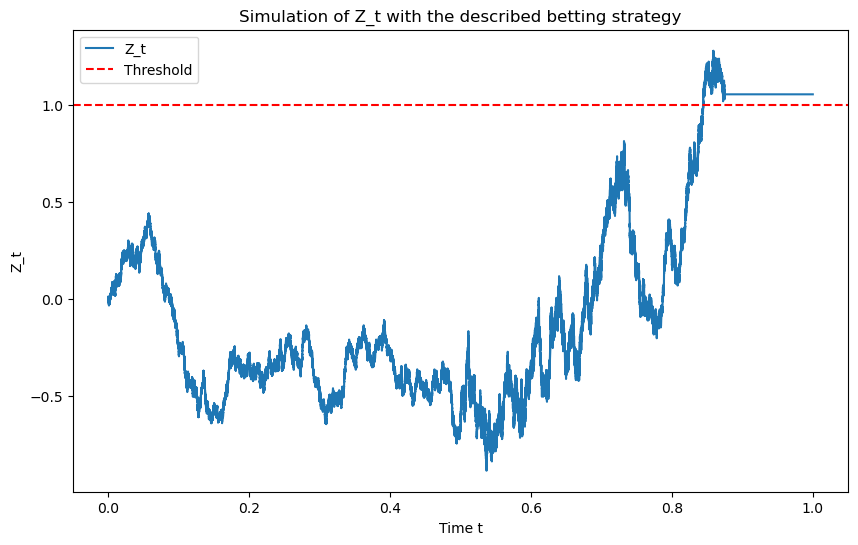
\includegraphics[width=0.76\linewidth]{REU-2024//Images/Betting Game.png}
    \caption{Martingale Betting Strategy}
    \label{fig:enter-label}
\end{figure}

\defn{Local Martingale}{A continuous process $M_t$ is adapted to the filtration $\{\calF_t\}$ is called a \textit{local martingale} on $[0,T)$ if there exists an icnreasing sequence of stopping times 
\[\tau_1\leq \tau_2 \leq \cdots\] such that with probability one,
\[\lim_{j\to \infty}\tau_j = T,\] and for each $j,$ 
\[M_t^{(j)} = M_{t\wedge {\tau_j}},\] is a martingale}
\rmkb{In the case of the stochastic integral, we let $\{\tau_j\}$ be the stopping times defined by 
\[\tau_j = \inf\{t: \langle Z \rangle_t = \int_0^t A_s^2 ds = j\}.\] Thus, for each $j,$ $M_t^{(j)}$ is a square integrate martingale, and so $Z_t$ is a local martingale on $[0,T),$ where 
\[T = \inf\{t: \int_0^t A_s^2 = \infty\}\]}
\rmkb{Suppose that \[dX_t = R_t dt + A_t dB_t,\] if $R_t \neq 0,$ then $X_t$ is not a martingale, and thus for $X_t$ to be a martingale, we need $R_t \equiv 0.$ It is a local martingale if $R_t \equiv 0$ but $X_t$ is not a martingale. We usually refer to $A_t dB_t$ as the local martingale part. }

\thm{Optional Sampling Theorem}{Suppose $Z_t$ is a continuous martingale and $T$ is a stopping time, both with respect to the filtration $\{\calF_t\}.$
\begin{itemize}
    \item If $M_t = Z_{t\wedge T},$ then $M_t$ is a continuous martingale with respect to $\{\calF_t\}$ and $\bbE[Z_{t\wedge T}] = \bbE[Z_0].$
    \item Suppose there exists $C< \infty$ such that for all $t,$ we have that $\bbE[Z_{t\wedge T}^2]\leq C.$ Then if $\bbP\{T< \infty\} = 1,$ $\bbE[Z_t] = \bbE[Z_0]$
\end{itemize}
}
\ex{Suppose $Z_t$ is a continuous martingale with $Z_0 = 0.$ Suppose that $a,b >0$ and let $T = \inf\{t | Z_t = -a \:\:or \:\:Z_t = b\}$. Suppose that $\bbP\{T< \infty\} = 1,$ (which happens if $Z_t$ is a standard Brownian motion. Then $Z_{t \wedge T}$ is  abounded martingale and thus 
\[0 = \bbE[Z_0] = \bbE[Z_t] = -a\bbP\{Z_T = a\} + b\bbP\{Z_t = b\},\] and thus
\[\bbP\{Z_t = b\} = \frac{a}{a+b}.\])}
\rmkb{The Martingale Convergence Theorem and the Maximal inequality also hold. }

\section{The Bessel Process}
The Bessel process with parameter $a$ is the solution to the SDE
\[dX_t = \frac{a}{X_t}dt + dB_t, \qquad X_0 = x_0>0.\]
Let $T_\epsilon = \inf\{t: X_t \leq \epsilon\},$ and note that there is no problem to find a solution for $t< T_\epsilon,$ and thus it is well defined for $t<T,$ where $T = T_0 = \inf\{t | X_t = 0\}.$ Thus, there is a strong drift close to $0.$ \newline 
Suppose that $0<r <R < \infty,$ and let 
\[\tau = \tau(r,R) = \inf\{t | X_t = r \: \: or \:\: X_t = R\}.\]
For $r\leq x \leq R,$ let 
\[\phi(x) = \bbP\{X_\tau = R | X_0 = x\},\]
and we'll use Ito's formula to compute $\phi.$
Note that $\phi(r) = 0, \phi(R) = 1.$ Let $J$ denote the indicator function of the event $\{X_\tau = R\}$
and let $M_t = \bbE[J  | \calF_t],$ we can use the tower property to show that $M_t$ is a martingale, and by the Markovian nature of the diffusion of $X,$
\[\bbE[J | \calF_t] = \phi(X_{t\wedge \tau})\] Thus, if $\tau \leq t,$ then we already know if $\{X_\tau = R\},$ but if $\tau >t,$ then the only useful information for predicting if $X_\tau = R$ is $X_t$ (Markov Property!). Thus, $\phi(X_{t \wedge \tau})$ must be a martingale. Ito's formula gives:
\[d\phi(X_t) = \phi'(X_t)dX_t + \frac{1}{2}\phi''(X_t)d\langle X\rangle_t = \left[\frac{a\phi'(X_t)}{X_t} + \frac{\phi''(X_t)}{2}\right]dt + \phi'(X_t)dB_t\]
But as seen before, if it is a martingale, then the $dt$ term must vanish. Thus, we must choose $\phi$ by solving the ODE
\[x\phi''(x) + 2a\phi'(x) = 0.\]
The solutions are of the form
\[\phi(x) = c_1 + c_2 x^{1-2a}, \qquad a\neq \frac{1}{2}\]
\[\phi(x) = c_1 + c_2 \ln(x), \qquad a= \frac{1}{2}\]
The boundary conditions, $\phi(r) = 0, \phi(R) = 1,$ determine that 
\begin{align}
    \phi(x) &= \frac{x^{1-2a} - r^{1-2a}}{R^{1-2a} - r^{1-2a}}, \quad a\neq \frac{1}{2}\\
    \phi(x) &= \frac{\ln(x) - \ln(r)}{\ln(R) - \ln(r)}, \quad a = \frac{1}{2}
\end{align}

\prop{If $a\geq \frac{1}{2},$ then $\bbP\{T  = \infty\} = 1,$ that is, with probability one, the Bessel process never reaches zero. If $a< \frac{1}{2},$ then $\bbP\{T< \infty\}=1.$}
\pf{Assume $X_0 = x <R$ and let $\tau(r,R)$ be defined as above. If $T< \infty,$ then there must be some $R<\infty$ such that $X_{\tau(r,R)} = r$ for all $r>0.$ Using the above equations, we see that 
\[\lim_{r\to 0}\bbP\{X_{\tau(r,R)} = r\} = \begin{cases}
    0, \qquad a\geq \frac{1}{2}\\
    1- (\frac{x}{R})^{1-2a}, \qquad a< \frac{1}{2}
\end{cases}\]}

\subsection{Feynman-Kac Formula}
Suppose that the price of a stock follows a geometric Brownian motion
\begin{align}
    dX_t = mX_tdt + \sigma X_t dB_t
\end{align}
Suppose further that at some future time $T$ we have an option to buy a share of the stock at price $S,$ but we'll only exercise the option if $X_t \geq S$ and the value of the option at time $T$ is $F(X_T),$ where
\[F(x) = (x-S)_+ = \max\{x-S, 0\}\]
This makes sense, because if $X_T\leq S,$ then $F(X_T) = 0,$ and thus there is no payoff, otherwise, you can buy the stock and sell it immediately on the market to make stonks.\newline\newline
Furthermore, suppose that there is an inflation rate of $r$ so that $x$ dollars at time $t$ in future is worth only $e^{-rt}x$ in current dollars. Let $\phi(t,x)$ be the expected value of this optino at time $t,$ measured in dollars at time $t,$ given that the current price of the stock is $x,$
\[\phi(t,x) = \bbE[e^{-r(T-t)}F(X_T) | X_t = x]\]
The Feynman-Kac formula gives a PDE for this quantity.
\newline\newline
Let's step it up, as it doesn't make a difference, and make the process a diffusion: Assume that $X_t$ satisfies the SDE
\[dX_t = m(t,X_t)dt + \sigma(t,X_t)dB_t, \quad X_0 = x_0\] and there is a payoff $F(X_T)$ at some future time $T.$ Suppose that there is an inflation rate $r(t,x)$ so that if $R_t$ denotes the value at time $t$ of $R_0$ dollars at time $0,$ then 
\[dR_t = r(t,X_t)R_tdt\]
\[R_t = R_0 \exp\{\int_0^t r(s,X_s)ds\}\] If $\phi(t,x)$ denotes the expected value of the payoff in time $t$ dollars given $X_t = x,$ then 
\[\phi(t,x) = \bbE\left[\exp\{-\int_t^T r(s,X_s)ds\} F(X_T) | X_t =x\right]\]
Using Ito's formula to derive a PDE for $\phi$ (assuming sufficient smoothness in $t$ and $x$), let 
\[M_t = \bbE[R_T^{-1}F(X_T) | \calF_t].\]
One can use the tower property to show that $M_t$ is a martingale, and since $R_t$ is $\calF_t-$measurable, 
\[M_t = R_t^{-1} \bbE[\exp\{\int_t^T r(s,X_s)ds\} F(X_T) | \calF_t]\]
But since $X_t$ ia markov process, it only cares about the information given by $X_t,$ and thus, by definition,
\begin{align}
    M_t = R_{t}^{-1}\phi(t,X_t)
\end{align}
and thus $M_t$ is a martingale. Ito's formula gives that
\[d\phi(t,X_t) = \partial_t \phi(t,X_t)  + \partial_x\phi(t,X_t)dX_t + \frac{1}{2}\partial_{xx}\phi(t,X_t)d\langle X\rangle_t.\]

In particular, 
\[d\phi(t,X_t) = H_tdt + A_tdB_t\]
with 
\[H_t = \partial_t \phi(t,X_t) + m(t,X_t)\partial_x \phi(t,X_t) + \frac{1}{2}\sigma(t,X_t)^2 \partial_{xx}\phi(t,X_t)\]
\[A_t = \sigma(t,X_t)\partial_x\phi(t,X_t).\] Since $\langle R\rangle_t = 0,$ the stochastic product rule implies that 
\[d[R_t^{-1}\phi(t,X_t)] = R_t^{-1}d\phi(t,X_t) + \phi(t,X_t)d[R_t^{-1}],\] and thus the $dt$ term is $R_t^{-1}$ times 
\[-r(t,X_t)\phi(t,X_t) + \partial_t\phi(t,X_t) + m(t,X_t) \partial_x\phi(t,X_t) + \frac{1}{2}\sigma(t,X_t)^2 \partial_{xx}\phi(t,X_t)\]
However, since $M_t$ is a martingale, this only happens if the $dt$ term is $0,$ and thus 
\[-r(t,X_t)\phi(t,X_t) + \partial_t\phi(t,X_t) + m(t,X_t) \partial_x\phi(t,X_t) + \frac{1}{2}\sigma(t,X_t)^2 \partial_{xx}\phi(t,X_t) = 0\]

\thm{Feynman-Kac Formula}{Suppose $X_t$ satisfies 
\[dX_t = m(t,X_t)dt +\sigma(t,X_t)dB_t, \quad X_0 = x_0\]
and $r(t,x)\geq 0$ is a discounting rate, and suppose that the payoff $F$ at time $T$ is given with $\bbE[|F(X_T)|]<\infty.$ If $\phi(t,x),0 \leq t \leq T$ is defined as 
\[\phi(t,x) = \bbE\left[\exp\{-\int_t^T r(s,X_s)ds\} F(X_T) | X_t =x\right]\] and $\phi(t,x)$ is $C^1$ in $t$ and $C^2$ in $x,$ then $\phi(t,x)$ satisfies the PDE
\[\partial_t\phi(t,x) = -m(t,x)\partial_x\phi(t,x) - \frac{1}{2}\sigma(t,x)^2\partial_{xx}\phi(t,x) + r(t,x)\phi(t,x)\] with $0\leq t < T,$ with terminal condition $\phi(T,x) = F(x).$
}

\ex{Suppose $X_t$ satisfies 
\[dX_t = mX_t dt + \sigma X_t dB_t,\] and $m(t,x) = mx, \sigma(t,x) = \sigma x,$ and $\phi$ is defined the same as above. Thus, the Feynman-Kac formula gives
\begin{align}
    \partial_t\phi = r\phi - mx\partial_x\phi - \frac{\sigma^2x^2}{2}\partial_{xx}\phi
\end{align} which is a version of the \textit{Black-Scholes PDE.}
}
\rmkb{Another derivation is given using the generator. Suppose that $X_t$ satisfies
\[dX_t = m(t,X_t)dt + \sigma(t,X_t)dB_t\] and that $F$ is a function which doesn't grow too quickly. Let 
\[f(t,x) = \bbE[F(X_T) | X_T = x].\]
Let $r(t)\geq 0$ be a discount rate and 
\[R_t = R_0 \exp\{\int_0^t r(s)ds\}\]
}

\chapter{Change of Measure and Girasanov Theorem}
\section{Absolutely Continuous Measures}
\defn{Absolutely and Mutually Continuous}{Supposse $\mu, \nu$ are measures on $(\Omega,\calF)$, then we say that 
\begin{itemize}
    \item $\mu$ is \textit{absolutely continuous} with respect to $\mu,$ written $\nu \ll \mu$ if for every $E \in \calF,$ if $\mu(E) = 0,$ then $\nu(E) = 0.$
    \item $\mu$ and $\nu$ are \textit{mutually absolutely continuous} or \textit{equivalent} measures if $\nu \ll \mu$ and $\mu \ll \nu.$
    \item $\mu$ and $\nu$ are \textit{singular} measures, written $\mu \perp \nu$ if there exists an event $E \in \calF$ with $\mu(E = 0$ and $\nu(\Omega\sm E) = 0$
\end{itemize}
}

\ex{
Let $\Omega$ be a countable set and $\calF = 2^\Omega,$ if $p:\Omega \to [0,\infty)$ is a function, then there exists a corresponding measure $\mu$ defined by 
\[\mu(E) = \sum_{\omega \in E}p(\omega)\]
Suppose $\nu$ is another measure given by the function $q,$ then let 
\[A_\mu = \{\omega : p(\omega) >0\}, \qquad A_\nu = \{\omega : q(\omega) >0\}\]

Then $\nu \ll \mu$ if and only if $A_\nu \subset A_\mu$ and 
\[q(\omega) = \frac{d\nu}{d\mu}(\omega)p(w)\]
where we define $d\nu/d\mu$ on $A_\mu$ by
\[\frac{d\nu}{d\mu}(\omega) = \frac{q(w)}{p(w)}\]
Thus, $\mu$ and $\nu$ are equivalent if $A_\nu = A_\mu$ and $\nu \perp \mu$ if $A_\nu \cap A_\mu = \emptyset.$

}

\thm{Radon-Nikodym Theorem}{Suppose $\mu$ and $\nu$ are $\sigma-$finite measures on $(\Omega, \calF)$ with $\nu \ll \mu,$ that is, 
\[\Omega = \bigcup_{n=1}^\infty A_n,\] with $\mu(A_n), \nu(A_n) < \infty$ for each $n.$ Then there exists a function $f$ such that for every $E,$ 
\[\nu(E) = \int_E fd\mu\]
}
\rmkb{The function $f$ is called the \textit{Radon-Nikodym derivative} of $\nu$ with respect to $\mu$ and is denoted 
\[f = \frac{d\nu}{d\mu}.\]}

\ex{
If $(\Omega, \calF, P)$ is a probability space, and $Q$ is a probability measure with $Q\ll P,$ then the Radon-Nikodym derivatve 
\[X = \frac{dQ}{dP}\] is a nonnegative random variable with $\bbE[X] = 1$ satisfying 
\[Q(E) = \bbE_P[X1_E]\] and extending it, 
\[\bbE_Q[Y] = \bbE_P[Y\frac{dQ}{dP}]\]

}

\ex{
Suppose $(\Omega, \calF, \bbP)$ is a probabilty space and $\calG \subset \calF.$ Let $X$ be a nonnegative integrable $\calF-$measurable random variable. Then 
\[Q(A) = \bbE[X 1_A], \quad A \in \calG\] defined a measure on $(\Omega, \calG)$ that satisfied $Q\ll \bbP.$ This, there exists a $\calG-$measurable random variable $Y$ such that for all $A \in \calG,$ 
\[Q(A) = \bbE[1_A Y],\] we can say that $Y$ is the conditional expectation $E(X | \calG).$

}

\subsection{Giving Drift to a Brownian Motion}
To take a fair game and make it unfair (or vice-versa):
\begin{itemize}
    \item Add a deterministic amount in one direction.
    \item Change the probabilities of the outcome. 
\end{itemize}

For the first method, define a Brownian motion with drift $m$ by setting
\[W_t = mt + B_t\]

For the second way, suppose $B_t$ is defined on the probability space $(\Omega, \calF, \bbP)$ with a filtration $\{\calF_t\}.$ To change the probability, we must consider a measure $Q$ instead of $\bbP,$ and so let 
\[M_t = e^{mB_t - \frac{m^2 t}{2}}.\] It can be derived that $M_t$ is a martingale, and that $M_t$ satisfies 
\[dM_t = mM_tdB_t, M_0 = 1\] If $V$ is $\calF_t$ measurable, then define 
\[Q_t(V) = \bbE[1_V M_t]\] and thus 
\[\frac{dQ_t}{d\bbP} = M_t\]
it is easy to see that if $s<t$ and $V$ is $\calF_s-$measurable, then it is also $\calF_t-$Measurable, that is, $Q_s(V) = Q_t(V):$
\begin{align*}
    Q_s(V) &= \bbE[1_V M_t]\\
    &= \bbE[\bbE[1_V M_t | \calF_s]]\\
    &= \bbE[1_V M_s]\\
    &= Q_s(V)
\end{align*}
Moreover, we claim that the process $t\to B_t$ under the measure $Q$ is a Brownian motion with drift $m$ and $\sigma^2 = 1.$



\ex{Suppose $X_t$ is a geometric Brownian motion satisfying 
\[dX_t = X_t[m dt + \sigma dB_t],\] where $B_t$ is a standard Brownian motion defined on the probability space $(\Omega, \calF, \bbP.)$ If $r\in \bbR,$ then we can find a new probability measure $Q$ such that $dB_t = rdt + dW_t,$ where $W_t$ is a Brownian motion with respect to $Q.$ Then 
\[dX_t = X_t[(m + \sigma r)dt + \sigma dW_t]\] Thus, with respect to $Q,$ $X_t$ is a geometric Brownian motion with the same volatility but new drift. Thus, measures for GBM with the same $\sigma$ are equivalent. }

\section{Girsanov Theorem}

Suppose $M_t$ is a nonnegative martingale satisfying the exponential SDE
\begin{align}
    dM_t = A_tM_t dB_t, \quad M_0 = 1,
\end{align}
where $B_t$ is SBM. The solution to this equation, derived before, is
\begin{align}
   M_t = e^{Y_t}, \qquad Y_t = \int_0^t A_sdB_s - \frac{1}{2}\int_0^t A_s^2 ds 
\end{align}
Assume $M_t$ is a martingale, and thus we can define a probability measure $\bbP^*$ such that is $V$ is a $\calF+_t$ measurable event, then 
\begin{align}
    \bbP^*(V) = \bbE[1_V M_t.]
\end{align}Thus, 
\[\frac{d\bbP^*}{d\bbP} = M_t\] If $s<t $ and $V$ is $\calF_s$ measurable, then $V$ is also $\calF_t-$measurable, and thus we need that for such $V,$
\[\bbE[1_V M_s] = \bbE[1_V M_t]\]
Let $\bbE^*$ denote expectations with respect to $\bbP^*.$ If $X$ is $\calF_t-$measurable, then 
\[\bbE^*[X] = \bbE[XM_t]\]

\thm{Girsanov Theorem}{Suppose $M_t$ is a nonnegative martingale satisfying (10.1) and let $\bbP^*$ be the probability measure define in (10.3). If 
\[W_t = B_t - \int_0^t A_s ds,\] then with respect to the measure $\bbP^*,$ $W_t$ is a standard Brownian motion. Thus
\[dB_t = A_tdt + dW_t,\] where $W$ is a $\bbP^*-$Brownian motion.}
\rmk{If we weight the probability measure $\bbP$ by the martingale, then in the new measure $\bbP^*,$ the Brownian motion acquires a drift $A_t.$}

To prove this, consider two lemmas:
\lem{Lemma A}{Let $0\leq t \leq T$ and let $Y$ be a $\calF_t$ measurable random variable, then 
\[\bbE^*[Y] = \bbE[YZ(t)]\]}
The proof is definitions.
\lem{Lemma B}{Let $s\leq t$ such that $0\leq s \leq t\leq T$ and $Y$ be an $\calF(t)-$measurable random variable, then 
\[\bbE^*[Y | \calF(s)] = \frac{1}{Z(s)}E[YZ(t) | \calF(s)], \qquad a.s\]}

\pf{
Note that by definition, the RHS is $\calF_s$ measurable. 
\begin{align*}
    \int_A \frac{1}{Z(s)} E[YZ(t) | \calF_s]d\bbP^* &= \int_\Omega 1_A\frac{1}{Z(s)} E[YZ(t) | \calF_s]d\bbP^*\\
    &= \bbE^*[1_A\frac{1}{Z(s)} E[YZ(t) | \calF_s]]\\
    &= \bbE[1_AE[YZ(t) | \calF_s]]\\
    &= \bbE[E[1_AYZ(t) | \calF_s]]\\
    &= \bbE[1_A YZ(t)]\\
    &= \bbE^*[1_A Y]\\
    &= \int_AY d\bbP^*
\end{align*}
where the second to last equality follows from Lemma A.

\begin{align*}
    \int_A \bbE^*[Y | \calF_s] d\bbP^* &= \int_A Y d\bbP^* 
\end{align*}
for all $A \in \calF_s$
}
\pf{By definition, $W(0) = 0,$ and is continuous. We know that 
\[dW_t = dW_t  + A_t dt\] and thus, by a formal derivation, 
\[\langle W\rangle_t = t\] We have showed via Ito's formula already that $M_t$ is a martingale and $\bbE[M_t] =1.$
Because 
\[M_t = \bbE[M_t | \calF_t] = \bbE[M | \calF_t],\] then $M_t$ is a Radon-Nikodyn process. We claim that $\{W_t M_t\}$ is martingale:
\begin{align*}
    d(W_tM_t) &= W_tdM_t + M_tdW_t + dW_tdM_t, \quad \text{(Ito's Product rule)}
    &= -W_tA_tM_tdW_t + Z_t(dW_t - A_tdt)\\
    &= (-W_t-A_t +1)M_tdW_t
\end{align*}
and thus $W_tM_t$ is an Ito integral, and thus a martingale.\newline
Thus, by Lemma B, if $s<t$:
\begin{align}
    \bbE^*[W_t | \calF_s] &= \frac{1}{M_s}\bbE[W_tM_t | \calF_s]\\
    &= \frac{1}{Z(s)}W_s M_s\\
    &= W_s
\end{align}
and thus $W_t$ is a martingale, and by Levy's theorem, $W_t$ is a Brownian motion. 
}


\thm{Girsanov Theorem, local martingale form}{Suppose $M_t = e^{Y_t}$ satisfies (10.1) - (10.2), and let 
\[T_n = \inf\{t | M_t  + |A_t| = n\}, \qquad T = T_{\infty} = \lim\limits_{n\to \infty}T_n.\] Let $\bbP^*$ be the probability measure as above. If 
\[W_t = B_t - \int_0^tA_s ds, \quad 0\leq t <T,\] then with respect to the measure $\bbP^*,$ $W_t,$ $t<T,$ is a standard Brownian motion. In other words, 
\[dB_t = A_tdt + dW_t, \qquad t<T,\] where $W$ is a $\bbP^*-$Brownian motion. If any of the three following conditions holds, then $M_s,$ $0\leq s\leq t,$ is actually a martingale:
\[\bbP^*\{T>t\} =1\]
\[\bbE[M_t] =1\]
\[\bbE[\exp\{\frac{\langle T\rangle_t}{2}\}]< \infty/\]
}

\rmkb{The last condition is called the novikov condition}

\section{The Black-Scholes Formula}
\defn{Arbitrage}{An \textit{arbitrage} is a system that guarantees that a player  will not lose money while also giving  a positive probability of making money.}
\rmkb{
 If $P$ and $Q$ are equivalent probability measures, then an arbitrage under probability $P$ is the same as an arbitrage under probability $Q,$ because for probability measures:
 \[P(V) = 0 \Leftrightarrow Q(V) = 0\]
 \[P(V)>0 \Leftrightarrow Q(V) >0\]
}
Consider a simple European call option for a stock whose price moves according to a geometric Brownian motion:
\[dS_t = S_t[mdt + \sigma dB_t]\] and there exists a risk-free bound $R_t$ such that
\[dR_t = rR_t dt\]
That is, $R_t = e^{rt}R_0.$\newline\newline Let $T$ be a time in the future and suppose we have the option to buy a share of stock at time $T$ for strike price $K.$ The value of this option at time $T$ is:
\[F(S_T) = (S_T - K)_+ = \begin{cases}
    (S_T - K), \quad \text{if} S_T >K,\\
    0, \quad \text{if} S_T \leq K.
\end{cases}\]
The goal is to find the price $f(t,x)$ of the option at time $t<T$ given $S_t = x$
One option, using the Feynman-Kac formula, is to price the option using
\[f(t,x) = \bbE[e^{-r(T - t)F(S_T) | S_t =x}],\] which satisfies the PDE:
\[\partial_t f(t,x) = rf(t,x) - mx\partial_x f(t,x) - \frac{\sigma^2 x^2}{2}\partial_{xx}f(t,x)\]

The Black-Scholes approach is to let $f(t,x)$ be the value of a portfolio at time $t,$ given that $S_t = x,$ that can be hedged in order to guarantee a portfolio of value $F(S_T)$ at time $T.$ Where a portfolio is an ordered pair $(a_t, b_t),$ where $a_t, b_t$ denote the number of units of stocks and bonds, respectively. Let $V_t$ be the value of the portfolio at time $t,$
\begin{align}
    V_t = a_tS_t + b_tR_t
\end{align}

We will manage the portfolio by switching between stocks and bonds, so that no matter how the price of the stock moves, the value at time $T$ will be 
\[V_T = (S_T - K)_+\]
Assume that the portfolio is \textit{self financing}, that one does not add outside resources to the portfolio, and thus the change of value of the portfolio is given by the change of the price of the assets,
\begin{align}
   dV_t = a_tdS_t + b_tdR_t 
\end{align}
This is not a direct consequence of 10.7, since $a_t,b_t$ vary with time and are not constant, we need to utilize the product rule:
\[d(a_tS_t)= da_t + a_tdS_t + d\langle a,S\rangle_t\]
\[d(b_tR_t) = b_tdR_t + R_tdb_t\]
Thus we can see that 10.8 is a strong assumption about the portfolio. Thus, assuming 10.7 and plugging in:
\begin{align}
    dV_t &= a_tS_t[mdt + \sigma dB_t] + b_r rR_t dt \nonumber\\
    &= a_tS_t[mdt + \sigma dB_t]  + r[V_t - a_tS_t]dt\nonumber\\
    &= [ma_t S_t + r(V_t - a_t S_t)]dt + \sigma a_tS_t dB_t
\end{align}
By definition, $V_t = f(t,S_t),$ and thus assuming sufficient smoothness, Ito's formula shows that 
\begin{align}
    dB_t &= df(t,S_t)\nonumber\\
    &= \partial_t f(t,S_t)dt + \partial_x f(t,S_t)dS_t + \frac{1}{2}\partial_{xx}f(t,S_t)d\langle S \rangle_t\nonumber\\
    &= \left[\partial_t f(t,S_t) + mS_t\partial_x f(t,S_t) + \frac{\sigma^2 S_t^2}{2}\partial_{xx}f(t,S_t)\right]dt \sigma S_t \partial_x f(t,S_t)dB_t
\end{align}
By equating $dB_t$ terms in the two above equation, we can see that the portfolio is given by
\begin{align}
    a_t &= \partial_x f(t,S_t)\qquad b_t = \frac{V_t - a_tS_t}{R_t}
\end{align}
By equating the $dt$ terms we get the Black-Scholes equation
\[d_t f(t,x) = rf(t,x) - rx\partial_x f(t,x) - \frac{\sigma^2 x^2}{2}\partial_{xx}f(t,x)\]
\begin{itemize}
    \item $m,$ the drift term does not appear, and is the same as Feynman-kac but with $m$ replaced with $r,$  and thus we can write
    \[f(t,x) = \bbE[e^{-r(T-t)F(S_t)} | S_t = x]\] where $S$ satisfies 
    \[dS_t = S_t[rdt + \sigma dB_t]\]
\end{itemize}
We can use this and compute the Black-Scholes formula:
\begin{align}
    f(T-t,x) = x\Phi \left(\frac{\log(x/K) + (r + \frac{\sigma^2    }{2})t}{\sigma\sqrt{t}}\right) - Ke^{-rt}\Phi\left(\frac{\log(x/K) + (r-\frac{\sigma^2}{2})t}{\sigma\sqrt{t}}\right)
\end{align}

We can generalize this to the case when the stock price satisfies 
\[dS_t = S_t [m(t,S_t)dt + \sigma(t,S_t)dB_t]\]
\[dR_t = r(t,S_t)R_tdt\]
We again get (10.9) and (10.10) and by equating coefficients we get the Black-Scholes equation
\begin{align}
    \partial_t f(t,x) = r(t,x)f(t,x) - r(t,x)x\partial_xf(t,x) - \frac{\sigma(t,x)^2 x^2}{2}\partial_{xx}f(t,x)
\end{align}
The function $f$ can be given by 
\[f(t,x) = \bbE[R_t/R_T]F(S_T) | S_t = x\]
given that $S_t,R_t,$ satisfy
\[dS_t = S_t[r(t,S_t)dt + \sigma(t,S_t)dB_t]\]
\[dR_t = r(t,S_t)R_t dt\]

\section{Martingale approach to Black-Scholes equation}
Suppose the risk-free bond has rate $r(t,x)$ and the volatility is given by $\sigma(t,x).$ If $R_t$ denotes the value of the bond at time $t,$ then 
\[dR_t = r(t,S_t)R_tdt, \qquad R_t = R_0\exp\{\int_0^t r(s,S_s)ds\},\] we must also assume that the stock satisfies
\begin{align}
    dS_t = S_t[r(t,S_t)dt + \sigma(t,S_t)dB_t]
\end{align}
and the value of the portfolio at time $t$ satisfies
\[V_t = f(t,S_t) = \bbE_Q[(R_t/R_T)F(S_T) | S_t] = \bbE_Q[(R_t/R_T)F(S_T) | \calF_t].\] where $\bbE_Q$ is the expectation taken with respect to the probability measure which $S_t$ satisfies (10.14). \newline\newline
Let $\Tilde{S}_t = \frac{S_t}{R_t},$ $\Tilde{V}_t = \frac{V_t}{R_t}$ be the stock price and the porfolio bounded discounted by the bond rate. The product rule shows that $\Tilde{S}_t$ satisfies
\[d\Tilde{S}_t = \sigma \Tilde{S}_t dB_t\] and thus $\Tilde{S}_t$ is a martingale, and 
\[\Tilde{V}_t = \frac{V_t}{R_t} = \frac{\bbE_Q[(R_t/R_T)F(S_T) | \calF_t]}{R_t} = \bbE_Q[\frac{F(S_T)}{R_T} | \calF_t] = \bbE_Q[\Tilde{V}_T | \calF_t]\]

\thm{What we derived above}{Suppose $S_t$ satisfies \[dS_t = S_t[m(t,S_t)dt + \sigma(t,S_t)dB_t]\] and a risk-free bond $R_t$ is available at rate $r(t,S_t),$
\[dR_t = r(t,S_t)R_t dt\] Suppose that the Brownian motion is defined on a probability space $(\Omega, \calF, \bbP)$ and that there exists a probability measure $Q$ that is an equivalent measure to $\bbP$ such that under $\bbQ,$ the discounted stock price $\Tilde{S}_t = \frac{S_t}{R_t}$ is  a martingale. Suppose there is an option at time $T$ with value $F(S_T)$ such that $\bbE[\frac{|F(S_T)|}{R_T}]<\infty,$ then the arbitrage-free price of the option at time $t$ is 
\[V_t = R_t \bbE_Q(\frac{f(S_T)}{R_T} | \calF_t)\]
}

\ex{
Ok. This is fucking it. Let's derive this shit.\newline\newline
Suppose $r, \sigma$ are constants and $F(S_T) = (S_T - K)_+.$ The discounted values are $\Tilde{S}_t = e^{-rt}S_t,$ and $\Tilde{V}_t = e^{-rt}V_t,$ and 
\[\Tilde{V}_T = e^{-rT}F(S_T) = e^{-rT}(S_T - K)_+ = (\Tilde{S}_T - \Tilde{K})_+\] where $\Tilde{K} = e^{-rt}K.$ nder the measure $Q,$ $\Tilde{S}_t$ satisfies 
\[d\Tilde{S}_t = \sigma \Tilde{S}_t dB_t\] implying that 
\begin{align*}
    \Tilde{S}_T &= \Tilde{S}_t \exp\left\{\int_t^T \sigma dB_s - \frac{1}{2}\int_t^T \sigma^2 ds\right\}\\
    &= \Tilde{S}_t \exp\left\{\sigma(B_T - B_t) - \frac{\sigma^2(T - t)}{2}\right\}
\end{align*}
Thus, the conditional distribution of $\Tilde{S}_T$ given $\Tilde{S}_t$ is that of 
\[Z = \exp\{aN + y\}\] given that $a = \sigma\sqrt{T - t},$ $N$ is standard normal, and 
\[y = \log \Tilde{S}_t - \frac{a^2}{2}\]
It takes little work to show that $Z$ has density
\[g(z) = \frac{1}{az}\phi(\frac{-y + \log(z)}{a})\] where $\phi$ is the standard normal density, and thus, 
\[\Tilde{V}_t = \int_K^\infty (z-\Tilde{K})g(z) dz\]
More calculus gives
\[\Tilde{V}_t = \Tilde{S}_t \Phi\left(\frac{\log(\Tilde{S}_t/\Tilde{K}) + \frac{a^2}{2}}{a}\right) - \Tilde{K}\Phi\left(\frac{\log(\Tilde{S}_t/\Tilde{K} - \frac{a^2}{2})}{a}\right)\]
Implying that 
\[V_t = e^{rt}\Tilde{V}_t = {S}_t \Phi\left(\frac{\log(S_t/{K}) + rs  + \frac{a^2}{2}}{a}\right) - e^{-rs}{K}\Phi\left(\frac{\log({S}_t/{K}  + rs - \frac{a^2}{2})}{a}\right)\]}

where $s = T-t,$ and thus plugging in $a = \sigma\sqrt{s}$ gives the Black Scholes Formula!\newpage
One of the hypothesis in the above Theorem is that if $S_t$ satisfies 
\[dS_t = S_t[m(t,S_t)dt + \sigma(t,S_t)dW_t],\]
then there exists a probability measure $Q$ under which 
\begin{align}
   dS_t = S_t[r(t,S_t)dt + \sigma(t,S_t)dW_t] 
\end{align}
Where $W_t$ is a $Q-$Brownian motion. Thus, if $S_t$ satisfies (10.15), then the discount price satisfies
\begin{align}
    d\Tilde{S}_t = \Tilde{S}_t \sigma(t,S_t)dW_t
\end{align}
The Girsanov theorem tells us that the way to obtain $Q$ is to tilt by the local martingale $M_t,$ where 
\[dM_t = M_t \frac{r(t,S_t) - m(t,S_t)}{\sigma(t,S_t)}dB_t\] and thus in the measure $Q,$
\[dB_t = \frac{r(t,S_t) - m(t,S_t)}{\sigma(t,S_t)}dt + dW_t \]

\section{Martingale approach to pricing}
\begin{figure}[h!]
    \centering
    
\includegraphics[width=0.5\linewidth]{REU-2024//Images/SDE.jpg}
    \caption{Agus Thrm}
    \label{fig:enter-label}
\end{figure}

Suppose $S_t$ denotes the price of an asset satisfying 
\[dS_t = S_t[m_t dt + \sigma_t dB_t]\]
where $B_t$ is a standard Brownian motion. Let $\calF$ denote the information in $\{B_s | 0\leq s \leq t\},$ and as usual assume that $m_t, \sigma_t$ are processes adapted to the filtration $\{\calF_t\}.$ Assume that there is a risk-free bond $R_t$ satisfying 
\[dR_t = r_tR_tdt, \qquad R_t = R_0 \exp\{\int_0^t r_s ds\}\]
where $r_t$ is adapted. Let $T$ be a fixed future time and assume that $V$ is an $\calF_t-$measurable random valuable. We say that $V$ is a claim at time $T,$ such as 
\[V = F(S_T), \quad V = \max\{0\leq t\leq T\}S_t, \quad V = \frac{1}{T}\int_0^T S_t dt\]
\defn{Arbitrage-free price}{If $V$ is a claim at time $T,$ then the \textit{(arbitrage-free) price} $V_t,$ $0\leq t\leq T,$ of a claim $V_T$ is the minimum value of a self-financing portfolio that can be hedged to guarantee that its value at time $T$ is $V.$}
\rmkb{The goal is to determine the price $V_t$ and the portfolio, $(a_t,b_t,)$ where $a_t$ denotes the number of units of $S_t$ and $b_t$ the number of units f $R.$}
Recall:
\[V_t = a_tS_t + b_tR_t\]
and $(a_t,b_t)$ is self-financing if
\[dV_t = a_tdS_t + b_tdR_t\]
Let 
\[\Tilde{S}_t = \frac{R_0}{R_t}S_t, \qquad \Tilde{V}_t = \frac{R_0}{R_t}V_t\]
denote the discount stock price and discount value, the latter of which is given by 
\[\Tilde{V}_t = a_t \Tilde{S}_t + b_tR_0\]
And thus, using the product formula, we get that 
\[d\Tilde{S}_t = \Tilde{S}_t[(m-r_t)dt + \sigma_tdB_t]\]
\rmkb{Our goal is to find a self-financing portfolio $(a_t,b_t)$ such that with probability one, 
\[\Tilde{V}_T = a_T\Tilde{S}_t + b_TR_0 = \Tilde{V}\]}
Let $Q$ be the probability measure that is an equivalent measure with respect to $\bbP$ such that $\Tilde{S}_t$ under $Q$ is a martingale. By Example 5.3.3 on Lawler, Girsanov tells us to choose
\[dQ = M_td\bbP\] where $M_t$ satisfies
\begin{align}
    dM_t = \frac{r_t - m_t}{\sigma_t}M_tdB_t, \quad M_0 = 1
\end{align}
\begin{itemize}
    \item Assumption 1: The local martingale defined in 10.17 is a martingale. Let 
    \[W_t = B_t - \int_0^t \frac{r_s - m_s}{\sigma_s}ds\] be the Brownian motion with respect to $Q.$ Plugging into the $d\Tilde{S}_t$ differential,
    \begin{align}
        d\Tilde{S}_t = \sigma \Tilde{S}_tdW_t
    \end{align}
    \item Assumption 2: The $Q-$local martingale $\Tilde{S}_t$ satisfying (10.18) is a $Q-$martingale
\end{itemize}

\defn{Contingent Claim}{A claim $V$ at time $T$ is called a \textit{contingent claim} if $V\geq 0$ and \[\bbE_Q[\Tilde{V}^2]<\infty\]}
\rmkb{
The \textit{(arbitrage-free) price} $V_t$ $0\leq t\leq T$ of a contingent claim $V_T$ is the minimum value of a self-financing portfolio that can be hedged to guarantee that its value never drops below zero and at time $T$ equals $V.$
}
Given a contingent claim, set 
\[\Tilde{V}_t = \bbE_Q[\Tilde{V} | \calF_t]\]
Thus, $\Tilde{V}_t$ is a square integrable martingale. Assume there exists a process $A_t$ such that
\begin{align}
d\Tilde{V}_t = A_t dW_t    
\end{align}
then:
\begin{align*}
    dV_t &= R_td\Tilde{V}_t + \Tilde{V}_tdR_t\\
    &= R_tA_tdW_t + \Tilde{V}_t dR_t\\
    &= \frac{A_t}{\sigma^t\Tilde{S}_t}R_td\Tilde{S}_t + \Tilde{V}_tdR_t\\
    &= \frac{A_t}{\sigma^t\Tilde{S}_t}[dS_t - \Tilde{S}_tdR_t] + \Tilde{V}_tdR_t\\
    &= \frac{A_t}{\sigma\Tilde{S}_t}dS_t + \left[\Tilde{V}_t - \frac{A_t}{\sigma_t}\right]dR_t
\end{align*}
Thus, if 
\begin{align}
    a_t = \frac{A_t}{\sigma_t\Tilde{S}_t}, \qquad b_t = \Tilde{V}_t - \frac{A_t}{\sigma_t}
\end{align}
then the portfolio is self financing and a simple calculation shows that 
\[a_tS_t + b_t R_t = V_t\]
\begin{itemize}
    \item Assumption 3: We can write $\Tilde{V}_t$ as (10.19) and if $a_t,b_t$ are defined as in (10.20), then 
    \[V_t = \int_0^ta_sdS_s + \int_0^tb_sdR_s\] is well defined.
\end{itemize}

\thm{Above stuff}{If $V$ is a contingent claim and assumptions 1-3 hold, then the arbitrage-free price is $V_t = R_t E_Q[\Tilde{V}_T | \calF_t]$}
\ex{
This is the end. Close your eyes and count to 10.\newline\newline
Assume that the stock price is a diffusion satisfying 
\[dS_t = S_t[m(t,S_t)dt + \sigma(t,S_t)dB_t]\]
and the bond rate satisfies
\[dR_t = r(t,S_t)R_tdt.\]
The product rule then implies that the discounted stock price satisfies
\[d\Tilde{S}_t = \Tilde{S}_t[(m(t,S_t) - r(t,S_t))dt + \sigma(t,S_t)dB_t]\]
Given some claim $V$ of the form $V = F(S_T),$ let $\phi$ be the function
\[\phi(t,x) = \bbE_Q[(R_t/R_T)V | S_T = x]\] and note that 
\[V_t = \phi(t,S_t)\]
}
Using Ito's formula and recalling that 
\[dS_t = S_t[r(t,S_t)dt + \sigma(t,S_t)dW_t,\] we see that 
\[d\Tilde{V}_t = d[R_t^{-1}\phi(t,S_t)] = J_tdt + A_tdW_t\] where 
\[J_t = R_{t}^{-1}[\partial_t\phi(t,S_t) + \frac{\sigma(t,S_t)^2S_t^2 }{2}\partial_{xx}\phi(t,S_t) + r(t,S_t) S_t\partial_x\phi(t,S_t) - r(t,S_t)\phi(t,S_t)]\]
\[A_t = R_t^{-1} S_t\sigma(t,S_t)\partial_x\phi(t,S_t) = \Tilde{S}_t\sigma(t,S_t)\partial_x\phi(t,S_t)\]
Since $\Tilde{V}_t$ is a $Q-$martingale, $J_t = 0,$ giving the Black-Scholes PDE. Since $d\Tilde{V}_t = A_tdW_t,$ then plugging into (10.20), we get 
\[a_t = \partial_x(t,S_t)\]
\[b_t = R_t^{-1}[V_t - S_t\partial_x(t,S_t)]\]










































































































































































































\end{document}
